%=========================================================================

\chapter{Úvod}
%=========================================================================
% Introduction for Marek Kidon's thesis

\externaldocument{obsah}

Tato pr�ce se zab�v� evolu�n�m n�vrhem ha�ovac�ch funkc�. Ha�ovac� 
funkce jsou ji� dob�e zavedenou a neodmyslitelnou sou��st� modern�ho
po��ta�ov�ho sv�ta. Jejich uplatn�n� je ��rok�, nicm�n� nej�ast�ji se s
nimi setk�v�me v kryptografii (kryptografick�mi ha�ovac�mi funkcemi se
v�ak v t�to pr�ci zab�vat nebudeme) a ha�ovac�ch tabulk�ch. Ha�ovac�
tabulky jsou v�znamn� a hojn� vyu��van� vyhled�vac� datov� struktury, 
kter� p�i vhodn�m zvolen� ha�ovac� funkce pracuje velmi rychle a 
efektivn�. Tradi�n� n�vrh vhodn� ha�ovac� funkce pro zadanou aplika�n� 
dom�nu nen� trivi�ln� �kol. Pomoci si v�ak m��eme i m�n� tradi�n�mi 
metodami n�vrhu. Jednou z nich je i n�vrh zalo�en� na evol�n�ch 
algoritmech neboli evolu�n� n�vrh. Inspirac� pro evolu�n� n�vrh je jev 
biologick� evoluce. Evolu�n� algoritmy obecn� pracuj� nad populac� 
kandid�tn�ch �e�en�, kde ka�d� kandid�tn� �e�en� je pr�v� jeden jedinec. 
Pro vytvo�en� nov� populace jedinc� se pou��vaj� 
biologi� inspirovan� oper�tory. My�lenka spo��v� v postupn�m prohled�v�n� 
prostoru mo�n�ch �e�en� dokud nenalezneme takov�, kter� sv�mi vlastnosti 
bude p�evy�ovat n�mi stanoven� pr�h, kde jeden krok itera�n�ho 
prohled�vac�ho algoritmu je pr�v� jedna generace.

V kapitole 2 se budeme bl��e zab�vat ha�ov�n�m. Neprve si zavedeme 
nezbytn� pojmy a v n�vaznosti si pop��eme, jak funguj� ha�ovac� tabulky a 
jak je d�le�it� vhodn� zvolit ha�ovac� funkci, pop��pad� jak� dopad na 
v�konnost ha�ovac� tabulky m� nevhodn� zvolen� ha�ovac� funkce.

Kapitola 3 bude zam��ena na evolu�n� n�vrh. Pop��eme si, jakou roli hraje evolu�n� n�vrh v kontextu po��t�n� podle p��rody (natural computing). Uvedeme a vysv�tl�me si pr�ci obecn�ho evolu�n�ho algoritmu a zm�n�me si jednotliv� odv�tv�, kter� spadaj� pod evolu�n� algoritmy. 

N�sleduj�c� kapitola 4 bude v�nov�na n�vrhu �e�en�. V �vodu t�to kapitoly 
si vysv�tl�me, pro� je vhodn� navrhovat ha�ovac� funkce evolu�n�. Uvedeme 
zvolenou metodu evolu�n�ho n�vrhu a pop��eme si jej� parametry. Sou��st� 
bude tak� popis fitness funkce, tedy to co budeme pova�ovat za d�le�it� a 
podle �eho se budeme rozhodovat p�i hled�n� na�eho po�adovan�ho �e�en�.
%=========================================================================


\chapter{Hašování}
\label{sec:hashing}
Hašovací tabulky jsou důležitou součástí moderního světa informačních 
technologíí. Jsou to vyhledávací datové struktury, které nám za určitých
okolností umožní vyhledávat, vkládat a mazat uložené položky s konstantní
časovou složitostí. Jedná se o jednu z několika možných implementací
asociativního pole. Ty další jsou například stromové implementace, 
implementace vázaným seznamem s lineáním průchodem a další. Žádnými
z těchto implementací se zde zabývat nebudeme \cite{art_of_programming}.

\section{Princip}
Mějme dané univerzum klíčů $U$, kde některé klíče $k \in U$ si přejeme
asociovat s nějakými satelitnímy daty $v$, jejichž povaha není pro nás v
tuto chvíli důležitá. Dále máme dynamickou množinu $S = \{(k,v) | k \in u\}$
uchovávající klíče s jejich satelitními daty. Pak nad množinou $S$ chceme
pro nějaký klíč $k$ a některé její položky $x=(k, v)$ provádět následující 
operace: 

\begin{enumerate}
	\item \textit{vkládání} dat, tedy operaci 
		$Insert(S,x) : S \to S \cup \{(k, v)\} $,

	\item \textit{mazání} dat, tedy operaci 
		$Delete(S,x) : S \to S - \{(k, v)\}$

	\item \textit{výhledávání} satelitních dat podle zadaného klíče,
		tedy operaci \newline $Search(S,k) : 
			\begin{cases}
				x 	: x.k = k \\
				nil : jinak 
			\end{cases} $
\end{enumerate}

Operace vyhledávání není totální, musíme tedy explicitně vhodně ošetřit
případy, kdy se prvek $x=(k,v)$ v tabulce nevyskytuje.

Nejjedodušší implementací je \textit{tabulka s přímým přístupem} za
předpokladů, že $|U|$ je přijatelná. Uvažme například univerzum
klíču $U = \{0,1,2,3,\ldots,m-1\}$, a tabulku $T$ reprezentující
dynamickou množinu $S$, pak nejjednodušším přístupem je použít jako
klíče přímo prvky množiny $U$. Pak operace vyhledávání je rovna operaci
přístupu do tabulky na zadanou lokaci, například $Search(T,k) = T[k]$
pro nějaký klíč $k \in U$.

Může však nastat případ, kdy $m$ bude příiš velké číslo. Typickým příkladem
jsou klíče množiny všech možných řetězců. Pak by tabulka s přímým přístupem
byla příliš velká a nevhodná pro moderní počítače. Pokud potřebujeme 
vyhledávat pouze v nějaké podmnožině $K \subset U$, kde $|K| << |U|$, je 
vhodné použít hašovací funkci. Zjevnou výhodou tabulek s přímým přistupem je složitost
, která je $\theta (1)$ v nejhorším případě. Nevýhodou je paměťová náročnost
pro velká univerza $U$, kdy velká část tabulky zůstane prázdná.

\subsection{Hašovací funkce}
Hašovací funkce je zobrazení, mapující prvky množiny $U$ na jednotlivé 
sloty (indexy) tabulky $T$ :
$$ f_{hash} : U \to (0,1,\ldots,m-1)$$
za předpokladu, že tabulka má právě $m-1$ slotů. Vyhledávací struktura 
složená z dynamické množiny $S$ reprezentovanou tabulkou $T$ a hašovací 
funkcí $f_{hash}$ se nazývá \textit{hašovací tabulka} 
viz. \ref{fig:hash_table_example}.

%%%%%%%%%%%%% HASH TABLE EXAMPLE %%%%%%%%%%%%%%%
\begin{figure}[!ht]
	\centering
	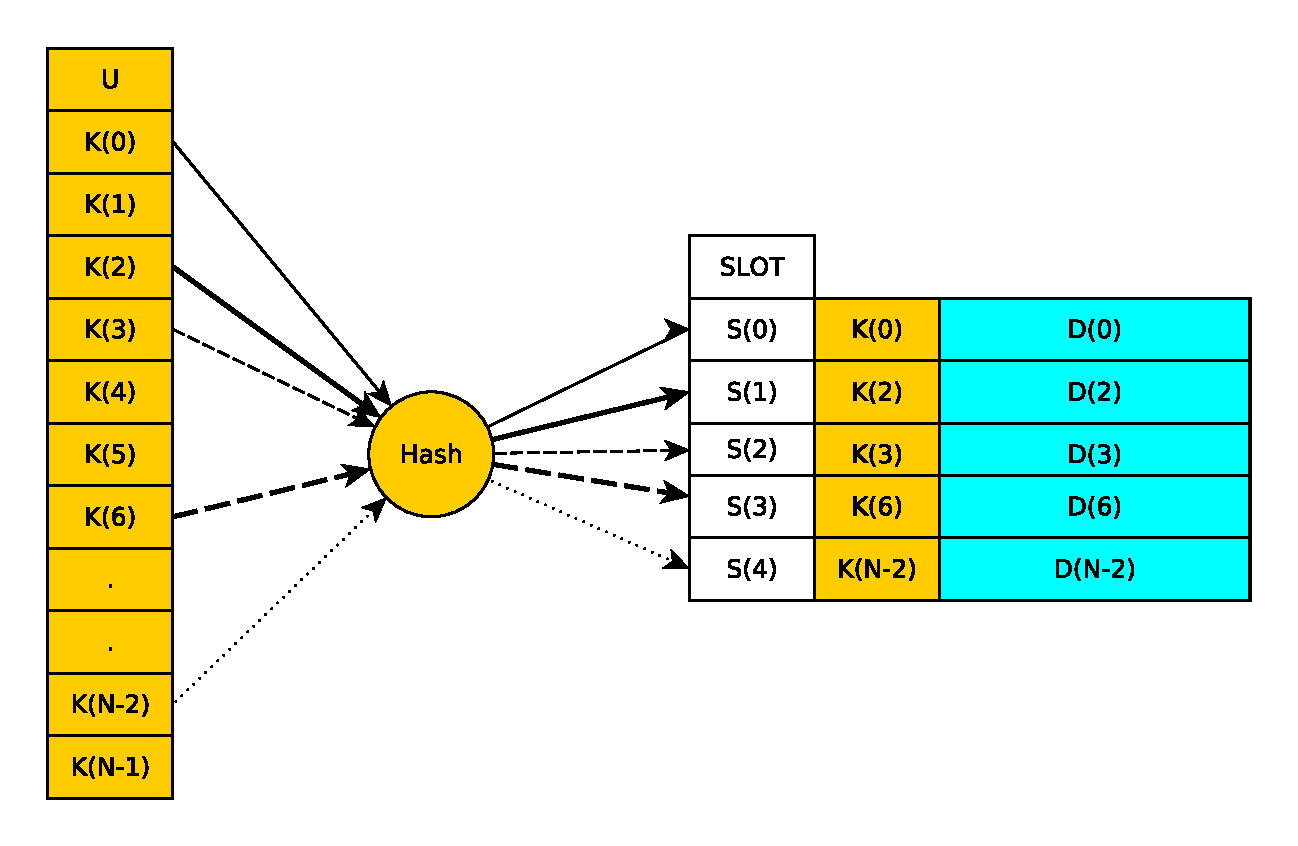
\includegraphics[scale=0.6]{fig/hash_table_example}	
	\caption{Princip fungování hašovacích tabulek}
	\label{fig:hash_table_example}
\end{figure}
%%%%%%%%%%%%% HASH TABLE EXAMPLE %%%%%%%%%%%%%%%
 
Vzhledem k tomu, že velikost tabulky je menší, než velikost univerza $|U|$,
budou nastávat kolize. Kolize je případ kdy, dva různé prvky univerza
$k_{1}, k_{2} \in U$ budou zobrazeny na stejný slot : 
$f_{hash} (k_{1}) = f_{hash} (k_{2})$. S tímto neduhem se dá vypořádat mnoha 
způsoby, jak uvidíme dále v sekci \ref{sec:collisions}.

\section{Kritéria kvality hašovacích funkcí}

Shrňme si nyní základní kritéria, která jsou důležiá pro hašovací funkce.

\subsection{Uniformní rozložení výstupů}

Pro dokonalé uniformní rozložení hašovací funkce bychom potřebovali \textit{náhodný}
generátor a i kdybychom nějaký měli k dispozici, pak by sice dobře dokázal 
rozprostřít jednotlivé prvky do hašovací tabulky, nicméně vzhledem k jeho náhodné 
povaze bychom je jen těžko zpět dohledávali. Musíme tedy zvolit jinou 
alternativu. Hašovací funkce musí být deterministická a musí dobře aproximovat
uniformní rozložení. Uniformní rozložení výstupů je předpokladem pro
nízkou časovou složitost hašovacích algoritmů, jak je vidět z příkladu
v sekci \ref{se:hash_function_design}.

\subsection{Odolnost proti kolizím}

Uvažujeme-li uniformní rozložení hašovací funkce, pak dva klíče u univerza
$U$ budou kolizní (dle \textit{birthday attack}) asi po $2^{\frac{m}{2}}$ 
operacích vložení\cite{NCHF_auto_design}. Pokud však hašovací funkce nebude
uniformě distribuovat výsledky, pravděpodobnost kolize se rapidně zvýší.

\subsection{Lavinový efekt}

Lavinový efekt (angl. Avalanche effect) je vlastnost hašovací funkce, při
které se rapidně mění výstup hašovací funkce pro malou změnu vstupu. 
Funkce které mají vysoký lavinový efekt mohou odolávat problému shlukování,
při kterém se některé části univerza mají tendenci shlukovat na výstupu
do skupin.

\subsection{Rychlost}

Nesporná výhoda hašovacích tabulek je jejich rychlost. Dobře navržená hašovací
tabulka dosahuje za určitých okolností složitosti $\theta (1)$. Pokud je však
výpočetní algoritmus příliš složitý, může daná funkce být pomalá. Je proto
nutné dbát na to, že příliš pomalý, i když dobrý algoritmus nemusí být
vždy ten nejlepší. 

\section{Návrh hašovací funkce}
\label{se:hash_function_design}

V praxi je často slyšet názor, že hašovací funkce pracují v konstantním čase.
To však není pravda, neboť výkon hašovací funkce záleží jednak na faktoru
zatížení hašovací tabulky a uniformnosti, s jakou dokáže hašovací funkce
přířazovat klíče do slotů.

Zaměřme se nejprve na zatížení tabulky a uvažme nějakou podmnožinu univerza
všech klíčů $K \in U$, hašovací tabulku $T$ s $m$ sloty a označme $n = |K|$.
Pokud $n$ bude menší než $m$, pak hašovací tabulka bude skutečně pracovat v 
$\theta (1)$, za předpokladu uniformního rozložení hašovací funkce. Pokud ale
bude $m$ menší než $n$, faktor zatížení bude větší než jedna a hašovací tabulka
v konstantním čase pracovat nebude. Uvažme $m=4$ a $n=5$. Pak za předpokladu
uniformního rozložení hašovací funkce, s vložením pátého prvku bude hašovací 
tabulka plná a nám nezbude než vkládaný prvek zařadit na začátek jednosměrně
vázaného seznamu.

Existuje mnoho metod pro konstrukci hašovací funkce, jako jsou například
\textit{metoda násobení}, \textit{metoda dělení} a další komplikovanější
přístupy. V současné době existují velmi dobré implementace obecných hašovacích funkcí.
Avšak žádná hašovací funkce nemůže pracovat pro všechna možná univerza stejně
dobře. Jako příklad uvažujme hašovací funkci navrženou metodou dělení :
$$ f_{hash}(k) = k \text{ mod } 8 $$ 
a dále uvažujme univerzum $U = \mathbb{N}$ a jeho
podmnožinu $K = \{1,2,3,4,8,13,22,71\}$, kterou budeme vkládat do tabulky.
Hašovací funkce je schopna uložit $8$ ruzných hodnot a v případě 
našeho výběru množiny $K$, se nám podaří uložit všechny, aniž by došlo ke kolizi.
Co by se ale stalo, pokud bychom byli omezení na univerzum pouze těch
přirozených čisel, která jsou dělitelné osmi $U = \{x \in \mathbb{N}
\land x \text{ mod } 8 = 0\}$? Nemohli bychom vybrat žádnou podmnožinu 
$F \in U$ takovou, kterou by funkce $f_{hash}$ nezobrazila pouze na jeden
slot.

Je vidět, že pokud máme informace o univerzu možných klíčů, můžeme navrhnout
hašovací funkci 'na míru' tak, aby měla lepší vlastnosti, než obecná
hašovací funkce. Tento úkol je však obtížný a neexistuj pro něj obecný
návod jak toho docílit. Musíme se spolehnout na zkušenosti, znalosti a v 
neposlední řadě také na intuici. Nebo můžeme zvolit úplně jiný přístup
jak napovídá kapitola \ref{sec:evolution_design}.

\subsection{Merkle-Damg\r{a}rdovo konstrukční schéma}
V oblasti kryptografických hašovacích funkcí se Merkle-Damg\r{a}rdovo schéma \cite{merkle0} jedním ze základních
stavebních kamenů moderních kryptografických hašovacích funkcí.
Dokazují to nesčetné implementace state of the art hašovacích funkcí na něm založené. Jako
přklad můžeme uvést algoritmy \textit{MD5} \cite{rfc1321}, \textit{SHA-1} \cite{rfc3174},
\textit{SHA-2} \cite{rfc4634} nebo \textit{Tiger} \cite{tiger}.

Jedná se o obecné schéma pro výstavbu hašovacích funkcí odolných proti kolizím z jednosměrně
kompresní funkce. Schéma se skládá z $n$ bloků pevné délky reprezentující vstupní zprávu.
K nim korespondují jednosměrné kompresní funkce. Každá kompresní funkce má na vstupu blok vstupních dat,
výstup předchozí kompresní funkce a produkuje výstup. Velikosti obou vstupu a výstupu jsou totožné,
proto nazýváme funkce kompresní. Poslední článek v řetězu kompresních funkcí představuje vhodné 
zarovnání. Někdy se také používá volitelna finalizační komponenta. Schéma blíže ilustruje obrázek 
\ref{fig:merkle_damgard}.

Bylo nezávisle ukázáno, že pokud je použitá vhodná 'vata'
(angl. \textit{padding}) pro zarovnání na správnou velikost a kompresní funkce jsou odolné
proti kolizím, pak vzniknuvší hašovací funkce je také odolná proti kolizím \cite{damgard0}.

Důvodem, proč se zde zabýváme kryptografickým schématem je, že jej používají i mnohé nekryptografické
hašovací funkce. I přes to, že tyto funkce nejsou kryptograficky bezpečné (což ani není účelem zavedení
Merkle-Damg\r{a}rdova shématu), použití kryptografického schématu dodá do hašovací funkce dodatečnou 
náhodnost. Použitím schématu docílíme v evolučním algoritmu značného zmenšení prohledávaného prostoru
a tedy lepší a rychlejší konvergence algoritmu viz. dále kapitola \ref{sec:evolution_design}.

Kromě Merkle-Damg\r{a}rdova schémata, exitují i jiná konstrukční schémata, například Merkleho strom 
\cite{merkle1}, často používaný v \textit{P2P} sítích,
struktura \textit{HAIFA} \cite{haifa} použitá v rodině kryptografických hašovacích funkcí \textit{BLAKE}
nebo funkce \textit{Sponge} \cite{sponge}. Těmito se zde však zabývat nebudeme.

\begin{figure}
	\centering
	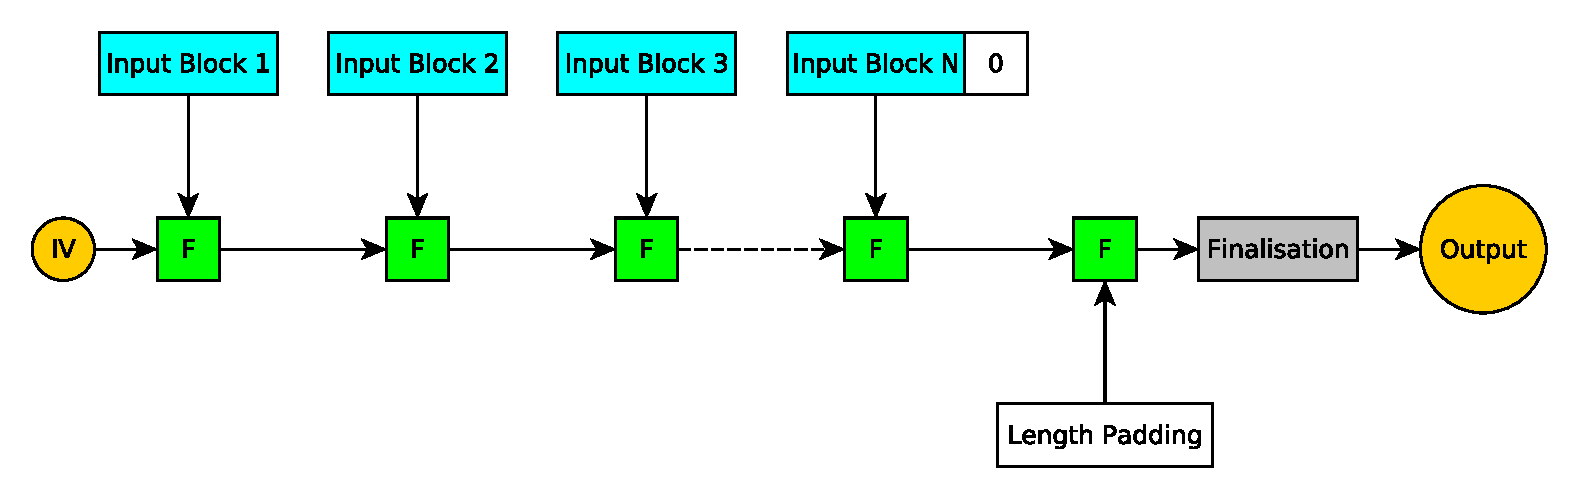
\includegraphics[width=\textwidth]{fig/merkle_damgard}
	\caption{Obecné Merkle-Damg\r{a}rdovo schéma pro $n$ bloků.}
	\label{fig:merkle_damgard}
\end{figure}

\section{Řešení kolizí při hašování}
\label{sec:collisions}

Situaci, kdy hašovací funkce zobrazí dva různé klíče na tentýž slot:
$f_{hash} (k_{1}) = f_{hash} (k_{2})$ nazýváme hašovací kolize nebo jen kolize. 
Kolize jsou nežádoucím důsledkem použití hašovacích funkcí
a chceme se jim pokud možno vyhnout, neboť zásadním způsoben negativně ovlivňují 
časovou složitost asociativních polí, které jsou na hašovacích funkcích postavené. 
Pro dobré pochopení kolizí je nezbytné uvést míru zaplnění hašovací tabulky
neboli takzvaný faktor zatížení $\alpha$ definovaný vztahem $\alpha = \frac{n}{m}$.
Právě časová složitost tabulky záleží za předpokladu uniformního rozložení 
hašovací funkce právě na \textit{faktoru zatížení}. 

Použitím kvalitní hašovací funkce můžeme riziko kolizí do jisté míry minimalizovat, ale
s narůstajícím faktorem zatížení $\alpha$ roste i riziko kolize, které dosáhne 
určitosti při $\alpha = 1$, tedy v hašovací tabulce není již žádný volný slot.
V takovém případě musíme kolizi vhodným způsobem řešit. Způsobů jak takovou sitaci
řešit je mnoho. My si v této sekci uvedeme ty, které jsou pro naši práci podstatné.

\subsection{Zřetězené hašování}

\begin{figure}
	\centering
	\begin{subfigure}[b]{0.49\textwidth}
		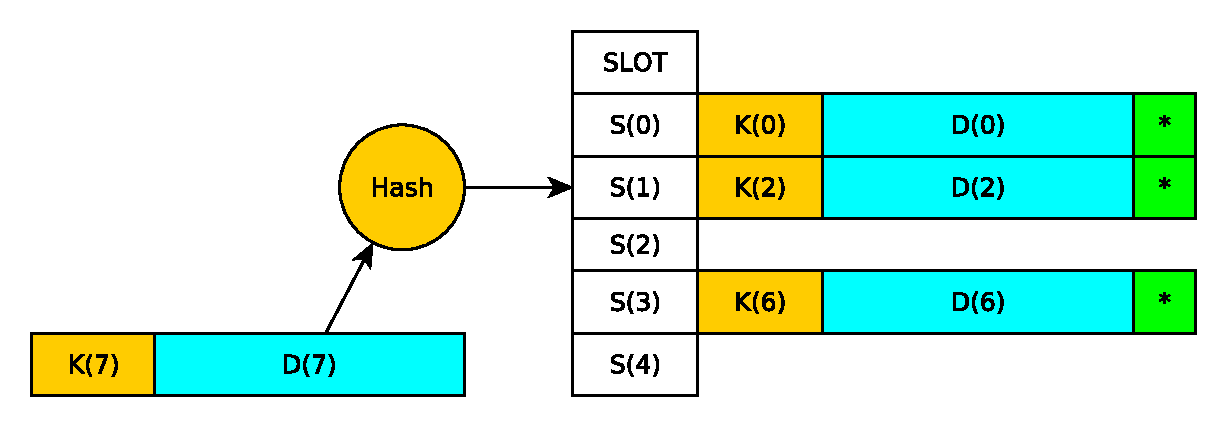
\includegraphics[width=\textwidth]{fig/chained_hashing_insert}
		\caption{Operace vložení nového prvku do hašovací tabulky způsobí kolizi klíčů.}
	\end{subfigure}
	\begin{subfigure}[b]{0.49\textwidth}
		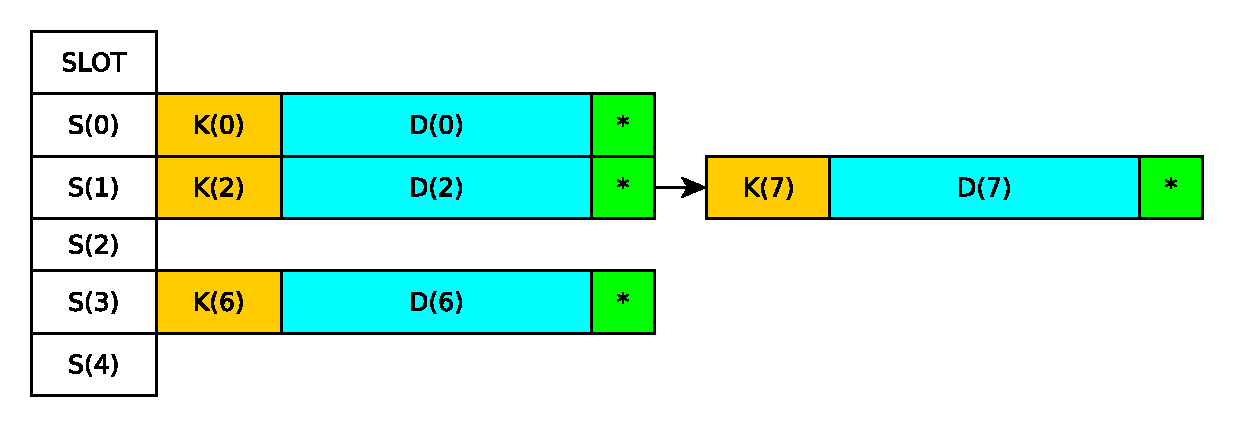
\includegraphics[width=\textwidth]{fig/chained_hashing_insert_result}
		\caption{Kolidovaná data se zřetězí v jednosměrně vázaném seznamu.}
	\end{subfigure}
	\caption{Demonstrace řešení kolize za použití vázaného seznamu.}
	\label{chained_hashing}
\end{figure}

Nejjednodušší a nejznámější formou řešení kolizí je řetězení dat v daném slotu. Jednotlivé 
sloty jsou reprezentovány jednosměrně vázaným seznamem, jehož položky tvoří data dohromady
s klíčem. Časová složiost takové implementace je:
\begin{itemize}
	\item v nejhorším případě $\theta (n)$, kdy všechny prvky budou namapovány
	na jeden slot,
	\item v průměru bude $\theta (1 + \alpha)$, za předpokladu
	uniformního rozložení, kdy pravděpodobnost namapování libovolného
	prvku na konkrétní slot je $\frac{1}{m}$.
\end{itemize}

Časovou složitost lze vylepšit vhodnou heuristikou, jakou může být například sledování
četnosti vyhledávání daných klíčů s následným vhodným přeuspořádáním jednosměrně vázaného
seznamu. Prostorová složitost této implementace také narůstá, neboť součástí každé položky jednosměrně
vázaného seznamu \textit{ll} je i ukazatel na další prvek potřebný pro získání
dalšího prvku seznamu \textit{next(ll)}. Řešení kolizí zřetězením kolidovaných 
položek do jednosměrně vázaného seznamu poskytuje za předpokladu uniformního rozložení dobré
výsledky a je výrazně rychlejší než samotný jednosměrně vázaný seznam. Existují však i jiné
přístupy, nabízející lepší vlastnosti.

\subsection{Kukaččí hašování}

Kukaččí hašování je moderní přístup k řešení hašovacích kolizí, za použití dvou a více hašovacích
funkci a dvou nebo více tabulek \cite{Cuckoo_hashing}. Častá implementace zahruje pouze jednu
tabulku, v níž má každá hašovací funkce vyhrazena vlastní prostor. Uvažujme univerzum klíčů $U$
a velikosti hašovací tabulky $m$. Pak na příklad pro dvě hašovací funkce 
$h_1, h_2$, kde $h_1 : U \rightarrow \{0,\ldots,r_1-1\}$ a $h_2 : U \leftarrow \{r_1,\ldots,r_2-1\}$ musí platit
$|\{0,\ldots,r_1-1\} \cup \{r_1,\ldots,r_2-1\}| = m$ a celkový počet slotů hašovací tabulky je $m$.

Opakem je implementace, kdy každá každá hašovací fukce obsluhuje dedikovanou tabulku. Zde pro
jiné dvě funkce $h_3, h_4$ tvaru $h_3 : U \rightarrow \{0,\ldots,r_1-1\}$ a $h_4 : U \leftarrow \{0,\ldots,r_1-1\}$
musí opět platit $|\{0,\ldots,r_1-1\} \cup \{0,\ldots,r_1-1\}| = m$. Tedy že hašovací funkce musí dokonale pokrýt
celou hašovací tabulku.

Název Kukaččí hašování je odvozen z chování některých druhů kukaček, kdy kukačky vytlačují vejce nebo své mladé
z hnízda. Toto chování je velmi podobné operaci vkládání. I přes to, že se rozhraní operace $Insert(S,x)$ nemění 
, výrazně se mění její vnitřní implementace. Operace vložení prvku do tabulky, vybere jednu z dostupných hašovacích
funkcí a pokusí se vložit prvek na příslušné místo. Dojde-li ke kolizi, původní prvek je vytlačen a nahrazen prvkem novým.
Vytlačený prvek je znovu vložen do tabulky, avšak za použití jiné hašovací funkce. Tento postup se opakuje tak dlouho, dokud
dochází při vkládání ke kolizím. Zřejmě tímto způsobem může docházet k cyklům. Maximální počet po sobě jdoucích vložení je tedy
omezen konstantou. Celý proces blíže demonstruje algoritmus \ref{alg:cuckoo_hashing} a obrázek \ref{fig:cuckoo_hashing}.

Podotkňeme, že není nezbytně nutné omezovat počet po sobě jdoucích vložení konstantou $MaxLoop$. Neúspěšnost je 
možné detekovat cyklením operace \Call{Insert}{}. Tu je možné modelovat v teoríí grafů jako bipartitní graf $G=(U,V,E)$, 
kde $U$ je množina vrcholú, zde slotů první hašovací tabulky, $V$ je opět množína vrcholů, zde slotů tentokrát však druhé
hašovací tabulky a $E \subset (U \times V) \cup (V \times U)$ je množina hran představující jednotlivá vytlačení původních
klíčů operace \Call{Insert}{}. Pak platí následující tvrzení:
\begin{itemize}
	\item Klíč $x \in U$ nelze do hašovací tabulky vložit, jestliže souvislá komponenta grafu indukovaná operací
		\Call{INSERT}{} $G$ obsahuje dva a více cyklů
		\cite{standford1}. 
	\item Naproti tomu Klíč $x \in U$ lze do hašovací tabulky vložit, jestliže souvislá komponenta grafu indukovaná operací
		\Call{INSERT}{} $G$ obsahuje žadný
		a nebo maximálně jeden cyklus \cite{standford1}.
\end{itemize}
Přesto omezení konstantou $MaxLoop$ může být vhodné z několika důvodů. Jedním z důvodů je zjednodušení celého algoritmu
další pak nárůstající výpočetní a paměťová náročnost (složinosti se nemění), kterou s sebou nese detekce cyklu.

\begin{figure}[!ht]
	\centering
	\begin{subfigure}[b]{0.53\textwidth}
		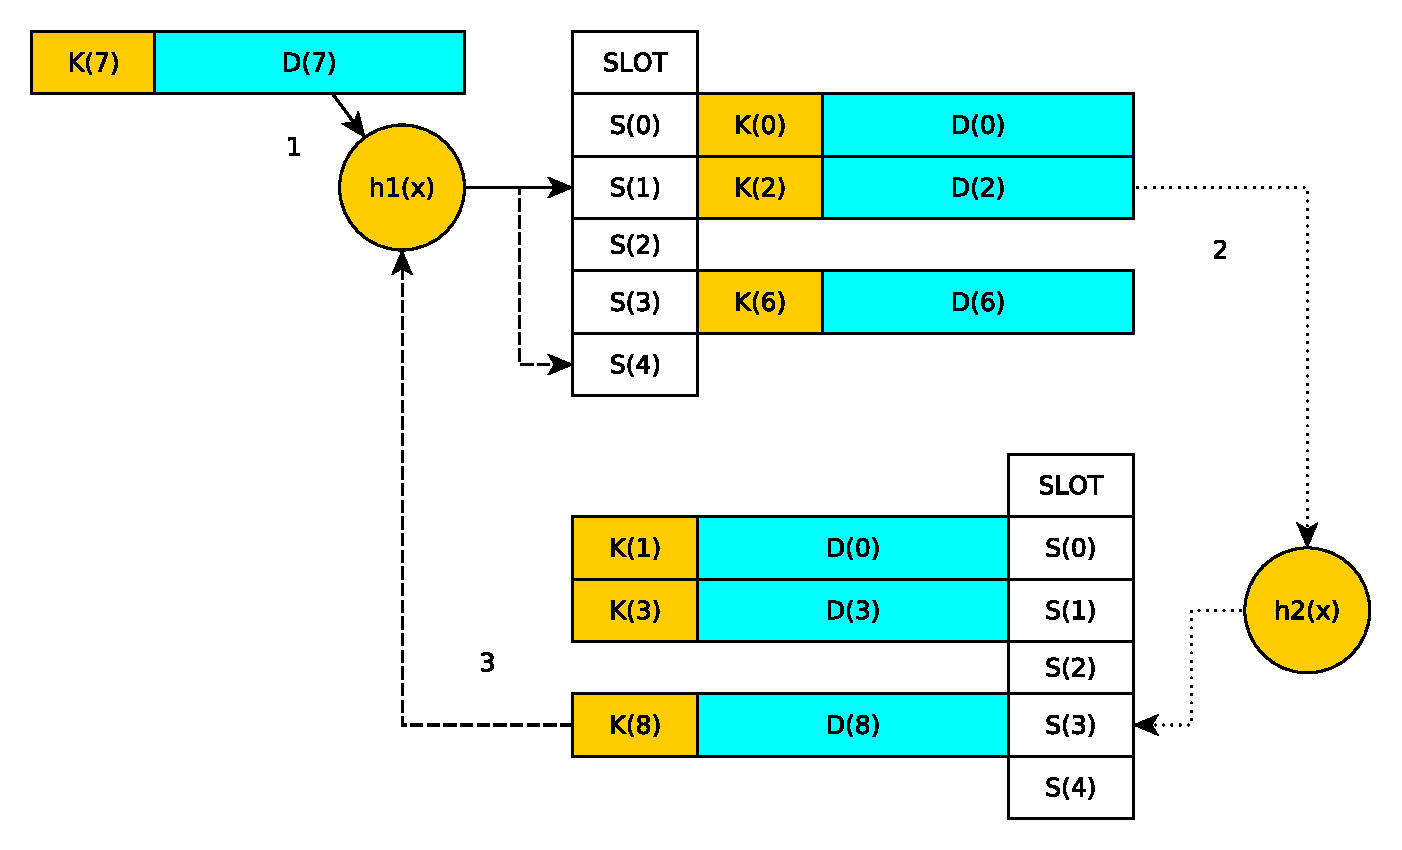
\includegraphics[width=\textwidth]{fig/cuckoo_hashing_insert}
		\caption{Kolize je řešena za použití druhé hašovací funkce.}
	\end{subfigure}
	\begin{subfigure}[b]{0.46\textwidth}
		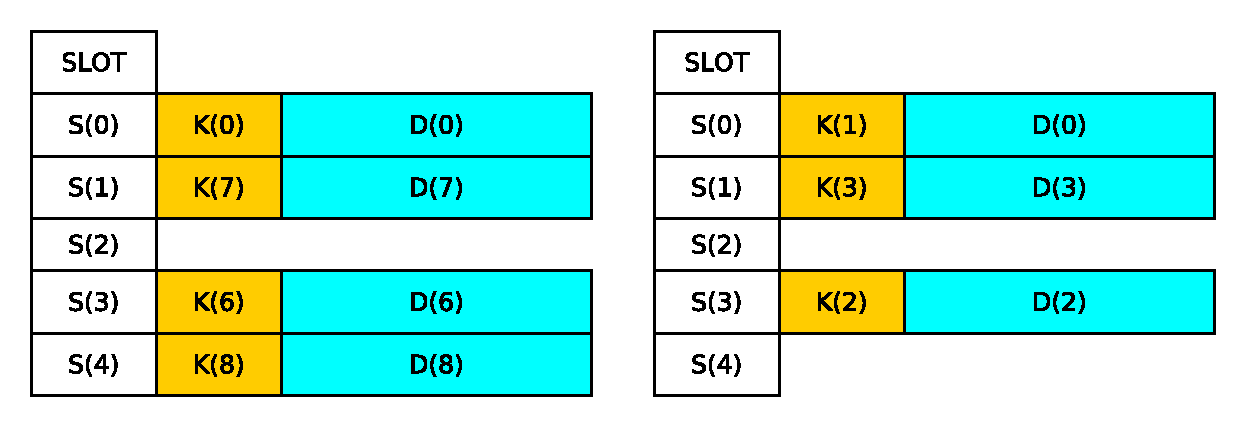
\includegraphics[width=\textwidth]{fig/cuckoo_hashing_insert_result}
		\caption{Data v tabulkce se po několikanásobném vytlačení ustálí.}
	\end{subfigure}
	\caption{Demostrace řešení kolize za použití kukaččího hašování.}
	\label{fig:cuckoo_hashing}
\end{figure}

Pokud v průběhu operace dosaženo mezní hodnoty $MaxLoop$, předpokládejme tedy, že jsme narazili na cyklus. V takovém případě 
provedeme nejprve operaci \Call{rehash}{} a poté zkusíme prvek vložit opětovným zavoláním funkce \Call{insert}{x}.
Funkce \Call{rehash}{} zajišťuje, aby při opětovném vložení prvku do tabulky znovu nevzniknul cyklus. Toho se dá
dosáhnout například použitím jiných hašovacích funkci \cite{Cuckoo_hashing}. Není třeba znovu vytvářet hašovací tabulku,
postačí hašovací tabulku projít a na každý prvek uplatnit nejprve operace \Call{delete}{x}, která jej z tabulky odstraní 
a následně jej znovu vložit za použití operace \Call{insert}{x}.

\begin{algorithm}
\begin{algorithmic}
\Function{insert}{x}
	\Repeat
		\State $x \leftrightarrow T_1[h_1(x)]$
		\If {$x = \bot$} \Return \EndIf
		\State $x \leftrightarrow T_2[h_2(x)]$
		\If {$x = \bot$} \Return \EndIf
	\Until{$!MaxLoop$}
	\State \Call{rehash}{}; \Call{insert}{x}
\EndFunction
\end{algorithmic}
\caption{Pseudokód popisující operaci $insert$ za použití kukaččího hašování.}
\label{alg:cuckoo_hashing}
\end{algorithm}

Časová složitost výhledávání v tabulce za použití Kukaččího hašování je v průměru $\theta(1)$. Pro nás je ale
důležitější, že časová složitost v nejhorším případě zustává také konstantní. Je však důležité zohlednit 
následující faktory:
\begin{itemize}
	\item Je nutné použít takové hašovací funkce, které dobře uniformě distribuují svoje výstupy. Pokud by tento
	předpoklad nebyl splněn, může být (a pravděpodobně bude) často volána nákladná operace \Call{REHASH}{}.

	\item Operace \Call{REHASH}{} nezvětšuje ani nezmenšuje kapacitu hašovací tabulky. Vzhledem k tomu, že každý slot
	hašovací tabulky pojme právě jeden klíč, maximální faktor zatížení $\alpha$ je právě roven jedné (což je přesný
	opak chování zřetězeného hašování, kdy za použití vázaného seznamu snadno dosáhneme $\alpha \geq 1$).

	\item Je dobré počítat s tím, že i za použití více hašovacích funkcí se koeficientu $\alpha = 1$ přiblížíme jen
	vzdáleně. Opětovné pokusy o vložení prvku do tabulky, která má již koeficient $\alpha \approx 1$ nevyhnutelně
	vyústí ve volání funkce \Call{REHASH}{}. Je tedy vhodné podrobit Kukaččí hašování nějaké formě heuristiky, kdy
	bude její kapacita ve vhodný okamžik zvětšena, aby nedocházelo k opakovanému volání funkce \Call{REHASH}{}.
\end{itemize}

\section{Analýza existujících řešení}
Cílem této sekce je podat přehled o existujících state of the art obecných hašovacích funkcích, protože některými z těchto
funkcí budeme porovnávat námi navržené hašovací funkce. Také budeme analyzovat, z jakých elementárních operací se 
dané hašovací funkce skládají, což nám poslouží především pro návrh množiny funkcí dále viz. kapitola  
\ref{sec:solution_design}. Nejprve se zaměříme na krátký popis vybraných hašovacích funkcí a poté na samotný rozbor.

\begin{itemize}
	\item \textit{MurmurHash2} \cite{murmurhash2} je druhou funkcí z rodiny hašovacích funkcí \textit{Murmur} vytvořenou
		Austinem Appleby v roce 2008. Tato funkce se těší velké oblibě mezi hašovacími experty. V průběhu let se však 
		ukázalo, že trpí závažnou bezpečnostní chybou zahlcení hašovací funkce (angl. \textit{Hash-Flooding}), kdy správnou
		volbou hašovaných klíčů dojde ke klastrování výstupů na jeden slot. Tato chyba má za následek extrémní zpomalení 
		hašovací tabulky vystavěné nad touto funkcí a odepření služby (angl. Denial-of-Service) celé aplikace. 
		
		Tato hašovací funkce je použita v mnohých \textit{open-source} projektech, mezi něž patří i Apache Hadoop. 
		
	\item \textit{MurmurHash3} \cite{murmurhash3} je již třetím pokračovatelem funkcí z rodiny \textit{Murmur}. Dle
		autora se v nové generaci jedná o rychlejší a robustnější funkci. Je postavena na stejném základu a nese si 
		s sebou jednoduchost a dobré výkon stejně jako předchozí verze. Bohužel stále trpí výše zmíněnou bezpečnostní
		chybou.
	
	\item \textit{CityHash} \cite{cityhash_slides} je rodina hašovacích funkcí, primárně určená pro hašování řetězců. 
		Vznikla ve společnosti Google (Geoff Pike a  Jyrki Alakuijala, 2011) a je silně optimalizována pro použití na
		hardwaru, který se nachýzí v datacentrech
		společnosti Google. Je inspirována funkcemi z rodiny \textit{Murmur}. Funkce vnáší do problematiky
		netradiční přístup spočívající v použití více než jedné aritmetické operace ve většině kroků. O funkci je známo,
		že trpí stejnou zranitelností jako předchozí dvě funkce, jimiž se inspirovala.
	
	\item I přes svůj nesporný přínos byla funkce \textit{CityHash} již o tři roky později nahrazena novou rodinou
		hašovacích funkcí \textit{FarmHash} \cite{farmhash} \cite{Simone2014}. Opět za ní stojí společnost Google. Její primární aplikací
		jsou opět datacentra společnosti Google, ale tentokrát byl kladen důraz také na rychlost a především
		uživatelskou vstřícnost a snadnou použitelnost na přenosných zařízeních jako jsou mobilní telefony a podobně.
	
	\item V případě funkce \textit{lookup3} \cite{NCHF_auto_design} se jedná o velmi známou a kvalitní funkci, vytvořenou Robertem Jenkinsem
		již v roce 2006. Jedná se o o state-of-the art hašovací funkci, což dokazují aplikace v produktech firem
		Google, Oracle nebo Dreamworks. Hašovací funkce se rovněž objevila v některých implementacích \textit{open-source}
		projektů mezi něž patří \textit{PostgreSQL}, \textit{Linux}, \textit{Perl} nebo \textit{Ruby}.
	
	\item \textit{SuperFastHash} \cite{Hsieh2004-2008}. Jedná se o populární hašovací funkci, kterou vytvořil Paul Hsieh (2004 - 2008). Dle autora je použita
		v projektu \textit{WebKit}, důležité součásti webových prohlížečů Safari a Google Chrome. Funkce byla také součástí
		některých verzí bývalého produktu \textit{Flash Player} firmy \textit{Macromedia}. Při vývoji byl kladen
		důraz na vysokou míru lavinového efektu a rychlost. 
		
	\item \textit{SpookyHash} \cite{Jenkins2012} je další funkce vytvořená Robertem Jenkinse mv roce 2011. Její doménou by měla být dle autora
		rychlost a vyniká v lavinovém efektu. 
\end{itemize}

Výše zmíněné hašovací funkce lze považovat za state-of-the art hašovací funkce. Jsou vytvořeny největšímy odborníky v daném
oboru s praxí přesahující někdy i desítky let. Většina z nich je použita v projektech velkého významu, ať už se jedná o
projekty s otevřeným zdrojovým kódem či o uzavřené projekty. Námi navržené hašovací funkce budeme chtít s těmito
funkcemi srovnat a ukázat tak, relevantnost (či nerelevantnost) našich výsledků.

Zaměřme se nyní na to, které elementární operace jsou využívání v těchto hašovacích funkcích. Tato informace nám pomůže se
zorientovat v problematice návrhu a umožní nám dobře zvolit funkce i terminály v námi navržených hašovacích funkcí. Některé
hašovací funkce pracují nejen s elementárními hašovacími funkcemi, ale i s jejich vysokoúrovnovými kombinacemi. Tyto
takzvané \textit{mixovací komponenty} nebudeme chápat jako samostatné operace, ale rozložíme je v naší analýze na
elementární operace. Pro lepší orientaci v problematice poslouží přehledová tabulka \ref{tab:generic_hashes_analysis}.
Rozbor byl prováděn z referenčních implementací, které jsou všechny kromě funkce \textit{FarmHash} obsaženy v balíku
\textit{SMHasher} \cite{appleby2016}. Oficiální referenční implementace funkce \textit{FarmHash} je možné získat z repozitáře na
stránce \textit{Github} \footnote{https://github.com/google/farmhash/blob/master/src/farmhash.cc}. Implementace hašovacích
funkcí obsahují opravdu široké spektrum operátorů. Nás budou zajímat pouze ty, které jsou použity pro samotnou tvorbu
výstupu. Nesmí nás tedy zmást například použití logického součtu nebo součinu v řidících konstrukcích nebo operace
sčítání a odčítání použíté pro krokování vstupu po blocích určité velikosti. 

Ve zdrojových kódech referenčních implementací jednotlivých hašovacích funkcí můžeme vidět některé opakující se vzory.
Vždy je použita jedna nebo více aritmetických operací. V našem výběru se vždy jedná o sčítání ($+$) , násobení  ($*$) nebo
jejich společnou kombinaci. Další nedílnou součástí dobré hašovací funkce je volba posunu nebo rotace. Většína vybraných
funkcí spoléhá na rotace, menšina poté na posuny. Najdou se i takové implementace, které používají obě dvě, ale za
primární operaci lze považovat jen rotaci. Posuny jsou v takovém případě použity jako součást vysokoúrovňové 
\textit{mixovací komponenty}.

\begin{table}[!ht]
	\centering
	\begin{tabular}{lccccccccccc}
		\hline
		Operace            & $*$ & $/$ & $+$ & $-$ & Posuny & Rotace & AND & OR & XOR & $\neg$ & Konstanty \\
		\hline
		MurmurHash2   & \checkmark & & & & \checkmark & & & & \checkmark & & \checkmark \\
		MurmurHash3   & \checkmark & & \checkmark & &  & \checkmark & & & \checkmark & & \checkmark \\
		lookup3              & & & \checkmark & \checkmark & & \checkmark & & & \checkmark & & \checkmark \\
		FarmHash         & \checkmark & & \checkmark & & \checkmark & \checkmark & \checkmark & & \checkmark & & \checkmark  \\
		CityHash          & \checkmark & & \checkmark & & \checkmark & \checkmark & & & \checkmark & & \checkmark \\
		SpookyHash     & & & \checkmark & & & \checkmark & & & \checkmark & & \\
		SuperFastHash & & & \checkmark & & \checkmark & & & & \checkmark & & \\
		\hline		
	\end{tabular}
	\label{tab:generic_hashes_analysis}
	\caption{Analýza existujících hašovacích funkcí z pohledu použitých elementarních operací.}
\end{table}

Další skupinu často používaných operací tvoří operace logické a bitové. Zde v drtivé většíně narazíme na operaci XOR. Zřídka
používanou operací je logický součin (AND). Naopak nikdy nejsou použity operace logického součtu (OR) a jedničkového
doplňku ($\neg$). Poslední skupninou jsou konstanty. Ty jsou použity pro přivedení dodatečné náhodnosti do hašovací funkce.
Často se jedná o prvočísla, která svými specifickými vlastnostmi netrpí na shlukování výstupu. Setkáme se však i s jinými 
konstantami, jako například konstanta \texttt{0xdeadbeef} použitá v případě funkce \textit{lookup3}.

\chapter{Evoluční návrh}
\label{sec:evolution_design}

% Chapter INTRO
Evoluční návrh je netradiční disciplína, která využívá evoluční algoritmy
k návrhu. Evoluční algoritmy spadají do oblasti umělé 
inteligence. Specifickou vlastností mnoha úloh spadajících do obasti umělé 
inteligence je, že často vhodným způsobem prohledávají prostor $U$,
reprezentující všechna možná řešení (kandidátní) dané úlohy 
\cite{evolution_hardware}. Evoluční algoritmy se dají považovat za speciální metodou 
prohledávání prostoru kandidátních řešení.

% Section Natural computing
\section{Počítání podle přírody}
\label{sec:natural_computing}
Počítání podle přírody (Natural computing) je sohrný termín pro tvorbu 
inteligentních strojů napodobováním biologických procesů, chování živých 
tvorů nebo jejich mechanismů. Řadíme sem také výpočetní paradigmata, která 
svoji inspiraci nalezla v přírodních procesech nebo použití organismů a 
jiných netradičních materiálů jako výpočetních platforem. Míra do jaké je 
přírodní fenomén napodoben se různí. Od Téměř úplného napodobení až po 
inspiraci. 

Jedním z motivů pro vznik alternativních výpočetních přístupů a počítání 
podle přírody je lepší splynutí s reálným světem a jeho probémy.
V tomto kontextu je vhodné zmínit \textit{soft-computing}. \textit{Soft-computing}
je podmnožinou počítání podle přírody, bývají sem zařazovány 
neuronové sítě, \textit{Support Vector Machines}, fuzzy systémy, evoluční 
algoritmy a teorie chaosu. Postupy spadající do \textit{Soft-computing} 
tolerují nepřesnosti a nejistotu čímž dosahují vysoké robustnosti a 
lepšího vztahu s realitou. Počítání podle přírody ve svůj prospěch používá 
procesy zejména fylogeneze, ontogeneze a epigeneze. Fylogeneze označuje proces
evoluce druhů, ontogeneze proces vývoje mnohobuněčného organismu a epigeneze
je nějaký proces, který nastává v již složitějším organismu 
(sem řadíme například neuronové sítě).
Dále se se počítání podle příody inspirovalo procesy vznikajícími ve společnosti, 
v usuzování jedinců apodobně. My se zde budeme zabývat hlouběji pouze fylogenezí, neboť 
právě na ní je založena myšlenka evolučních algoritmů.

\section{Evoluční algoritmy}

Fylogeneze je proces evoluce druhů. Evoluce je umožněna schopností reprodukce jednotlivých
jedinců, kdy potomkové se od svých rodučů liší jen velmi málo. Při reprodukci však dochází také
k náhodným občasným mutacím, které zabezpečují dostatečnou diferzitu a vzniká tak nový
genetický materiál. Na fylogenezi jsou založené evoluční algoritmy. 

Evoluční algoritmy lze chápat jako speciální optimalizační metodu nad prostorem 
$$U = D_{1} \times D_{2} \times D_{3} \times \ldots \times D_{n}$$
všech kandidátních řešení. Takový prostor je pak kartézský součin domén, kde
jednotlivé domény univerza mohou nabývat
hodnot z předem známých, často nějak omezených intervalů \cite{evolution_hardware}.  

V matematické optimalizaci, bychom se snažili hledat hodnoty $x \in U$ takové,
pro které je hodnota účelové funkce
$$ f : U \to \mathcal{R} $$
minimální (hledání maxima lze úpravou účelové funkce převést na hledání minima).
Minima mohou být globální nebo lokální, ostrá nebo neostrá. Řešíme tedy úlohu,
kdy hledáme nějaký argument, jehož hodnota účelové funkce spadá do množiny optimálních
hodnot účelové funkce \cite{nlprog}.
$$ argmin_{x}\{f(x)|x \in U\} $$		
V kontextu evolučních algoritmů nazýváme $f$ funkcí \textit{fitness} a nehledáme 
argument $x$, pro nějž je funkce $f$ minimální, ale postačuje nám najít argument $x$ 
takový, že $f(x)$ splní nějaké předem dáné ukončovací podmínky.

\subsection{Princip}
Evoluční algoritmy jsou inspirované procesem reprodukce jedinců napříč generacemi.
Na začátku výpočtu algoritmu vytvoříme počáteční populaci $P_{0}$, tj.
populaci generace nula o předem známé velikosti $n$.
Volba jedinců do počáteční populace jsou různé, můžeme například sáhnout po náhodném 
výběru nebo volit jedince za použití vhodné heuristiky.

%$$ \mathcal{P}_{0} = \{x|x \in U \land vyber\_do\_počáteční\_populace(x) \} $$

V každém dalším kroku evolučního algoritmu, který nazýváme generace, je nejprve vybráno
$m$ vhodných jedinců z generace předchozí $P_{t - 1}$, kteří nám tvoří množinu rodičů. Aplikací
genetických operátorů nad množinou rodičů vznikne množina potomků, Následně se z obou
množin vybere nová generace $P_{t}$ o velikosti $n$ a celý process (znázorněn na diagramu \ref{fig:eaflow})
se opakuje. Způsoby výběru rodiču jsou různé stejně
tak jako možné genetické operátory. Oběma se budeme zabývat později.

%%%%%%%%%%%%% EVOLUTION ALGORITHM FLOWCHART %%%%%%%%%%%%%%%
\begin{figure}[!ht]
	\centering
	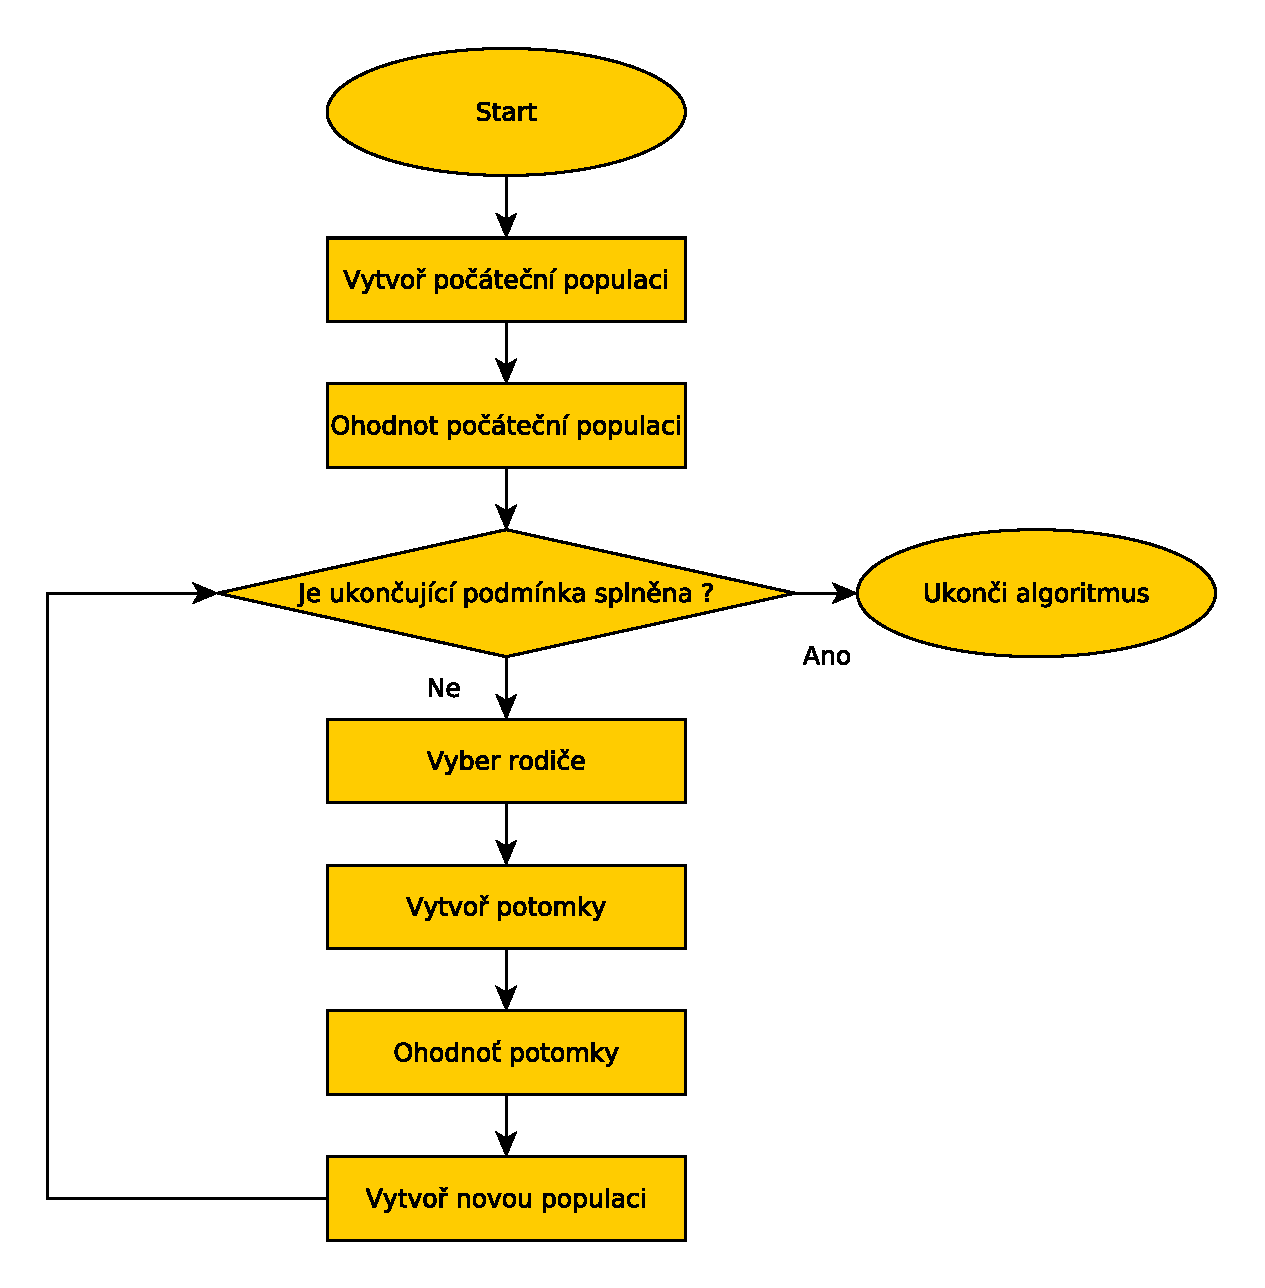
\includegraphics[scale=0.4]{fig/evolution_algorithm_flowchart}	
	\caption{Obecný postup výpočtu evolučního algoritmu}
	\label{fig:eaflow}
\end{figure}
%%%%%%%%%%%%% EVOLUTION ALGORITHM FLOWCHART %%%%%%%%%%%%%%%

\subsection{Fitness funkce}
Fitness funkce je obdoba účelové funkce z oboru matematické optimalizace. Název fitness
pochází z oboru evoluční biologie, kde hodnota fitness popisuje biologickou zdatnost jedince
\cite{evolution_hardware}. Vstupem fitness funkce je (v jednodušším případě) jedinec
reprezentovaný chromozomem a výstupem je hodnota reprezentující zdatnost jedince.

Ve složitějších případech je nutné rozlišovat mezi prostorem genotypů a fenotypů. Genotypem
nazýváme v kontextu evolučních algoritmů prostor všech možných řešení, tedy 
všech možných chromozomů. Fenotyp je soubor charakteristik, projevů a chování,
jimiž se daný jedinec reprezentovaný určitým chromozomem projevuje.
Zobrazení z prostoru genotypů do prostoru fenotypů lze potom vyjádřít následovně:
$$ f_{phenotype} : U \to \mathcal{F}, $$
Potom je však nutné modifikovat naši fitness funkci následovně :
$$ f : \mathcal{F} \to \mathcal{R} $$
a celý proces evaluace jedince bude poté kompizice těchto dvou funkcí :
$$ f_{eval} = f \circ f_{phenotype}$$

Volba potažmo návrh vhodné fitness funkce je značně obtížná. Neexistuje žádný obecný
předpis pro jejich návrh. Musíme se spoléhat na obecná pravidla, zkušenosti nebo 
intuici. Velké množství dobře zakomponovaných informací o problému ve fitness funkci je
dobrým základem pro úspěšný evoluční algoritmus. Obecně tedy platí, že 
vhodně zvolená fitness funkce má značný dopad na kvalitu výsledného řešení.

\subsection{Způsoby selekce}
Způsoby selekce jsou důležitým faktorem při návrhu evolučního algoritmu. Selekce
je proces, při němž se vybýrají rodiče z aktuální populace určení k reprodukci. 
Dobrý selekční algoritmus musí být schopen upřednostňovat jedince s vysokou hodnotou
fitness funkce, na druhou stranu musí zajistit dostatečné množství genetického 
materiálů pro dalši generace. Často využívané selekční mechanismy, zejména v kontextu
genetických algoritmů jsou například \cite{selection_schemes_comparison} :

\begin{itemize}
	\item \textit{deterministická selekce}, kde se do množiny rodičů vybere $k$
		jedinců z aktuální populace s nejvyšší hodnotou fitness,
		
	\item \textit{proporcionlní selekce}, kde pravděpodobnost výběru jedince $i$ je 
		rovna vztahu $p_{i} = \frac{f(i)}{\sum_{j=1}{N} f(j)}$,
		
	\item \textit{turnajová selekce}, kdy je v několika kolech turnaje postupně 
		porovnáno několik náhodně vybraných jedinců a vítěz turnaje je zařazen
		do množiny rodičů. Turnaj provedeme $n$-krát, kde $n$ je požadovaná mohutnost
		množiny rodičů. 
\end{itemize}

\subsection{Genetické operátory}
Evoluční algoritmy využívají křížení i mutaci, oba mechanismy jsou převzaty z
oboru buněčné biologie, kde se uplatňují v procesu redukčního dělení buněk.

Operátor mutace se aplikuje na potomka
a vytvoří z něj potomka mutovaného. Stejně jako v biologii, mutace se vyskytuje
pouze v malém počtu případů. Našim cílem je prozkoumat prostor $U$ postupně a
konvergovat k dobrým řešením. V případě vysoké pravděpodobnosti mutace se již
nejedná o algorigmus \textbf{evoluční}, nýbrž \textbf{revoluční} a algoritmus připomíná 
spíše náhodné prohledávání. Operátor mutace je velmi důležitý, neboť zanesení
náhodne mutace zajišťuje nový genetický materiál, čímž je algoritmus jednou za
čas nucen prozkoumat vzdálenější bod prostoru. Neuvázne tak v lokálních extrémech.

Při křížení dochází k přenosu částí chromozomů rodičů na potomka. Způsobů křížení
existuje celá řada. Obecně však platí, že způsob křížení je závislý na zvolené 
reprezentaci. Pokud máme jedince reprezentovaného grafem, operátor křížení 
se bude značně odlišovat od případu, kdy máme jedince reprezentovaného binárním
vektorem. 

Uveďmě si zde alespoň nejznámější druhy křížení nad binární reprezentaci, jimiž jsou:
\begin{itemize}
	\item \textit{jednobodové křížení}, kdy se určí místo křížení určující,
		která část chromozomu doputuje do potomka.
		
	\item \textit{dvoubodové křížení} je obdobou výše zmíněného, avšak pro dva body
		křížení a
	\item \textit{uniformní křížení}, které je do značné míry zobecněním výše zmíněných.
		 Určí $n$ genů v chromozomu, jejichž hodnoty jsou vystřídány.
\end{itemize}

\subsection{Návrh evolučního algoritmu}

Kvalita námi navrženého evolučního algoritmu, je zejména závislá na následujících faktorech:
\begin{enumerate}
	\item reprezentace problémů a jeho kódování,
	\item použitá fitness funkce,
	\item zobrazení z prostoru genotypů do prostoru fenotypů,
	\item volbou genetických operátorů a způsoby selekce,
	\item nastavením parametrů genetického algoritmu.
\end{enumerate}

Prostor každého problému řešitelného evolučnímy algoritmy je jiný. Neexistuje tedy obecný
evoluční algoritmus, který by kvalitně řešil všechny problémy. Toto tvrzení podporuje takzvaný
\textit{No Free Lunch} teorém. Pokud uvážíme dostatečně velký počet optimalizačních problémů,
neexistuje žádný optimalizační algoritmus, který projde každý bod prostoru $U$ právě jednou
a v průměru bude efektivnější než ostatní optimalizační algoritmy \cite{nflteorem, evolution_hardware}. 
Z tohoto tvrzení plyne, že chceme-li řešit optimalizační problém skutečně efektnivně, musíme 
do našeho evolučního algoritmu \textbf{vložit co nejvíce informací} o problému prostřednictvím 
zejména položek zmíněných výše.

\subsection{Genetické algoritmy}

Evoluční algoritmy popisují množinu algoritmů, jejichž činnost je určena procesem Darwinovské
evoluce. Na druhé straně je však neomezuje natolik, aby se od sebe nemohly (někdy i velmi
významně) lišit.

Asi nejvýznamějším žástupcem evolučních algoritmů jsou genetické algoritmy. Jedinci jedné populace
jsou reprezentovány řetězcem (chromozomem) binárních, celočíselných nebo i reálných hodnot.
Iniciální populace vzniká buď náhodně nebo za použití vhodné heuristiky. Uplatňují se zde všechny
běžné selekční mechanismy a stejně tak zde najdeme použity všechny druhy metod křížení.
Mutace se taktéž používá. Nevýhodou mohou někdy být chromozomý pevné délky.

\subsection{Evoluční strategie}

Dalším zajímavým algoritmem jsou evoluční strategie. Jejich největší zajímavostí je, že
se spoléhají pouze na operátor mutace. Křížení se zde nevyskytuje. Nové generace se zde
vytvářejí zejména tak, že rodičovská populace je mutována přičtením hodnoty normálního rozložení s nulovou
$x' = x + \mathcal{N}(0, \sigma)$
střední hodnotou. Rozptyl $\sigma$ se mění na základě toho, jak dobře algoritmus aktuálně
konverguje. Jako selekční mechanismy se užívá totální elitismus ve variantách $(\mu + \lambda)$
a $(\mu, \lambda)$ \cite{ES}. Uvažujeme-li $\mu$ množinu rodičů a $\lambda$ množinu jejich
potomků, pak :

\begin{itemize}
	\item $(\mu + \lambda)$ vybere do další generace nejlepší jedince z množiny
		rodičů a potomku
	\item $(\mu, \lambda)$ vybere do další generace jen ty nejlepší potomky. Rodičovská
		generace tedy vymírá.
\end{itemize} 

\section{Genetické programování}

Pro naší práce je zejména zajímavé genetické programování, neboť právě to jsme zvolili 
jako evoluční algoritmus pro řešení našeho problémů. Seznámíme se s ním podrobněji a 
proto mu věnujme celou sekci.

Genetické programování je speciálním druhem evolučního algoritmu, kde jednotlivce a 
celé populace tvoří počítačové programy. Výpočet iterativně transformuje počítačové
programy na jiné počítačové programy aplikací genetických operátorů, které jsou 
pro genetické programování specifické. Výstupem genetického algoritmu
je v případě, že uspěje, nějaký program. 

\subsection{Reprezentace}
Evolvované programy musíme vhodně reprezentovat. Musíme pří tom klást důraz na to,
že programy je mezi sebou třeba křížit, mutovat a obecně na nich provádět nutné
genetické operace. Na druhé straně však chceme volit takovou reprezentaci, která
nám umožní programy evaluovat, tudíž vykonávat je nad zadaným vstupem. 

Jedinci v populaci jsou reprezentování raději jako \textit{abstraktní syntaktické stromy}
\cite{GPTutorial} než jako řádky programu. Ukázka jedince v geneticém programování je na
diagramu \ref{fig:exampletree1} a zobrazuje jedince reprezentovaného programem
\texttt{max(min(x,y), 5 + z)}. Stromy se skládají z uzlů a listů. Listy jsou
reprezentovány terminálním symbolem z množiny terminálů $T$ a uzly jsou reprezentovány
funkcí z množiny $F$. Na diagramu \ref{fig:exampletree1} množinu funkcí tvoří 
$F = \{max, min, +\}$ a množinu terminálu $T = \{5, x, y, z\}$. Množiny povolených
funkcí a terminálů dohromady tvoří primitivní množinu systému. Prostor možných 
řešení můžeme tedy definovat jako množinu všech možných stromů, které mohou vzniknout
kombinací funkcí a terminálů :

$$ U = \{t | t=(FT)^{n}, 0 \leq n \leq max\_depth \}$$

Programová reprezentace stromů se liší v závislosti na použitém programovacího jazyku.
Platí však, že 
v prosředích náročných na výpočetní výkon je paměťová náročnost grafové reprezentace
neefektnivní. Stromové reprezentace lze užít i nepřímo za použití prefixové notace.
Pří použití prefixové notace se závorky stanou nadbytečnými a program lze v paměti
uložit jako \textit{lineární sekvenci symbolů}. Jako příklad poslouží diagram 
\ref{fig:exampletree1}, tedy \texttt{max min x y + 5 z}. Volba reprezentace tedy
v konečném důsledků záleží na uživateli a jeho preferencích, požadavcích a prostředí. 

%%%%%%%%%%%%% TREE REPRESENTATION EXAMPLE 1 %%%%%%%%%%%%%%%
\begin{figure}[!ht]
	\centering
	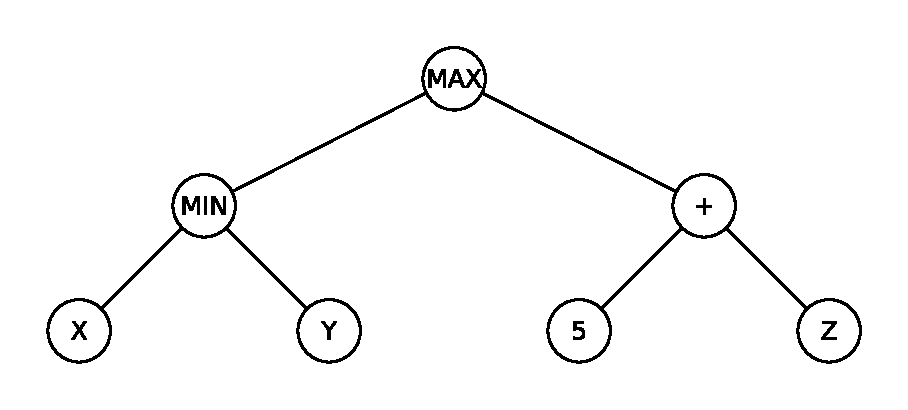
\includegraphics[scale=0.6]{fig/example_tree1}	
	\caption{Ukázka reprezentace programu max(min(x,y), 5 + z)}
	\label{fig:exampletree1}
\end{figure}
%%%%%%%%%%%%% TREE REPRESENTATION EXAMPLE 1 %%%%%%%%%%%%%%%

\subsection{Inicializace nulté populace}

Pro inicializaci nulté populace platí obecná pravidla. Můžeme ji buď volit náhodně
nebo použít nějakou vhodnou heuristiku. Je zde však specifická vlastnost, kterou 
musíme vzít do úvahy. Naše programy nemají pevně omezenou velikost (délka
chromozomu je proměnná). Jak velké náhodné programy tedy generovat? Existují tři
základní přístupy:

\begin{enumerate}
	\item \textit{Full} metoda, kdy náhodně vygenerujeme strom do maximální povolené
		hloubky,
	\item \textit{Grow} metoda, generujeme stromy proměnlivé délky a tvaru (maximální
		hloubka je omezena) a
	\item \textit{Ramped half-and-half}, kdy polovina populace je generována metodou
		\textit{Grow} a druhá metodou \textit{Full}, za proměnlivé maximální hloubky.
\end{enumerate}

Metoda Full vždy a za všech okolností generuje plné stromy. V uzlech jsou funkce
vybírány náhodně z množíny $F$ a jakmile algoritmus dosáhne maximální hloubky,
nageneruje terminály z množiny $T$ a skončí.

Grow metoda naproti tomu generuje v uzlech s určitou pravděpodobností i terminály, čímž
je schopna vytvářet stromy různých délek i tvarů. Je však velmi závisla na velikostech
množin $F$ a $T$. Pokud $|T| << |F|$ algoritmus degraduje na metodu Full. Pokud
na druhé straně $|T| >> |F|$, algoritmus bude generovat jen velmi malé stromy.

Aby se omezil dopad rozdílných velikostí množin $T$ a $F$, John Koza navrhl alternativu
v podobě algoritmu ramped half-and-half. Ten používá obě metody současně na polovinu 
jedinců populace a maximální hloubku stromu volí náhodně, čímž zajišťuje proměnlivou
velikost i tvar stromů.

\subsection{Genetické operátory a selekce}

V případě selekce do množiny rodičů, se využívají všechny běžné selekční mechanismy
známé z evolučních algoritmů, avšak nejčastěji se využívá turnajová selekce následovaná
proporcionální selekcí.

Zajímavější je to v případě genetických operátorů křížení a mutace. Nejčastější formou
křížení je \textit{podstromové křížení}. U rodičů vybraných k reprodukci se se náhodně 
vybere bod křížení, který v genetickém programování zastupují větve stromu. Potomek
vznikne umístěním podstromu prvního rodiče na prázdnou větev druhého rodiče (rodiče
implicitně zachováváme). Celý proces blíže ilustruje diagram \ref{fig:tree_crossover}

%%%%%%%%%%%%% TREE CROSSOVER EXAMPLE 1 %%%%%%%%%%%%%%%
\begin{figure}[!ht]
	\centering
	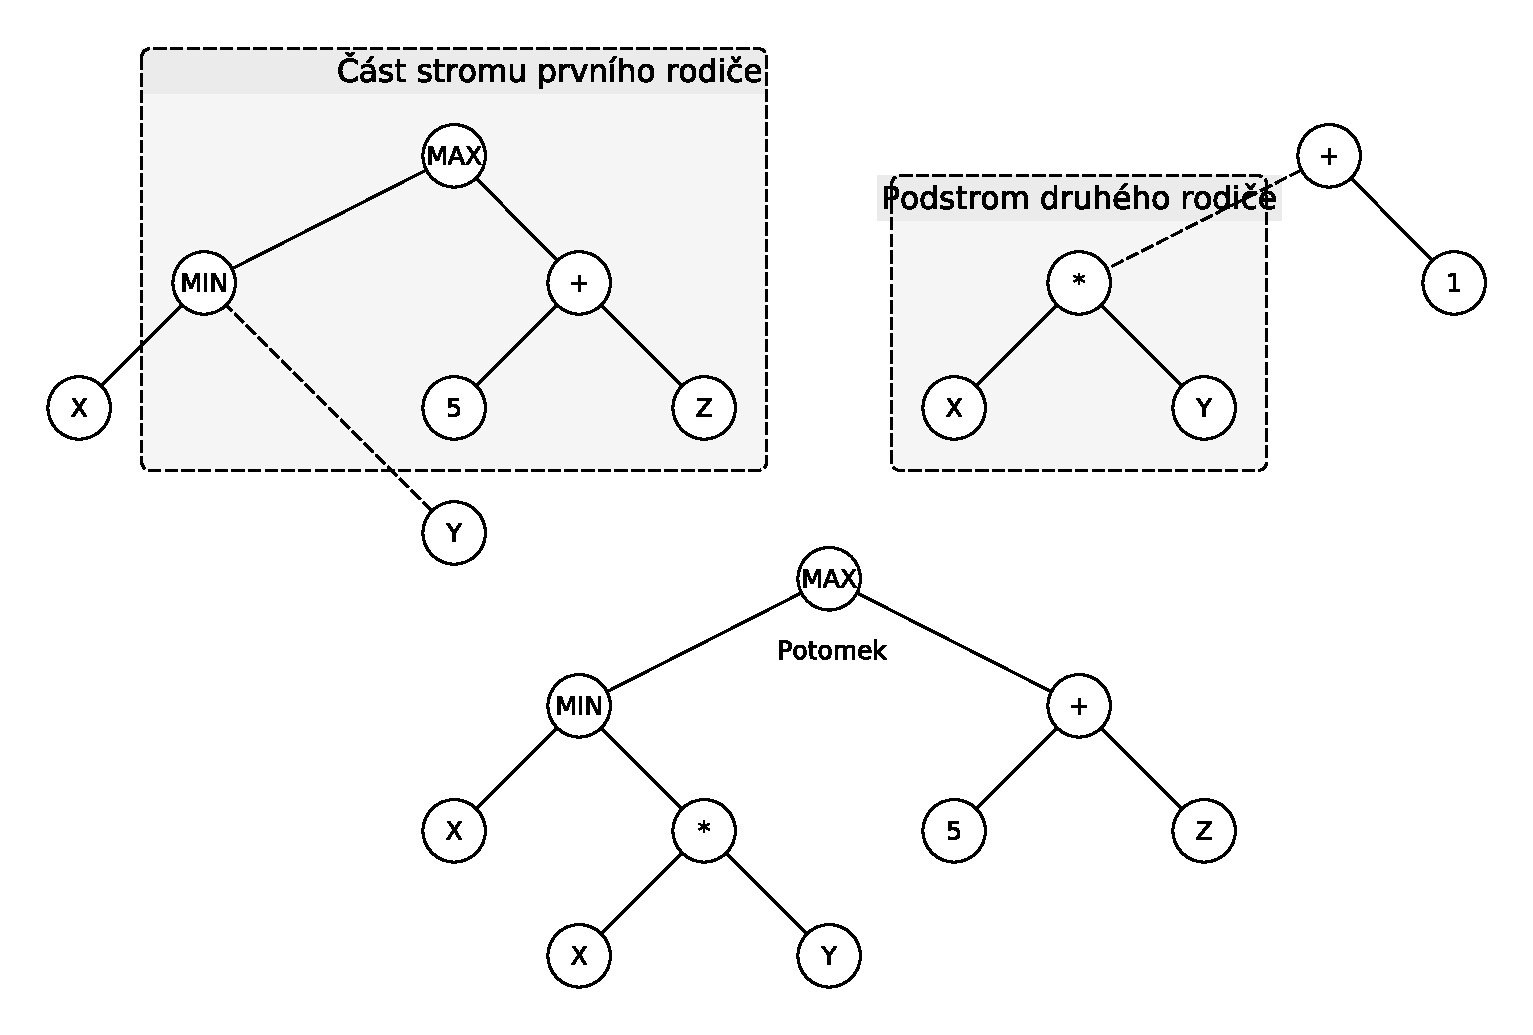
\includegraphics[scale=0.6]{fig/tree_crossover}	
	\caption{Ukázka operátoru podstromového křížení}
	\label{fig:tree_crossover}
\end{figure}
%%%%%%%%%%%%% TREE CROSSOVER EXAMPLE 1 %%%%%%%%%%%%%%%

Je vidět, že křížení vytvoří pouze jednoho potomka. Pro více potomků celý proces 
opakujeme. Dale existuje specializace podstromového křížení, obdoba jednobodového
křžení, kdy se určí v obou rodičích stejný bod křížení a přehození korespondujících
podstromů. Je však potřeba oba strommy projít a najít společný region, tedy část stromu,
kde je možné křížit. Existují další varianty jako je křížení se zachováním kontextu, 
velikost zachovávající křížení a uniformní křížení. Těmito se zde zatím blíže zabývat
nebudeme.

Nejběžnější druh mutace je podstromová mutace. Algoritmus podstromové mutace ve stromu
náhodně zvolí větev z níž náhodně vygeneruje nový podstrom, jak ilustruje diagram
\ref{fig:subtree_mutation}. V případě tohoto algoritmu jde v podstatě o alternativu k
podstromovému křížení s jedním rodičem a jedním náhodně generovaným stromem.

Další variantou mutace v genickém programování je uzlová nutace, kdy na každý
uzel stromu je s určitou nizkou pravděpodobností mutace aplikována. Staré uzly
se nahrazují novými se stejnou aritou.

%%%%%%%%%%%%% SUBTREE MUTATION EXAMPLE 1 %%%%%%%%%%%%%%%
\begin{figure}[!ht]
	\centering
	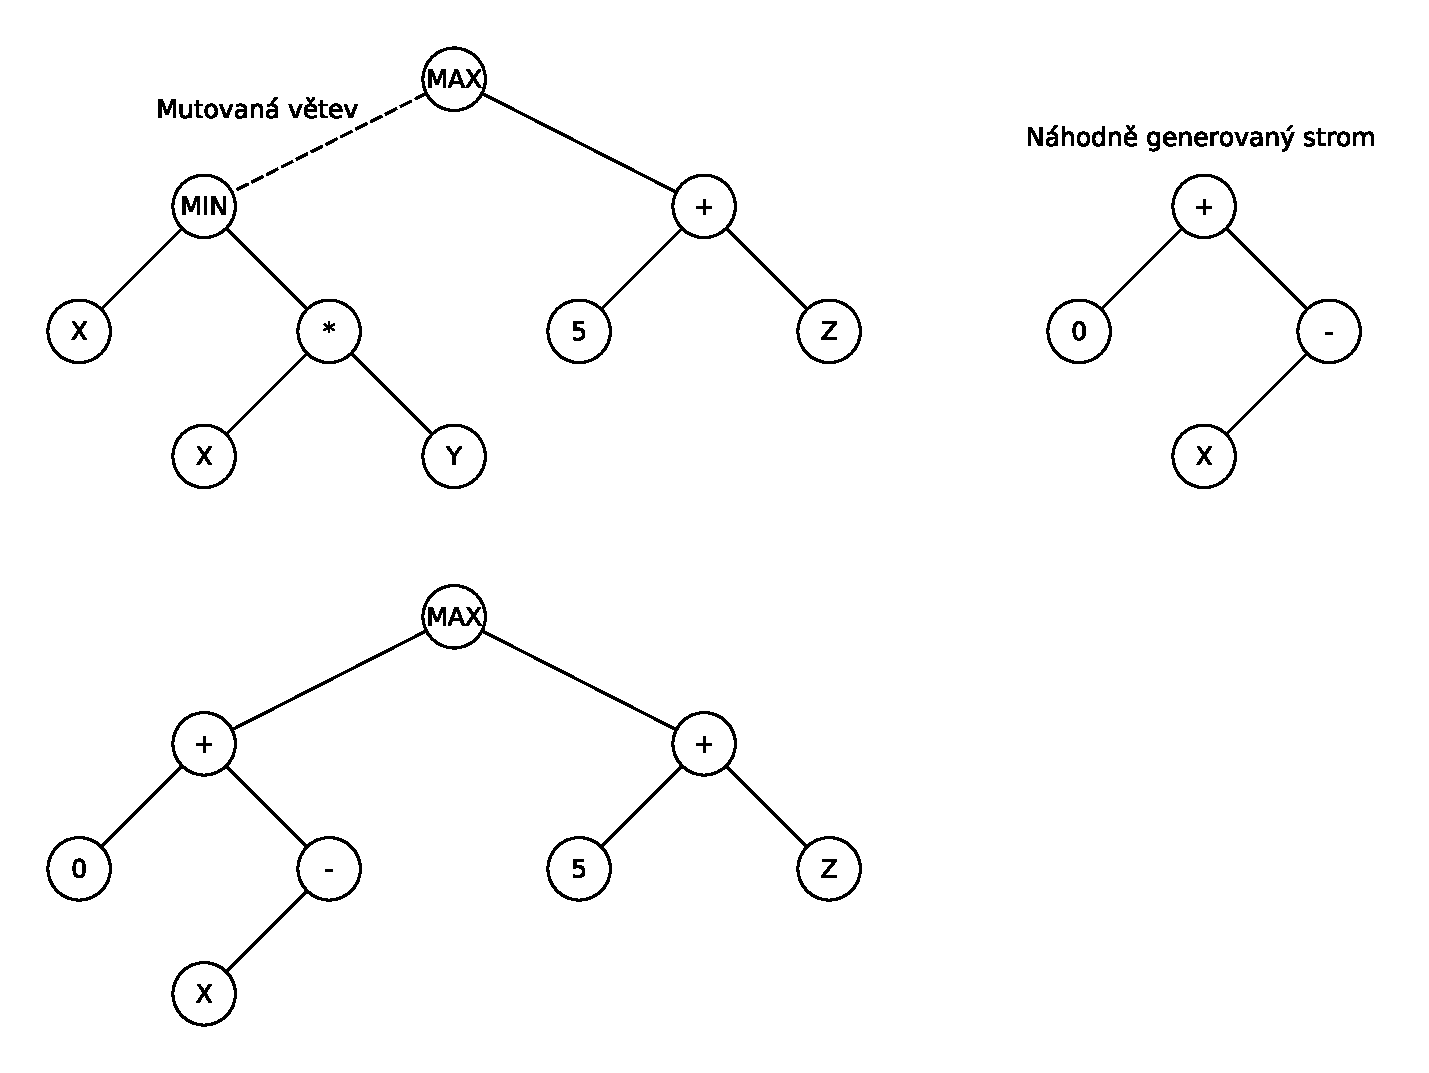
\includegraphics[scale=0.6]{fig/subtree_mutation}	
	\caption{Ukázka operátoru podstromové mutace}
	\label{fig:subtree_mutation}
\end{figure}
%%%%%%%%%%%%% SUBTREE MUTATION EXAMPLE 1 %%%%%%%%%%%%%%%

\subsection{Fitness funkce}
Populace v genetickém programování jsou programy. Evaluace kvality programu se provádí
zpravidla spuštěním daného programu nad daným vstupem a ohodnocením výstupu. Spuštění 
programu nad zadaným vstupem můžeme chápat jako zobrazení z množíny genotypů do množiny
fenotypů za vstupu dalšího parametru. Celý proces evaluace může být tedy chápán jako :
$$ f_{eval} = f \circ f_{run}(input)$$
kde $f$ je standarní fitness funkce a $f_{run} : I \to (U \to \mathcal{F})$ je
modifikované zobrazení genotyp-fenotyp pro nějaký vstup $I$.

Fitness funkce v případě genetického programování se liší od té tradiční v jednom
důležitém směru. Protože pracujeme nad programy, musíme poskytnout způsob, jak daný
program spustit. Možností by bylo program zkompilovat. To s sebou nese značnou režii
a tak toto řešení není v mnoha případech vhodné. Pokud však bychom daný program chtěli
evaluovat několikrát (mnohokrát), může se i toto řešení jevit jako vhodné.

Častější je ale programy interpretovat, to znamená projít strom od listů ke kořenu a 
spočítání hodnoty uzlu za vstupu hodnot jeho následníků. Kostru algoritmu bude jistě
tvořit průchod \textit{postorder}. Evaluace jednotlivých hodnot však nemusí být za všech 
okolností triviální, může například nastat případ, kdy bude program dělit nulou nebo
se snažit sečíst hodnoty různých typů (např. \texttt{Bool} a \texttt{Int}). Při reprodukci
jedinců zde narážíme na podobné problémy jako například v teorii typů. Typovost se v
případě genetického programování řeší dvěma základnímy způsoby:

\begin{enumerate}
	\item \textit{typová unifikace}, kdy veškeré uzly i listy stromu budou téhož typu,
	\item \textit{silná typovost}, kdy součástí každého uzlu i listu stromu bude uveden
	explicitně jeho typ.
\end{enumerate}

Typová bezpečnost je nutná zejména kvůli operátoru křížení a mutace. V prvním případě
musíme tedy počítat s tím, že jakýkoli podstrom může být zavěšen jako argument
libovolné funkci z množny $F$ a výsledný program přesto musí být interpretovatelný.
Jinými slovy navratový typ libovolné funkce z množiny $F$ musí být stejný jako
typ libovolného vstupního argumentu jakékoli dostupné funkce. Toho můžeme dosáhnout
například jednoduše tím, že všechny funkce z množiny $F$ budou definovány nad jedním
oborem hodnot totožného typu. Často to však není možné, proto se musíme někdy uchílit
například k implicitním typovým konverzím.

Druhou možností je použití silně typovaných stromů. Tento způsob je obecnější, neboť
nám umožňuje použít naprosto libovolnou množinu funkcí $F$. Je však také výrazně
implementačně složitější. Veškeré reprodukční operace zde musí provádět explicitní
typovou kontrolu a častokrát dlouho procházet strom, než naleznou uzel vhodný ke 
křížení či mutaci. To má dopad samozřejmě hlavně na časovou složitost, která je 
vyšší než v případě typové unifikace.

Společnou vlastností, kterou je nutné splnit jak v případě silné typovosti, tak v případě
typové unifiace je, abychom se vypořádali s možnými
nedefinovanými hodnotami, které jsou typické pro vstupy některých parciálních funkcí
jako je dělení, kde hodnota je nedefinovaná pokud je dělitel roven nule.
S parciálními funkcemi se můžeme vypořádat tím, že je explicitně rozšíříme na funkce
totální nebo v případě, je-li nedefinovaná hodnota detekována, značně snížíme jedincův 
fitness.

\chapter{Návrh metod pro evoluční návrh hašovacích funkcí}
\label{sec:solution_design}

Jak již bylo řečeno v kapitole \ref{sec:hashing}, navrhujeme-li hašovací funkci ``na
míru'' nějakému konkrétnímu univerzu klíčů, můžeme dosáhnout podstatně lepší 
výkonnosti hašovací funkce, než je tomu v případě obecných hašovacích funkcí.

\section{Definice problému}
Našim problémem bude navrhnout konkrétní hašovací funkci pro hašování domény
\texttt{IP} adres. Adresa \texttt{IP} je číslo, jednoznačně identifikující síťové
rozhraní v síti, která používá internetový protokol \texttt{IP}. Vzhledem k tomu,
že budeme hašovat čísla, nabízí se otázka, zda by nebylo vhodné použít tabulku
s přímým přístupem, tedy použít \texttt{IP} adresy pro přístup do tabulky
přímo bez využití hašování. Bohužel neznáme konkrétní interval nebo podmnožinu
univerza \texttt{IP} adres a celé univerzum je příliš velké na to, aby jeho 
prvky mohly sloužit jako čísla slotů do tabulky. Ve verzi 4 se jedná o 32 
bitové číslo a verzi 6 dokonce o velikosti 128 bitů. Tabulka by tedy musela
mít $2^{32} = 4 294 967 296$ slotů v případě  \texttt{IP} verze 4 a ve verzi 6
dokonce $2^{128} \approx 3 \times 10^{38}$
slotů. Je vidět, že tabulky by byly opravdu velké a jejich paměťová náročnost
by byla nedostupná i pro specializované počítače, uvažujeme-li, že by takový
stroj měl dělat i něco jiného, než uchovávat tak ohromnou tabulku. Musíme se
tedy uchílit k návrhu hašovací funkce.

Pracujeme nad čtyřmi datasety, kde každý dataset obsahuje právě 8192 různých 
IP adres. Pro každý dataset bude nutno navrhnout zvláštní hašovací funkci a tu
na dané vstupy ``natrénovat''. Nenavrhujeme obecnější hašovací funkci, která by dobře
pracovala nad libovolnou podmnožinou celého univerza IP adres, ale velmi
specifické funkce, které budou dobře pracovat právě nad zvoleným datasetem.
Protože celý hašovaný prostor je předem znám, snažíme se najít takové hašovací
funkce, které pojmou co nejvíce z dané podmnožiny. State-of-the-art řešení je v
tomto případě taková hašovací funkce, která pojme celý podprostor, její 
faktor zatížení bude roven právě jedné ($\alpha = 1$). Taková řešení však
bude těžké najít. Pro naše účely postačí, nalezneme-li takové, které budou
pracovat lépe, než obecné hašovací funkce, vytvořené člověkem. Je zde samozřejmě
možnost použít metody perfektního hašovaní \cite{perfect_hashing}, ale to nemusí
být ve všech případech například z důvodů použití na specializovaném hardware
dostupná možnost. Zabývat se jí tedy nebudeme.

\section{Princip}
Hašovací funkce budeme navrhovat evolučními algoritmy, a to konkrétně za použití 
genetického programování, popsaného v předchozí kapitole \ref{sec:evolution_design}.
Zvoleno bylo genetické programování, protože 
jedince populace reprezentuje abstraktními syntaktickými stromy. Jenotlivé syntaktické 
stromy budou reprezentovat přímo hašovací funkce a ty budeme interpretovat nad zadanými vstupy.
Ohodnocení konkrétního jedince bude spočívat v nahašování jednoho celé subsetu a na výstupu budeme
měřit počet kolizí, tedy kolik různých klíčů zobrazilo kandidátní řešení na stejný slot.

\section{Přinos práce}
Evoluční návrh hašovacích funkcí se ukázalo jako zajímavé téma v posledním 
desetiletí \cite{dobai0,NCHF_auto_design,grammar_evolution,safdari}.
Naprostá většina prací se se zaměrovala na návrh obecných hašovacích
funkcí. Byly použity jak evoulční návrh tak evoluční optimalizace. Jedna z prací
podobná té naší je \cite{safdari}. Je podobná ve smyslu cíle a použité techniky,
avšak autor zde použil evoluční optimalizaci namísto návrhu. Autor optimalizuje
parametry $a,b$ následující hašovací funkce:
$$h_{a,b}(k) = ((ak + b) \; mod \; p) \; mod \; N$$
kde $p$ je nějaké prvočíslo a $N - 1$ je největší index slotu hašovací tabulky.
``Výsledky jsou slibné, ale použitá metodika je sporná'' \cite{NCHF_auto_design}.
Protože množina klíčů obsahuje celá čís	la a je volena náhodně (pseudonáhodně), náskýta se otázka,
proč vůbec evolvovat hašovací funkci, když mohou být použity její prvky k indexování
napřímo. Druhá věc je, že autor používa jako primární metriku fitness funkce odolnost
vůči kolizím, která je silně závislá na vstupní množině. Funkce tedy nemusí dobře 
zobecňovat.

Vhodnější metrikou pro návrh obecných hašovacích funkcí je lavinový efekt, který 
není závislý na vstupu. Tohoto faktu využili autoři další podobné práce \cite{NCHF_auto_design}
zabývající se návrhem hašovacích funckí. Tato práce je pravděpodobně nejblíže té 
naší ale s rozdílem, že my nenavrhujeme obecné hašovací funkce. Autoři stejně jako my,
zvolili genetické programování jako evoluční platformu a volili i podobné parametry.
Jako základ pro svoji fitnes funkci zvolili lavinový efekt, který není
závislý na vstupu. Funkce navržené jejich systémem otestovali na různých vstupních třídách
a dosáhli slibných výsledků. Tvrdí, že jeji algoritmus je velice robustní, protože změny
klíčových parametrů mají jen velmi nízký nebo žádný dopad na výsledné funkce. Bohužel
součástí jejich experimentu není porovnání s algoritmem náhodného prohledávání, ke 
kterému mohl jejich systém nedopatřením degradovat a který je z povahy věci také 
velmi robustní. Autoři také tvrdí, že evolučně navrhují hašovací funkce, což 
vzhledem k tomu, že navrhují kompresní funkce Merkle-Damg\r{a}rdova schémata
není ůplně pravda. Takový přístup se nachází na pomezí evolučního návrhu a optimalizace.

Zajímavou prací, která se vydala přístupem kartézského genetického programování je
\cite{dobai0}. Kartézské genetické programování je zejména vhodné pro aplikace blízké
hardwarové vrstvě, takže jeho volba se zdá velmi dobrá vzhledem k cílové aplikační doméně,
kterou jsou síťové prvky. Nesporný přínos práce spočívá v použití Kukaččího hašování, které
je použito za účelem zvýšení faktoru zatížení výsledné hašovací tabulky a práce tak dosáhla velmi
dobrých výsledků. Faktor, který tato a naše práce sdílí je návrh doménově specifické hašovací 
funkce, kde hašovanou doménou jsou také \texttt{IP} adresy. Práce se však rozchází zejména ve volbě 
fitnes funkce. Zatímco my (jak uvidíme později v této kapitole) jsme zvolili přístup, kdy hašujeme
celý daný rozsah a měříme výskyt kolizí, autoři měří počet úspěšně nahašovaných adres až do výskytu
první kolize. Taková metrika je vskutku zajímavá, ale intuitivně se naskýta úvaha, že fitnes funkce
velmi špatně ohodnotí řešení, která mají kolizi velmi brzo, ale přitom mohou nahašovat velkou část
celého rozsahu. Fitnes funkce jasně míří na cíl nahašovat celý rozsah (tedy optimální řešení), toho
nicméně nedosáhla. Bude zajímavé porovnat výsledky naší prace s s výsledky dosaženými v této
práci. Autoři opět používají Merkle-Damg\r{a}rdovo schéma a práce se tudíž také nachází na 
pomezí evolučního návrhu a evoluční optimalizace.

\section{Návrh fitness funkce}

V naší práce navrhujeme specifickou
hašovací funkci pro specifické univerzum hodnot. Proto můžeme použít jako kritérium
kvality odolnost vůči kolizím, které je nepřímým ukazatelem toho, jak dobře funkce
náhodně distribuuje své výstupy. Evaluovanou hašovací
funkci budeme testoat nad všemi prvky univerza. To znamená, že budeme navrhovat
celkem ctyři hašovací funkce, pro každý vsupní dataset jednu. Kdybychom pro všechny čtyři
datasety navrhovali jednu jedinou, nedostali bychom dobré výsledky. Výsledná hašovací tabulka
by měla 8192 slotů, ale byla by ``natrénována'' nad všemi adresami ze všech datasetů, které mají dohromady mnohem více 
různých klíčů. Navic 
bychom se museli zabývat vhodnou volbou trénovacích dat, což je obtížný úkol a navíc přídat
kritérim, které by bralo v úvahu zobecňování. Výsledná hašovací funkce by již nebyla čistě jednoúčelová, ale
někde ``na půl cesty'' mezi obecnou a velmi specifickou hašovací funkci.

Neméně důležitým kritériem je rychlost hašovací funkce a to obzvláště v aplikacích jako jsou
síťové směrovače nebo jiná uplatňění náročná na rychlost a odezvu. Jak uvidíme později v této
kapitole, veškeré námi navržené funkce jsou implicitně rychlé, protože explicitně omezíme hloubku
abstraktních syntaktických stromů a vhodně zvolíme množinu terminálů a neterminálů. 

\section{Zvolené parametry genetického programování}

V této sekci uvedeme, jaké parametry jsme zvolili parametry pro geneticé programování.

\subsection{Genetické operátory a metoda selekce}

Jako operátor mutace použijeme podstromovou verzi podstromovou mutaci. Jedná se o základní formu mutace
u genetického programování s dobrými výsledky.
Pravděpodobnost mutace ponecháme velmi nízkou. Původní implementace algoritmů
genetického programování \cite{GPTutorial} operátor mutace vynechávaly úplně. 
Budeme raději volit cestu postupné pomaleji konvergující evoluce, než abychom 
nějaká řešení minuli. 

Co se křížení týka, opět použíjeme dobře pracující základní formu tedy podstromové křížení. Důležitá jsou zde parametry pro výběr kříženého uzlu. 
Kořen abstraktních syntaktických stromů pro křížení nemá smysl volit, neboť by křížení degradovalo na operaci prohození. Malý vliv na konvergenci
má  pro křížení i volba terminálních uzlů. V našem případě také budeme omezovat maximální hloubku kandidátních řešení a volba terminálního uzlu
by mohla vyústila v neúspěšné křížení. Vyběr uzlů pro křížení budemep provádět tedy se nulovou pravděpodobností pro kořen, 10\% pravděpodobností
pro terminální uzel a 90\% pravděpodobností pro ostatní uzly.

Selekci použijeme turnajovou a to zejména kvůli své determinitičnosti (jedince sice musíme volit náhodně, ale nemusíme se mezi nimi stochastiky rozhodovat).
Dalším důvodem je dobrá škálovatelnost selekčního tlaku. Velikost turnaje zvolíme standartně na hodnotu sedm.

Počáteční populaci budeme generovat náhodně bez použití jakýchkoli heuristik a to metodou ramped-half-and-half, která zajišťuje pro start algoritmu
kvalitní populaci co se různorodosti verlikostí a tvarů jedinců týká. S 50\% pravděpodobností budeme generovat plný strom.

\subsection{Množina terminálů a funkčních symbolů}

Množinu vstupů zkonstruujeme z konstant a vstupních proměnných. Vstupní
proměnné vyrobíme z jednotlivých oktetů adres a budeme požadovat, aby každý
vstupní program obsahoval všechny proměnné alespoň jednou, tedy aby pracoval
s celou adresou. Jako konstanty budeme volit prvočísla. 

Prvočísla hrají důležitou roli u aritmetických operací. Pokud volíme jako argument nějaké
násobky malých čísel jako je například čislo dvě, může se stát, že funkce bude
mít tendenci seskupovat čísla dělitelná dvěmi. Jako konstanty budeme volit
prvočísla z rozsahu $\langle 2, 2N \rangle$, kde $N$ je velikost datasetu. Prvočísla
budeme implementovat ve formě \textit{pomíjivé náhodné konstanty} (angl. \textit{ephemeral
random constant}, zkr. \textit{ERC}), kterou budeme značit $\Re$. Tento přístup nám
zajistí vhodné chování konstany s ohledem na operátory křížení a mutace a také při
evaluaci. Taková konstanta pokud je vygenerována bude při každém ohodnocení 
nabývat stejné hodnoty, ale v mutaci jej bude měnit s určitou pravděpodobností na
nějaké nejbližší prvočíslo. 

Každá IP adresa má délku 32 bitů a skládá se ze čtyř osmibitových oktetů. Oktety zahrneme
do naší množiny terminálních symbolů každý zvlášť a označíme je $o_0 \ldots o_3$ jemnější 
dělení (například 4, 2 nebo 1 bit) nebudeme uvažovat, protože použijeme rotace,
které budou schopny vybrat jednotlivé bity z oktetu.

Budeme-li uvažovat Merkle-Damg\r{a}rdovo schéma, musíme reprezentovat v naší
množině terminálů mezivýsledky kompresní funkce. I když se jedná obecně o iterativní
schéma pracující nad libovolnou délkou vstupu, my si vzhledem k předem pevně 
dané délce 32 bitů vystačíme se čtyřmi kompresními jednotkami, jejichž mezivýsledky
budeme značit $a_0, a_1, a_2$ (pozn. v případě $a_3 $ se jedná o výstup). 

Množinu funkcí zvolíme z běžných operací. Ve volbě vhodných operací nám pomůže
rozbor state-of-the-art hašovacích funkcí provedený v kapitole \ref{sec:hashing}.
Vyhneme se cyklům a jiným složitým
řídícím konstrukcím, neboť ty by vzhledem ke stochastické povaze algoritmu mohly
vyústit ve velmi pomalé hašovací funkce. Další nevítanou skupinou operací jsou operace
v plovoucí řádové čárce, které na procesorech s komplexní instrukční sadou vyžadují
mnoho taktů procesoru a při implementaci v hardware zase zabírají mnoho místo na čipu.
Nosnou část množiny funkcí budou tvořit aritmetické operace. Konkrétně do ní zahrneme
násobení ($*$), sčítání ($+$). Ostatním běžným operacím jako  odčítání ($-$), modulo ($mod$) ani dělení ($/$)
se vyhneme.

Používat budeme také logické operace,
kam zahrneme logický součet ($OR$), logický součin ($AND$) a jedničkový doplňek ($\neg$), který 
je důležitá zejmána proto, protože umožňuje vytvořit úplnou bázi a logické funkce mohou
tedy zkonstruovat libovolnou logickou funkci. Poslední skupinu budou tvořit funkce bitové.
Zde zahrneme pravou ($\ggg$) a levou ($\lll$) rotaci. Které jsou důležité pro výběr 
jednotlivých bitů ze vstupních argumentů. Výčet použitých funkcí a terminálů
popisují tabulky \ref{tab:function_set_design} a \ref{tab:terminal_set_design}.

%%%%%%%%%%%%% FUNCTION AND TERMINAL SETS %%%%%%%%%%%%%%%
\begin{table}
\begin{center}
\begin{tabular}{ |l|c| }
	\hline
   	Kategorie & Zástupci \\
  	\hline
  	Aritmetické celočíselné  & $\{ +,-,*,/,mo	d \}$ \\
  	Aritmetické                     & $\{\}$ \\
  	Booleovské				      & $\{AND, OR, NOT\}$ \\
  	Bitové					          & $\{ \lll, \ggg \}$ \\ 	 
  	\hline
\end{tabular}
\caption{Zvolená množina funkcí}
\label{tab:function_set_design}
\end{center}
\end{table}

\begin{table}
\begin{center}
\begin{tabular}{ |l|c| }
	\hline
   	Kategorie & Zástupci \\
  	\hline
  	Proměnné       & $\{o_0, o_1, o_2, o_3, a_0, a_1, a_2\}$ \\
  	Funkce arity 0 & $\{ \Re \}$ \\	 
  	\hline
\end{tabular}
\caption{Zvolená množina terminálů}
\label{tab:terminal_set_design}
\end{center}
\end{table}
%%%%%%%%%%%%% FUNCTION AND TERMINAL SETS %%%%%%%%%%%%%%%

\section{Evoluční návrh hašovacích funkcí}
V této sekci představíme princip metody a konkrétní podobu navrženého řešení pro přímý evoluční 
návrh hašovacích funkcí. Přímý proto, protože zde nebudeme uvažovat žádné schéma ani koncept
jehož části bychom evolvovali. Hašovací funkce zde budou reprezentovat přímo abstraktní syntaktické
stromy, s kterými pracuje algoritmus genetického programování. Funkce navržené touto metodou 
budeme označovat \textit{IPHash}. Každý jedinec bude pracovat se všemi oktety IP adresy.
Merkle-Damg\r{a}rdovo schéma zde nepoužíváme, takže do množiny terminálů není třeba zahrnovat
žádné symboly reprezentující mezivýsledky. Dále do množiny zahrneme konstantu  $\Re$. Operátor
křážení zvolíme v podstromové variantě a operátor mutace taktéž. Hloubku jednotlivých jedinců omezíme
na hodnotu šest a to ze dvou důvodu. Jednak protože očekáváme od našich hašovacích funkcí aby byly
rychlé a také proto, že algoritmus genetického programování je paměťově náročný a s rostoucí hloubkou
stromů roste exponenciálně paměťová náročnost, což klade neúnosné nároky na výpočetní zařízení 
(servery \textit{edesign1} \ldots \textit{edesign4}). Parametry této metody shrnuje 
tabulka \ref{tab:IPHash_params}.

\begin{table}[!ht]
	\centering
	\caption{Kompletní shrnutí parametrů genetického programování pro experimenty spjaté s touto sekcí.}
	\begin{tabular}{lc} \\ \hline
		Parametr & Hodnota \\ \hline
		Počet populací v běhu & 1 \\
		Velikost populace & 512 \\
		Reprezentace jedince & jeden abstraktní syntaktický strom \\ \hline
		Maximální počet ohodnocení & 100000 \\
		Maximální hloubka & 6 \\
		Množina funkcí & $\{*, +, \wedge, \ggg\}$ \\
		Množina symbolů & $\{o_{0} .. o_{3}, \Re \}$ \\
		\hline 
		Inicializační metoda & Ramped half-and-half \\
		Počáteční maximální hloubka & 6 \\
		Počáteční maximální hloubka & 2 \\
		\hline
		Selekce & Turnajová \\
		Velikost turnaje & 7 \\
		\hline
		Křížení & Podstromové \\
		Četnost selekce kořene & 0.0 \\
		Četnost selekce listu & 0.1 \\ 
		Četnost selekce uzlů & 0.9 \\
		\hline 
		Mutace & Podstromová \\
		Četnost & 0.1 \\
		\hline
		Elitismus & Ano \\
		Četnost & 0.05 \\
		\hline
	\end{tabular}
	\label{tab:IPHash_params}
\end{table}

\section{Optimalizace za použití Merkle-Damg\r{a}rdova schématu}

Dále se budeme zabývat evolučním návrhem kompresních funkcí pro Merkle-Damg\r{a}rdovo schéma.
K optimalizaci mixovacích komponent budeme přistupovat z úplně jiného úhlu. Upravíme  Merkle-Damg\r{a}rdovo
schéma tak jak je zobrazeno na obrázku \ref{fig:merkle_damgard_2}. V originálním schématu se
jedna mixovací funkce používá iterativně. My máme tu výhodu, že známe velikost vstupu dopředu. Můžeme
si tedy dovolit navrhnout pro každou mixovací komponentu samostatnou hašovací funkci, pro každý oktet
hašovací funkce jednu. A protože je velikost vstupu násobek osmi, nemusíme poslední oktet doplňovat o ohraničující vatu. Dále
nám nezáleží na kryptografické bezpečnosti, můžeme tedy vzpostit poslední kompresní komponentu
pro délkové ohraničení. Ani dobrovolnou finalizační komponentu nevyužijeme. Výsledná hašovací funkce
bude tvaru
$$f_{Merkle-Damgard} : X \to \{0,1,2 \ldots 8192\}$$,
kde $IV$ je nějaké celé číslo a $X$ je vstupní IP adresa.

Tento přístup bude vyžadovat zásadní změnu v reprezentaci jedinců. Každý jedinec se bude skládat ze čtyř 
různých abstraktních syntaktickách stromů reprezentující jednotlivé kompresní funkce. Genetické operátory
mutace a zejména křížení pracují v každém procesu reprodukce pouze nad jedním abstraktním
syntaktickým stromem. Protože naráz pracujeme se čtyřmi stromy zvedme počet evaluací dvojnásobně na
200 000 evaluací (při čtyřnásobném navýšení trvá výpočet evolučního algoritmu neúnostně dlouho),
abychom dosáhli ekvivalentní situace v porovnání s ostatními metodami. V procesu reprodukce jsou abstraktní
syntaktické stromy vybírány náhodně. 

\begin{figure}[!ht]
	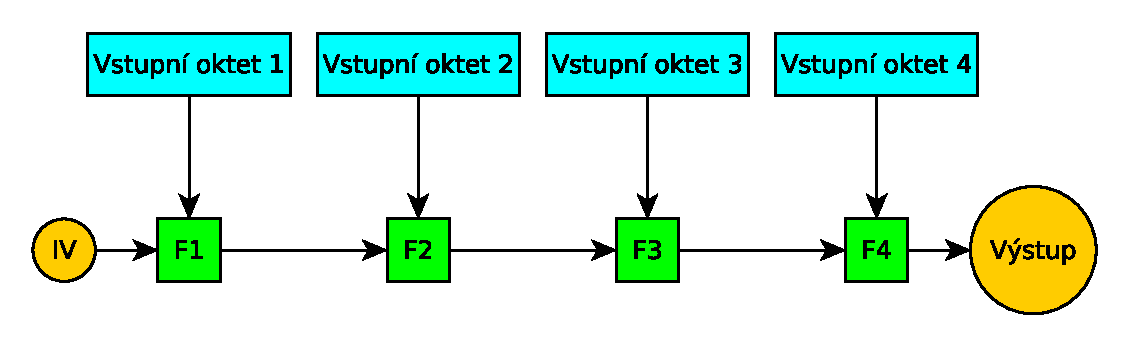
\includegraphics[width=\textwidth]{fig/merkle_damgard_design2}
	\caption{Námi upravené Merkle-Damg\r{a}rdovo schéma používá zřetězení několika různých kompresních funkcí.}
\end{figure}

Poslední změnu musí prodělat ještě množina terminálních symbolu, do které je nutné zavést příslušné symboly reprezentující
konkrétní mezivýsledky $a_0, a_1, a_2$. Ostatní parametry se oproti metodě v předchozí sekci neliší.

\section{Evoluční návrh za použití kukaččího hašování}

V poslední sérii experimentů se budeme zabývat návrhem hašovacích funkcí pro Kukaččí hašování.
Kukaččí hašování bylo popsáno v kapitole \ref{sec:hashing}, nás však bude zajímat pouze jeho
zjednodušená podoba. Provedeme stejný základní set experimentů jako v předchozích dvou případech
a vyhodnotíme výsledky.

Vzhledem k tomu, že zde pracujeme již přímo s návrhem hašovací tabulky, kdy používáme metodu pro
řešení kolizí, očekáváme výrazně lepší výsledky, než v předchozích případech. Musíme však pamatovat
na to, že naše hašovací funkce musejí být rychlé. Ačkoliv Kukaččí hašování pracuje nad všemi
operacemi v konstantním čase a to i v nejhorším případě, může být výsledná tabulka pomalá. Takový
stav může nastat v případě, že jsou jednotlivé klíče často vytlačovány (viz. funkce \Call{INSERT}{}
algoritmu \ref{alg:cuckoo_hashing}) nebo není možné vložit klíč do tabulky vůbec a je nutné
volat \Call{REHASH}{}. 

Funkci \Call{REHASH} nebudeme v našem návrhu vůbec uvažovat, protože její funkce spočívá v nalezení
nových hašovacích funkcí a znovu vytvoření hašovací tabulky. Tato operace je jedna velice časově
náročná, což by zpomalovalo výslednou hašovací tabulku a navíc bychom museli zajistit vhodné nalezení
nových hašovacích funkcí, což lze řešit například genetickým algoritmem, který však už nesmí být
součástí výsledku.

Druhým faktorem mající významný dopad na ryhlost je počet iterací vnější smyčky v operaci
\Call{INSERT}{}. S vzrůstajícím počtem iterací roste také počet volání hašovacích funkcí, které
i přes to, že jsou inherentně rychlé mohou hašovací tabulku zpomalit.

Množinu termínálních
symbolů ponecháme stejno jako v předchozích případech, stejně tak i množinu funkcí a ostatní parametry
genetického programování. Jedinou změnou bude reprezentace jedince. Ten bude tentokrát reprezentován
dvěma abstraktními syntaktickými stromy. Každý strom bude reprezentovat jednu hašovací funkci, oboum
hašovacím funkcím bude přidělena jedna polovina hašovací tabulky. Počet generací ponecháme na 100000,
neboť touto volbou fitness funkce zásadně zmenšíme prohledávací prostor.

\chapter{Experimenty s navrženými metodami}

%%%%%%%%%%%%% EXPERIMENTS WITH VARIOUS FUNCTIONS %%%%%%%%%%%%%%%
V této kapitole provedeme experimenty v nichž nejprve ověříme, zda navržené řešení poskytuje očekávané
výsledky. Poté provedeme další sérii experimentů, v níchž budeme postupně měnit parametry navrženého
řešení a vyhodnotíme výsledky. Měnit budeme jak samotné parametry algoritmu genetického
programování, tak i množiny terminálních a neterminálních symbolů. Budeme provádět vždy pouze
jednu změnu v každém experimentu, abychom zachovali jejich věrohodnost a správnou korespondenci
mezi změnou parametru a důsledkem, jaký má na výsledné řešení.

V následující sekci budeme experimentovat s evolvovanými hašovacími funkcemi, do kterých zahrneme
Merkle-Damg\r{a}rdovo schéma popsané v kapitole \ref{sec:hashing}. Krátce popíšeme změny v našem
evolučním algoritmu a provedeme příslušné experimenty.

V poslední sekci této kapitoly uvedeme do námi navrženého řešení kukaččí schéma jak bylo popsané
v kapitole \ref{sec:hashing}. Opět shrneme změny v genetickém algoritmu, provedeme a vyhodnotíme
příslušné experimenty.

Ve všech experimentech budeme měřit míru odolnosti proti kolizím, konkrétně tedy kolik je daná hašovací 
funkce schopna nahašovat různých IP adres. Další, neméně důležitou roli hraje u hašovacích funkcí jejich
rychlost. Provedeme tedy i experimenty, které odhalí rychlost s jakou jednotlivé hašovací funkce provádí svou
činnost. 

\section{Experimenty s funkcemi navrženými přímou metodou}
Nejprve se tedy budeme zkoumat výsledky, jaké poskytuje námi navržené řešení ve své přímé podobě z kapitoly
 \ref{sec:solution_design}. Námi navržený algoritmus porovnáme s náhodným prohledáváním.
 Jedná se o náhodné prohledávání s elitismem. Ta je realizována jako úprava stávajícího algoritmu tak, aby pouze mutoval.
 Mutovaným uzlem bude vždy kořen, čímž zajistíme znovuvygenerování celého kandidátního řešení.
 
 Do grafu zahrneme i jednu variantu človekem vytvořené obecné hašovací funkce, konkrétně hašovací funkci \textit{Murmurhash3} představenou
 v sekci \ref{sec:evolution_design}. Běhy námi navrženého řešení jsme promítli do grafů, kde každému
 datasetu odpovída jeden graf. Na levé straně grafu můžeme vidět průběhy námi navrženého systémů
 algoritmus náhodného prohledávání. Každá křivka je výsledkem mediánu z padesáti nezávislých běhů. Na pravé
 straně můžeme pozotovat medián systémů IPHash a u něj ještě interval spolehlivosti. Interval spolehlivosti
 je zaznačen dvěma ohraničujícímy křivkami, kde spodní značí první a horní třetí kvartil.

%%%%%%%%%%%%% IPHASH AVG Population SET #1 %%%%%%%%%%%%%%%
\begin{figure*}[!ht]
	\centering
	\begin{tikzpicture}
	\begin{axis}[ %
	, name=plot1
	, height=8cm
	, width=0.50\textwidth
	, grid=major
	, xlabel=Generation
	, ymin=5180
	, ymax=5320
	, ylabel=Successfully hashed
	, legend style=
	{ at={(1.0, 0.3)}
		, anchor=east
	}
	]
	\addplot[color=black, dashdotted, thick, mark=none] table {graph/IPHash/Set1/ElitistRandomRun_1.dat};
	\addlegendentry{Elitist Random Search}
	
	\addplot[color=green, solid, thick, mark=none] coordinates {(0,5190) (194, 5190)};
	\addlegendentry{MurmurHash3}
	
	\addplot[color=red, mark=none, dashed, thick] table {graph/IPHash/Set1/IPHashMedian_1.dat}; 
	\addlegendentry{Proposed IPHash}
	
	\end{axis}
	
	\begin{axis}[ %
	, name=plot2
	, at=(plot1.right of south east)
	, anchor=left of south west
	, ymin=5180
	, ymax=5320
	, height=8cm
	, width=0.50\textwidth
	, grid=major
	, xlabel=Generation
	%%	, ylabel=Successfully hashed
	, yticklabels={,,}
	%%	, legend pos=outer north east
	, legend style=
	{ at={(1.0, 0.3)}
		, anchor=east
	}
	]
	\addplot[color=red, mark=none, dashed,thick] table {graph/IPHash/Set1/IPHashMedian_1.dat}; 
	\addlegendentry{Proposed IPHash}
	\addplot[color=red, mark=none, dotted] table {graph/IPHash/Set1/IPHashReliab1_1.dat}; 
	%\addlegendentry{Proposed IPHash RR1}
	\addplot[color=red, mark=none, dotted] table {graph/IPHash/Set1/IPHashReliab3_1.dat}; 
	\addlegendentry{Diversity of runs}
	\end{axis}
	\end{tikzpicture}
	\caption{Evolvované hašovací funkce a jejich fitnes hodnota nad data setem číslo 1. TODO: FIX THIS}
	\label{fig:basicComparison1}
\end{figure*}
%%%%%%%%%%%%% IPHASH AVG Population SET #1 %%%%%%%%%%%%%%%

Na obrázku \ref{fig:basicComparison1} můžeme vidět vidět porovnání běhů a jejich výsledků obou algoritmů.
Je patrné, že nad prvním datasetem, navržené řešení jasně dominuje nad náhodným prohledáváním. IPHash
nahašoval o 25 IP adres více než druhý nejůspěšnější algoritmus náhodného prohledávání. Nejhůře si vedl
člověkem vytvořený algoritmus \textit{MurmurHash3}, který nahašoval o celých 111 IP adres méně. 

Z intervalu spolehlivost můžeme usoudit, že námi navržený algoritmus skutečně dobře a rozptyly jeho
řešení nejsou příliš signifikantní, ale je zde prostor pro zlepšení . Nalezené řešení není tedy dílem čísté náhody. Z grafu můžeme vyčíst, že 
algoritmus v prních několika generacích rapidně konverguje a s postupným příbýváním generací se jeho 
konvergence zpomaluje. Jedná se o téměř ukázkový běh algoritmu genetického programování \cite{GPTutorial}.

%%%%%%%%%%%%% IPHASH AVG Population SET #2 %%%%%%%%%%%%%%%
\begin{figure*}[!ht]
	\centering
	\begin{tikzpicture}
	\begin{axis}[ %
	, name=plot1
	, height=8cm
	, width=0.50\textwidth
	, grid=major
	, xlabel=Generation
	, ymin=5180
	, ymax=5330
	, ylabel=Successfully hashed
	, legend style=
	{ at={(1.0, 0.3)}
		, anchor=east
	}
	]
	\addplot[color=black, dashdotted, thick, mark=none] table {graph/IPHash/Set2/ElitistRandomRun_2.dat};
	\addlegendentry{Elitist Random Search}
	
	\addplot[color=green, solid, thick, mark=none] coordinates {(0,5190) (194, 5190)};
	\addlegendentry{MurmurHash3}
	
	\addplot[color=red, mark=none, dashed, thick] table {graph/IPHash/Set2/IPHashMedian_2.dat}; 
	\addlegendentry{Proposed IPHash}
	
	\end{axis}
	
	\begin{axis}[ %
	, name=plot2
	, at=(plot1.right of south east)
	, anchor=left of south west
	, ymin=5180
	, ymax=5330
	, height=8cm
	, width=0.50\textwidth
	, grid=major
	, xlabel=Generation
	%%	, ylabel=Successfully hashed
	, yticklabels={,,}
	%%	, legend pos=outer north east
	, legend style=
	{ at={(1.0, 0.3)}
		, anchor=east
	}
	]
	\addplot[color=red, mark=none, dashed,thick] table {graph/IPHash/Set2/IPHashMedian_2.dat}; 
	\addlegendentry{Proposed IPHash}
	\addplot[color=red, mark=none, dotted] table {graph/IPHash/Set2/IPHash1stQ_2.dat}; 
	%\addlegendentry{Proposed IPHash RR1}
	\addplot[color=red, mark=none, dotted] table {graph/IPHash/Set2/IPHash3rdQ_2.dat}; 
	\addlegendentry{Diversity of runs}
	\end{axis}
	\end{tikzpicture}
	\caption{Evolvované hašovací funkce a jejich fitnes hodnota nad data setem číslo 2.}
	\label{fig:basicComparison2}
\end{figure*}
%%%%%%%%%%%%% IPHASH AVG Population SET #2 %%%%%%%%%%%%%%%

V případě druhého datasetu jsou dosažené výsledky (\ref{fig:basicComparison2}) ještě lepší. IPHash dosáhl vyššího mediánu
a opět výrazně převýšil jak náhodné prohledávání, tak \textit{MurmurHash3}. Nahašoval o 24
IP adres více než náhodné prohledávání a o 115 IP adres více, než \textit{MurmurHash3}. 
Interval spolehlivosti je s výjimkou posledních několika generací více sevřený kolem křivky
IPHash, což značí spolehlivý algoritmus. Stejně jako v předchozím případě, algoritmus rapidně
konverguje v prvních několika generacích. Poté jeho nástup ustává.

%%%%%%%%%%%%% IPHASH AVG Population SET #3 %%%%%%%%%%%%%%%
\begin{figure*}[!ht]
	\centering
	\begin{tikzpicture}
	\begin{axis}[ %
	, name=plot1
	, height=8cm
	, width=0.50\textwidth
	, grid=major
	, xlabel=Generation
	, ymin=5180
	, ymax=5320
	, ylabel=Successfully hashed
	, legend style=
	{ at={(1.0, 0.3)}
		, anchor=east
	}
	]
	\addplot[color=black, dashdotted, thick, mark=none] table {graph/IPHash/Set3/ElitistRandomRun_3.dat};
	\addlegendentry{Elitist Random Search}
	
	\addplot[color=green, solid, thick, mark=none] coordinates {(0,5206) (194, 5206)};
	\addlegendentry{MurmurHash3}
	
	\addplot[color=red, mark=none, dashed, thick] table {graph/IPHash/Set3/IPHashMedian_3.dat}; 
	\addlegendentry{Proposed IPHash}
	
	\end{axis}
	
	\begin{axis}[ %
	, name=plot2
	, at=(plot1.right of south east)
	, anchor=left of south west
	, ymin=5180
	, ymax=5320
	, height=8cm
	, width=0.50\textwidth
	, grid=major
	, xlabel=Generation
	%%	, ylabel=Successfully hashed
	, yticklabels={,,}
	%%	, legend pos=outer north east
	, legend style=
	{ at={(1.0, 0.3)}
		, anchor=east
	}
	]
	\addplot[color=red, mark=none, dashed,thick] table {graph/IPHash/Set3/IPHashMedian_3.dat}; 
	\addlegendentry{Proposed IPHash}
	\addplot[color=red, mark=none, dotted] table {graph/IPHash/Set3/IPHash1stQ_3.dat}; 
	%\addlegendentry{Proposed IPHash RR1}
	\addplot[color=red, mark=none, dotted] table {graph/IPHash/Set3/IPHash3rdQ_3.dat}; 
	\addlegendentry{Diversity of runs}
	\end{axis}
	\end{tikzpicture}
	\caption{Evolvované hašovací funkce a jejich fitnes hodnota nad data setem číslo 3.}
	\label{fig:basicComparison3}
\end{figure*}
%%%%%%%%%%%%% IPHASH AVG Population SET #3 %%%%%%%%%%%%%%%

Zajímavá situace nastala v případě třetího datasetu \ref{fig:basicComparison3}. Na první pohled je patrné,
že oba iterační algoritmy zde řešení s obdobnou hodnotou fitnes. Dále je vidět,
že mediánová hodnota fitnes se nám znatelně a to o více než dvacet nahašovaných 
adres v případě algoritmu IPHash. Výsledná řešení náhodného prohledávání našla
řešení s obdobnou hodnotou fitnes jako v předchozím případě. Naopak se zvýšila 
hodnota u algoritmu \textit{MurmurHash3}, a to o celýh 15 nahašovaných adres.

Z intervalu spolehlivosti můžeme vyčíst, mnohem větší rozptyl než v předchozích
případech. IPHash algoritmus produkuje mnohem větší diverzitu v nalezených řešeních.
Tento fakt ve spojení s obdobnou hodnotou fitnes funkce jako má náhodné prohledávání
značí, že stavový prostor tak jak modelován třetím datasetem je vhodný spíše pro 
algoritmus náhodného prohledávání, než pro evoluční algoritmus. Evoluční algoritmus
se v prostoru dostupných řešení ``nemá čeho chytit''. Proto špatně konverguje a jeho
průběh připomíná náhodné prohledávání. Na počátku algoritmus konverguje velmi rychle
velmi rychle však ztrácí veškerý progres a téměř úplně staguje.

%%%%%%%%%%%%% IPHASH AVG Population SET #4 %%%%%%%%%%%%%%%
\begin{figure*}[!ht]
	\centering
	\begin{tikzpicture}
	\begin{axis}[ %
	, name=plot1
	, height=8cm
	, width=0.50\textwidth
	, grid=major
	, xlabel=Generation
	, ymin=5180
	, ymax=5320
	, ylabel=Successfully hashed
	, legend style=
	{ at={(1.0, 0.3)}
		, anchor=east
	}
	]
	\addplot[color=black, dashdotted, thick, mark=none] table {graph/IPHash/Set4/ElitistRandomSearch_4.dat};
	\addlegendentry{Elitist Random Search}
	
	\addplot[color=green, solid, thick, mark=none] coordinates {(0,5206) (194, 5206)};
	\addlegendentry{MurmurHash3}
	
	\addplot[color=red, mark=none, dashed, thick] table {graph/IPHash/Set4/IPHashMedian_4.dat}; 
	\addlegendentry{Proposed IPHash}
	
	\end{axis}
	
	\begin{axis}[ %
	, name=plot2
	, at=(plot1.right of south east)
	, anchor=left of south west
	, ymin=5180
	, ymax=5320
	, height=8cm
	, width=0.50\textwidth
	, grid=major
	, xlabel=Generation
	%%	, ylabel=Successfully hashed
	, yticklabels={,,}
	%%	, legend pos=outer north east
	, legend style=
	{ at={(1.0, 0.3)}
		, anchor=east
	}
	]
	\addplot[color=red, mark=none, dashed,thick] table {graph/IPHash/Set4/IPHashMedian_4.dat}; 
	\addlegendentry{Proposed IPHash}
	\addplot[color=red, mark=none, dotted] table {graph/IPHash/Set4/IPHash1stQ_4.dat}; 
	%\addlegendentry{Proposed IPHash RR1}
	\addplot[color=red, mark=none, dotted] table {graph/IPHash/Set4/IPHash3rdQ_4.dat}; 
	\addlegendentry{Diversity of runs}
	\end{axis}
	\end{tikzpicture}
	\caption{Evolvované hašovací funkce a jejich fitnes hodnota nad data setem číslo 4.}
	\label{fig:basicComparison4}
\end{figure*}
%%%%%%%%%%%%% IPHASH AVG Population SET #4 %%%%%%%%%%%%%%%

Zdá se, že stejně jako v předchozím případě, se IPHash chová i nad posledním datasetem čtyři (\ref{fig:basicComparison4}).
Mediánová hodnota je opět nižší než v případě náhodného prohledávání. Je však vyšší, než v případě
\textit{MurmurHash3}. Stavový prostor, zda se, má opět náhodnou charakteristiku a algoritmus spatně
koverguje. Rozptyl je opět větší než v prvních dvou případech. Algoritmus rychle konverguje v prvních
několika generacích. Brzy však přejde ve stagnaci.

Dříve, než se pustíme dále je vhodné se zamyslet na doposud dosaženými výsledky algoritmem náhodného
prohledávání. Teoreticky algoritmus náhodného prohledávání je takový, který náhodně vybírá body
daného stavového prostoru. Součástí každého evolučního algoritmu je však také reprezentace problému,
která modeluje stavový prostor. V našem případě bylo náhodné proheldávání velmi silně ovlivněno 
reprezentací jednců jako abstraktních syntaktických stromů a použitými terminálními a funkčními symboly.
Lze tedy stále mluvit o algoritmu náhodného prohledávání, mějme však na paměti, že výsledky jím
dosaženou jsou velkou měrou způsobené právě námi vhodně zvolenou reprezentací.

Jedna ze zajímavých vlastostí společnou pro všechny grafy je fakt, že v iniciálních populacích obou
iteračních algoritmů jsme nalezli řešení, která převyšovala člověkem vytvořené hašovací funkce. Toto
je velmi zajímavý poznatek. Důvodem je, že velikost populace jsme zvolili poměrně velkou. I přes to
však z toho plyne, že po několika málo pokusech s náhodným generováním abstraktních syntaktických 
stromů můžeme nalézt řešení, která převyšují ta člověkem vytvořená.

\begin{table}[!ht]
	\centering
	\begin{tabular}{l|c|c|c|c}
		Hašovací funkce & Dataset 1 & Dataset 2 & Dataset 3 & Dataset 4 \\
		\hline
		FarmHash             & 5227 & 5199 & 5203 & 5158 \\
		MurmurHash3    		 & 5190 & 5190 & 5206 & 5206 \\
		CityHash             & 5180 & 5156 & 5171 & 5155 \\
		\hline
		IPHash               & 5301 & 5305 & 5274 & 5278 \\
		Náhodné prohledávání & 5276 & 5281 & 5277 & 5281 \\
		\hline
	\end{tabular}
	\caption{Shrnutí výsledků evolvovaných i obecných hašovacích funkcí napříč všemi datasety.}
	\label{tab:IPHash_conclusion}
\end{table}

Ve shrnující tabulkce \ref{tab:IPHash_conclusion} můzeme vidět výsledky algoritmu náhodného prohledávání
a algoritmu IPHash v kontrastu s člověkem vytvořenými hašovacími funkcemi z kapitoly \ref{sec:hashing}.
Nad prvními dvěma má nejlepší mediánovou hodnotu fitnes IPHash. Nad druhými dvěma naopak náhodné prohledávání.
Člověkem vytvořené algoritmy ani v jednom případě napřekonaly IPHash. Naopak IPHash nad obecnými hašovacími
funkcemi jasně dominuje. Rozdíl je nejvíce znát v v případě funkce \textit{CityHash} nad datasetem dva, kde se rozdíl
rovná hodnotě 150 nahašovaných funkcí. Nejméně je to naopak v případě funkce \textit{FarmHash} nad datasetem tři,
kde se rozdíl zmenšil na 71 nahašovaných adres.
 
Nyní se budeme podrobněji zabývat rozptylem nejlepšího nalezeného řešení (ekvivalent
hodnoty poslední generace algoritmu), které  nalezne náhodné prohledávání a IPHash v porovnání s
algoritmem náhodného prohledávání.

%%%%%%%%%%%%% IPHASH BOXPLOT %%%%%%%%%%%%%%%
\begin{figure}[!h]
	\centering
	\begin{tikzpicture}
	\begin{axis}
	[ boxplot/draw direction=y
	, name=plot1
	, xtick={1,2,3}
	, xticklabels={RS, IPHash, Náhodné prohledávání}
	, ymin=5200
	, ymax=5360
	]
	\addplot+[
	boxplot prepared={
		lower whisker=5250,
		lower quartile=5266,
		median=5276,
		upper quartile=5286,
		upper whisker=5311,
	},
	] coordinates {}; % RS
	
	\addplot+[
	boxplot prepared={
		lower whisker=5279,
		lower quartile=5292,
		median=5301,
		upper quartile=5315,
		upper whisker=5352,
	},
	] coordinates {}; % IPHash
	
	\addplot+[
	boxplot prepared={
		lower whisker=5242,
		lower quartile=5265,
		median=5274,
		upper quartile=5286,
		upper whisker=5319,
	},
	] coordinates {}; % ERS
	\end{axis}		

	\begin{axis}
	[ boxplot/draw direction=y
	, name=plot2
	, at=(plot1.right of south east)
	, xtick={1,2,3}
	, xticklabels={RS, IPHash, Náhodné prohledávání}
	, ymin=5200
	, ymax=5360
	, yticklabels={,,}
	]		
	\addplot+[color=blue,
		boxplot prepared={
		lower whisker=5255,
		lower quartile=5270,
		median=5281,
		upper quartile=5290,
		upper whisker=5331,
	},
	] coordinates {}; % RS
	
	\addplot+[color=red,
		boxplot prepared={
			lower whisker=5286,
			lower quartile=5298,
			median=5305,
			upper quartile=5319,
			upper whisker=5352,
		},
		] coordinates {}; % IPHash
		
	\addplot+[
	boxplot prepared={
		lower whisker=5251,
		lower quartile=5270,
		median=5279,
		upper quartile=5285,
		upper whisker=5328,
	},
	] coordinates {}; % ERS
	\end{axis}		
	\end{tikzpicture}
	\caption{Porovnání výsledků algirutmu IPHash a náhodného porovnání krabicovým diagramem pro datasety jedna a dvě.}
	\label{fig:basic_boxplot_1}
\end{figure}

Na dvou krabicových diagramech grafech na obrázku \ref{fig:basic_boxplot_1}, vidíme porovnání
algoritmů v nad datasety jedna dvě. Nad těmito datasety si algoritmus vedl velmi dobře, a to potvrzují
i krabicové diagramy. V celém rozsahu rozptylu námi navrženého řešení dostáváme lepší výsledky, než u
algoritmu náhodného prohledávání a to v obou případech. Nejlepší řešení nalezené algoritmem náhodného
prohledávání je jen nepatrně výše, než horní hranice rozptylu algoritmu IPHash. Nejhorší řešení nalezené
algoritmem IPHash je v případě prvního datasetu lepší než medián algoritmu náhodného prohledávání a
v případě druhého datasetu dokonce lepší, než nejlepší řešení rozptylu náhodného prohledávání. Co se týče
nejlepšího řešení algoritmu IPHash, tak to značně převušuje i to nejlepší řešení nalezené algoritmem
náhodného prohledávání. Je tedy patrné, že ve všech případech algoritmus IPHash dobře konvergoval v daném
stavovém prostoru popsaném fitnes funkcí a zvolenou reprezentací jedinců.

\begin{figure}[!h]
\centering
\begin{tikzpicture}
	\begin{axis}
	[ boxplot/draw direction=y
	, name=plot3	
	, xtick={1,2,3}
	, xticklabels={RS, IPHash, Náhodné prohledávání}
	, ymin=5200
	, ymax=5360
	]		
	\addplot+[
	boxplot prepared={
		lower whisker=5246,
		lower quartile=5268,
		median=5277,
		upper quartile=5290,
		upper whisker=5302,
	},
	] coordinates {}; % RS
	
	\addplot+[
	boxplot prepared={
		lower whisker=5242,
		lower quartile=5261,
		median=5274,
		upper quartile=5287,
		upper whisker=5342,
	},
	] coordinates {}; % IPHash
	
	\addplot+[
	boxplot prepared={
		lower whisker=5237,
		lower quartile=5263,
		median=5275,
		upper quartile=5289,
		upper whisker=5318,
	},
	] coordinates {}; % ERS
	\end{axis}		

	\begin{axis}
	[ boxplot/draw direction=y
	, name=plot4
	, at=(plot3.right of south east)
	, xtick={1,2,3}
	, xticklabels={RS, IPHash, Náhodné prohledávání}
	, yticklabels={,,}
	, ymin=5200
	, ymax=5360
	]		
	\addplot+[
	boxplot prepared={
		lower whisker=5251,
		lower quartile=5269,
		median=5281,
		upper quartile=5285,
		upper whisker=5310,
	},
	] coordinates {}; % RS
	
	\addplot+[
	boxplot prepared={
		lower whisker=5252,
		lower quartile=5264,
		median=5278,
		upper quartile=5285,
		upper whisker=5298,
	},
	] coordinates {}; % IPHash
	
	\addplot+[
	boxplot prepared={
		lower whisker=5251,
		lower quartile=5268,
		median=5276,
		upper quartile=5290,
		upper whisker=5323,
	},
	] coordinates {}; % ERS
	\end{axis}		

	\end{tikzpicture}
	\caption{Porovnání výsledků algirutmu IPHash a náhodného porovnání krabicovým diagramem pro datasety tři a čtyři.}
	\label{fig:basic_boxplot_2}
\end{figure}
%%%%%%%%%%%%% IPHASH BOXPLOT %%%%%%%%%%%%%%%

V kontrastu s výsledky nad prvními dvěma datasety jsou výsledky nad druhými dvěma datasety. V obou případech
si námi navržené řešení nevedlo v průměru lépe, než algorimus náhodného prohledávání. Je vidět, že nejlepší
nalezená řešení mají obdobný rozptyl. Nad datasetem číslo tři je rozptyl velmi podobný, těsně ve prospěch 
náhodného prohledávání. Medián lze považovat za totožný. Nejlepší nalezené řešení však jasně mluví ve prospěch
algoritmu IPHash, kde je rozdíl více než dvacet úspěšně nahašovaných adres. V případě datasetu číslo ctyři náhodné
prohledávání jasně předčilo námi navržený algoritmus. I přes to, že je mediánová hodnota náhodného prohledávání
nepatrně menší, je zanedbatelná a lze ji považovat za nepřesnost měření. Horní i spodní hranice rozptylu náhodného
prohledávání je položena výše než v případě algoritmu IPHash. Celkem lze pozorovat, že ani jeden algoritmus 
nenašel řešení, které by mohlo konkurovat nejlepším výslekům dosaženým v nad předešlými datasety. I přes to
nejlepší nalezené řešení jednoznačně mluví ve prospěch algoritmu náhodného prohledávání.

Nejlepších výsledků bylo dosaženo nad prvními dvěma datasety, kde v obou případech si nejlépe vedl námi navržený
algoritmus. U třetího datasetu se výsledky zhoršili v porovnání s předchozími a to u obou algoritmů. Oba si byly 
rovnocéné, ale nejlepší řešení nalezl algoritmus IPHash. V případě posledního datasetu jsou výsledky podobné jako
v případě datasetu tři. Nejlepší řešení nalezlo náhodné prohledávání, ale i zde můžeme pozorovat zhořšení. 

Správná volba hloubky abstraktního stromu kandidátního řešení má zásadní vliv jak na kvalitu vyevolvovaných řešení,
tak i na rychlost. Předpokládáme, že větší hloubka stromu implikuje větší prohledávací prostor algoritmu, v kterém
se vyskytují i kvalitní řešení. Musíme však brát v potaz to, že velmi hluboké stromy reprezentují složitá a velká kandidátní
řešení, která mohou neúměrně zpomalovat výpočet hašovací funkce. Důležitým aspektem genetického programování je 
dobrá volba velikosti počáteční generace. Ta se typicky používá co nejvyšší (až tisíce jedinců), aby algoritmus nalezl
optimální řešení v prvních padesátí generacích \cite{GPTutorial}.

V následující části tedy prozkoumáme, jaký vliv má na hodnotu fitnes volba maximální hloubky abstraktního syntaktického
stromu kandidátních řešení v závislosti na velikosti populace. To nám zároveň umožní si ověřit, zda jsme tyto parametry
zvolili správně v návrhu řešení \ref{sec:solution_design}.

%%%%%%%%%%%%% IPHASH Population depth %%%%%%%%%%%%%%%
\begin{figure}[!ht]
\centering
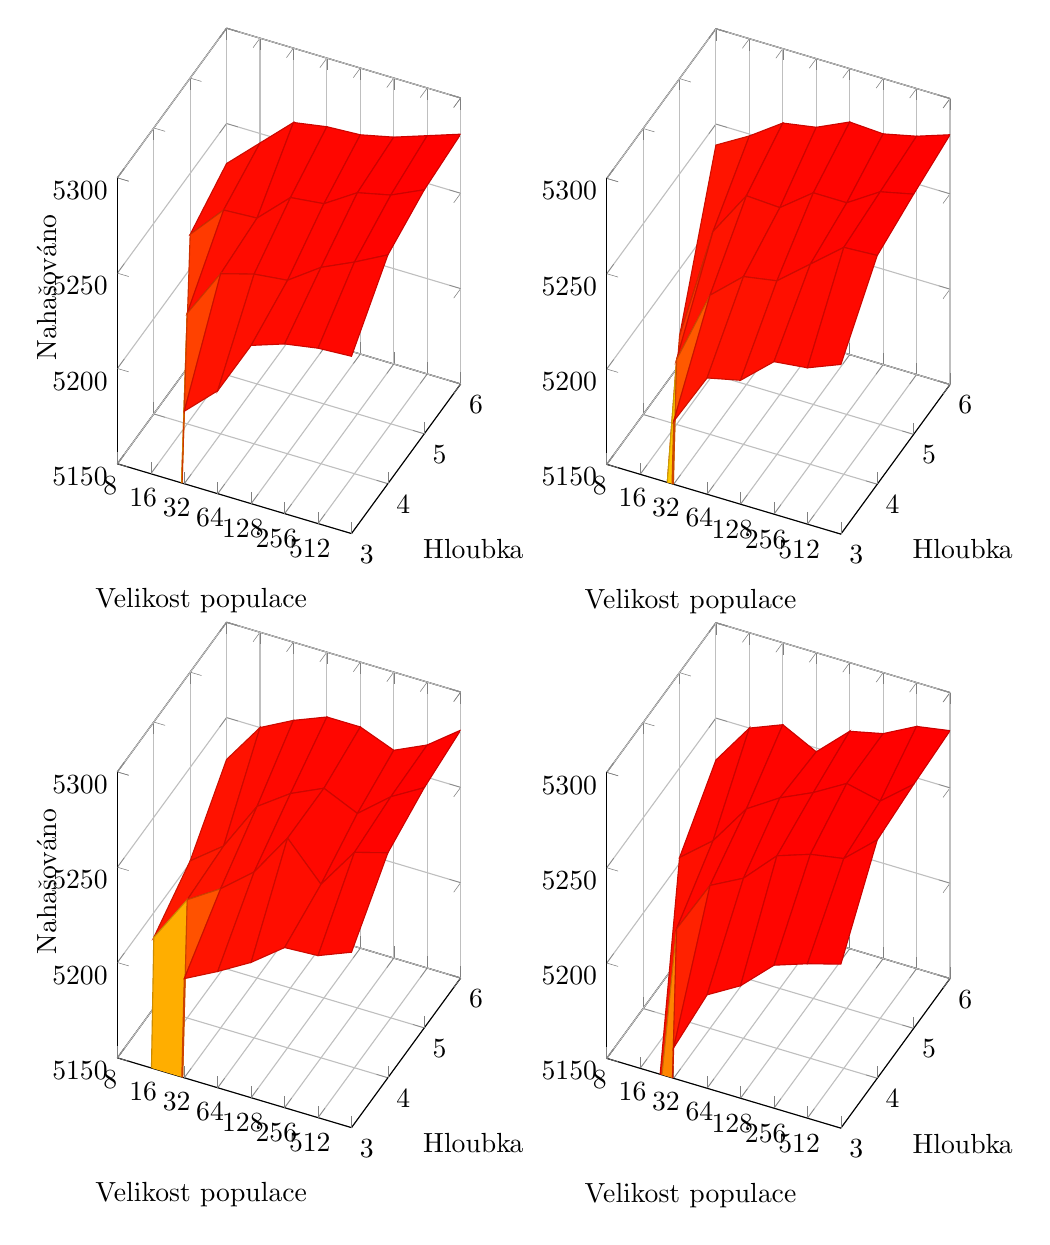
\begin{tikzpicture}
	\begin{axis}[ 
	, grid=major
	, name=plot1
	, width=0.49\linewidth
	, height=8cm
	, legend pos=outer north east
	, xlabel={Velikost populace}
	, xtick={1,2,3,4,5,6,7,8}
	, xticklabels={8,16,32,64,128,256,512}
	, ylabel={Hloubka}
	, ytick={3,4,5,6}
	, zlabel style={ at={(-0.15,0.5)}} 
	, zlabel={Nahašováno}
	, zmin=5150 %{5280,5290,5300,5310,5320}
	, zmax=5300 %
	, ztick={5150,5200,5250,5300}
	, zticklabels={5150,5200,5250,5300}
	]
	\addplot3[surf] coordinates {
		    %8            16         32          64         128        256        512       1024  
		    (1,3,4000) (2,3,4603) (3,3,5188) (4,3,5204) (5,3,5233) (6,3,5239) (7,3,5242) (8,3,5243)
		    
		    (1,4,4680) (2,4,5208) (3,4,5234) (4,4,5239) (5,4,5241) (6,4,5253) (7,4,5261) (8,4,5270)
		    
		    (1,5,5218) (2,5,5236) (3,5,5237) (4,5,5253) (5,5,5255) (6,5,5266) (7,5,5270) (8,5,5278)
		    
		    (1,6,5229) (2,6,5245) (3,6,5261) (4,6,5264) (5,6,5265) (6,6,5269) (7,6,5275) (8,6,5281) 
		};
	\end{axis}
	
	\begin{axis}[ 
	, grid=major
	, name=plot2
	, width=0.49\linewidth
	, height=8cm
	, anchor=outer north west
	, at=(plot1.right of north east)
	, legend pos=outer north east
	, xlabel={Velikost populace}
	, xtick={1,2,3,4,5,6,7,8}
	, xticklabels={8,16,32,64,128,256,512}
	, ylabel={Hloubka}
	, ytick={3,4,5,6}
	, zlabel style={ at={(-0.15,0.5)}} 
%	, zlabel={Nahašováno}
	, zmin=5150 %{5280,5290,5300,5310,5320}
	, zmax=5300 %
	, ztick={5150,5200,5250,5300}
	, zticklabels={5150,5200,5250,5300}
	]
	\addplot3[surf] coordinates {
		%8            16              32              64             128            256           512           1024  
		(1,3,4158) (2,3,4481) (3,3,5183) (4,3,5211) (5,3,5215) (6,3,5230) (7,3,5232) (8,3,5239)
		
		(1,4,4947) (2,4,5184) (3,4,5223) (4,4,5238) (5,4,5241) (6,4,5255) (7,4,5269) (8,4,5270)
		
		(1,5,5165) (2,5,5225) (3,5,5249) (4,5,5248) (5,5,5261) (6,5,5261) (7,5,5272) (8,5,5276)
		
		(1,6,5239) (2,6,5249) (3,6,5261) (4,6,5264) (5,6,5272) (6,6,5271) (7,6,5275) (8,6,5281) 
	};
	\end{axis}

	\begin{axis}[ 
	, grid=major
	, name=plot3
	, width=0.49\linewidth
	, height=8cm
	, anchor=north west
	, at=(plot1.below south west)
	, legend pos=outer north east
	, xlabel={Velikost populace}
	, xtick={1,2,3,4,5,6,7,8}
	, xticklabels={8,16,32,64,128,256,512}
	, ylabel={Hloubka}
	, ytick={3,4,5,6} 
	, zlabel style={ at={(-0.15,0.5)}}
	, zlabel={Nahašováno}
	, zmin=5150 %{5280,5290,5300,5310,5320}
	, zmax=5300 %
	, ztick={5150,5200,5250,5300}
	, zticklabels={5150,5200,5250,5300}
	]
	\addplot3[surf] coordinates {
		%8            16         32          64         128        256        512       1024  
		(1,3,4137) (2,3,4498) (3,3,5202) (4,3,5211) (5,3,5221) (6,3,5234) (7,3,5235) (8,3,5242)
		
		(1,4,5187) (2,4,5212) (3,4,5223) (4,4,5237) (5,4,5260) (6,4,5241) (7,4,5263) (8,4,5268) % 5,4 coordinate didnt complete FIX IT
		
		(1,5,5201) (2,5,5214) (3,5,5240) (4,5,5252) (5,5,5260) (6,5,5252) (7,5,5266) (8,5,5276)
		
		(1,6,5228) (2,6,5250) (3,6,5259) (4,6,5266) (5,6,5266) (6,6,5259) (7,6,5267) (8,6,5280) 
	};
	\end{axis}
	
	\begin{axis}[ 
	, grid=major
	, name=plot4
	, width=0.49\linewidth
	, height=8cm
	, anchor=outer north west
	, at=(plot3.right of north east)
	, legend pos=outer north east
	, xlabel={Velikost populace}
	, xtick={1,2,3,4,5,6,7,8}
	, xticklabels={8,16,32,64,128,256,512}
	, ylabel={Hloubka}
	, ytick={3,4,5,6} 
	, zlabel style={ at={(-0.15,0.5)}}
%	, zlabel={Nahašováno}
	, zmin=5150 %{5280,5290,5300,5310,5320}
	, zmax=5300 %
	, ztick={5150,5200,5250,5300}
	, zticklabels={5150,5200,5250,5300}
	]
	\addplot3[surf] coordinates {
		%8            16         32          64         128        256        512       1024  
		(1,3,2499) (2,3,4533) (3,3,5166) (4,3,5199) (5,3,5209) (6,3,5225) (7,3,5231) (8,3,5236)
		
		(1,4,5016) (2,4,5197) (3,4,5225) (4,4,5234) (5,4,5251) (6,4,5257) (7,4,5260) (8,4,5275) 
				
		(1,5,5203) (2,5,5217) (3,5,5239) (4,5,5250) (5,5,5258) (6,5,5268) (7,5,5264) (8,5,5278)
		
		(1,6,5228) (2,6,5250) (3,6,5257) (4,6,5248) (5,6,5264) (6,6,5268) (7,6,5277) (8,6,5280) 
	};
	\end{axis}
\end{tikzpicture}
\caption{Počet úspěšně nahašovaných IP adres v závislosti na velikosti populace a maximální hloubce kandidátního řešení. 
	Uvedeny jsou výsledky naříč datasety jedna (vlevo nahoře), dvě (vpravo nahoře), tři (vlevo dole) a čtyři (vpravo dole).}
\label{fig:basicPopulationDepth1}
\end{figure}

Výsledky vidíme zobrazené jako tří rozměrné grafy na obrázku \ref{fig:basicPopulationDepth1}. Na všech čtyřech grafech
zobrazující výsledky nad jednotlivými datasety je patrné, že pro velmi malé populace (8 a 16 jedinců) nenalezne agoritmus
IPHash dobré hašovací funkce. Jejich hodnota fitnes je o několik tisíc nahašovaných adres menší (nelze rozumně zobrazit na grafu).
Pro exponenciálně vzrůstající velikost velikost populace roste však hodnota fitnes jen střídmě. Je vidět, že neustálým zvětšováním
velikosti populace lepších výsledků nedosáhneme, i přes to že se velikost populace o hodnotě 1024 jedinců jeví jako lepší volba.

Obdobně je tomu při zvyšování hloubky stromu. Zde je přírůstek lineární (nikoli exponenciální jako v případě populace). I zde můžeme
pozorovat předpokládanou tendenci algoritmu IPHash zvyšovat hodnotu fitnes s přibývající maximální hloubkou stromu a tedy se 
zvětšujícím se prohledávaným prostorem. Zajímavý je fakt, že s přibývající velikostí populace se zvětšuje i hodnota fitnes u mělkých
abstraktních syntaktických stromů (hloubky 3 a 4). Velké populace tedy dokážou nalézt kvalitní řešení i v relativně mělkých stromech.
Toto je zásadní poznatek, který nám umožní v případě potřeby rozumně přesunout důraz na rychlost volbou mělčích stromů, aniž by
zásadně (jedná se přibližně o rozdíl 50 nahašovaných adres) utrpěla hodnota fitnes. Dále můžeme pozorovat některé zajímavé vlastnosti. 

\begin{itemize}
	\item První z nich je četnost výstupků na ploše grafu. V případě prvních dvou datasetů jsou plochy grafů relativně ``hladké''. Naproti tomu v
		případě datasetů tři a čtyři, můžeme pozorovat několik propadlých nebo vystouplých bodů. To může svědčit o deformovaném
		prohledávaném prostoru kandidátních řešení, jak jsme mohli vidět i v předchozí části této sekce. Může se však jednat i o náhodu.
		
	\item Hlubší abstraktní syntaktické stromy se zdají být méně náchylné na zvolenou velikost populace. Na všech čtyřech datasetech již
		od velikosti populace 32 jedinců můžeme pozorovat dobré výsledky. Můžeme tedy tvrdit, že volba velikosti populace ovlivňuje zejména
		mělké abstraktní syntaktické stromy. 
\end{itemize}

%%%%%%%%%%%%% IPHASH Population depth %%%%%%%%%%%%%%%

Zkusme si nyní ověřit naši volbu volbu funkčních a terminálních symbolů. To můžeme provést přídáním, či odebraním 
pouze jednoho neterminálu v každém kroku a sledováním výsledků kvality navržených hašovacích funkcí. Přídáním či
odebráním více než jednoho terminálu v jednom kroku, bychom nebyly schopni interpretovat dosažené výsledky. V 
následující sérii experimentů budeme s očekávaným úbytkem hodnoty fitness odebírat funkční a terminální symboly.
Při přídání některého funkčního nebo terminálního symbolu budeme naopak očekávat kýžený nárůst hodnoty fitnes 
signalizující lepší řešení Výsledky experimentů můžeme vidět v tabulce \ref{tab:basicRunAlternatives1}.

\begin{table}[h]
	\centering
	\caption{Vliv různých voleb and terminálních a neterminálních množin na výslednou hodnotu fitnes. Experimenty jsou provedeny
		napříč všemi datasety.}
	\begin{tabular}{lcccccc} \\ \hline
		   & & & \multicolumn{4}{c}{Dataset} \\
		   & Terminální množína & Funkční množina & 1 & 2 & 3 & 4 \\ \hline
		1. & $\{o_{0} .. o_{3}, \Re \}$ & $\{*, +, \wedge, \ggg\}$         & 5307 & 5305     & 5274 & 5278 \\
		2. & $\{o_{0} .. o_{3}\}$ & $\{*, +, \wedge, \ggg\}$                  & 5291 & 5269    & 5273 & 5270  \\
		3. & $\{o_{0} .. o_{3}, \Re \}$ & $\{*, +, \wedge, \neg, \ggg\}$ & 5300 & 5274.5 & 5271 &  5269.5 \\
		4. & $\{o_{0} .. o_{3}, \Re \}$ & $\{*, \wedge, \ggg\}$              & 5306 & 5274.5 & 5270 & 5276 \\
		5. & $\{o_{0} .. o_{3}, \Re \}$ & $\{+, \wedge, \ggg\}$ 			   & 5290 & 5270    & 5269  & 5268 \\
		6. & $\{o_{0} .. o_{3}, \Re \}$ & $\{*, +, \wedge\}$                   & 5298 & 5269    & 5272 & 5270 \\
		7. & $\{o_{0} .. o_{3}, \Re \}$ & $\{+, \wedge\}$                      & 5065 & 4962     & 5018 & 4992 \\
		\hline
	\end{tabular}
	\label{tab:basicRunAlternatives1}
\end{table}

Na prvním řádku tabulky můžeme vidět mediánový průměr hodnoty fitness z 50 nezávislých běhů. Toto původní
navržené řešení a budeme jej pro tuto chvíli považovat za referenční a budeme zkoumat, zda bychom jinou
volbou terminální a neterminální množiny nedosáhli lepších výsledků. 

Nejprve z množiny terminálů odebereme náhodnou konstantu $\Re$ reprezentovanou prvočíslem (řádek 2. v tabulce
\ref{tab:basicRunAlternatives1}).
Většina state-of-the-art
hašovacích funkcí si pomáhá právě nějakou formou náhodné konstanty pro zlepšení svých výstupů, její odebrání by tedy
mělo mít negativní vliv na hodnotu fitness. Na prvních dvou
datasetech je vidět znatelný pokles v hodnotě fitness a to o 16 adres v prvním případě a o celých 36 adres
v případě druhém. Na datasetech tři a čtyři je však pokles méně patrný a dal by se považovat za nevýznamný.

Nepříliš často viděným operátorem ve obecných hašovacích funkcích je operátor jedničkového doplňku ($\neg$).
Tento operátor
spolu s operátorem XOR tvoří uplnou bázi logických spojek a jsou tedy schopné vytvořit libovolnou hašovací funkci.
I přes to, že se jedná o nepříliš oblíbený operátor, očekáváli bychom vzestup hodnoty fitness.
Opeak je však pravdou. Přidáním tohoto operátoru (řádek 3.) nejenže hodnota fitness nevzroste, ale naopak klesne. Na datasetu
jedna, tři a čtři není pokles příjiš znatelný, ale na datasetu dvě se jedná o více než 30 adres. Tento neočekávaný jev
můžeme přípsat omezené hloubce navrhovaných funkcí. Jedná se o unární operátor a samotný nic nepočítá. Možna při 
zvětšení maximální hloubky stromu by algoritmus skutečně společně s funkcí XOR vytvořil nějakou užitečnou funkci a
zvýšil tím hodnotu fitness.

Základ všech state-of-the-art hašovacích funkcí tvoří nějaká aritmetická operace. Často
se jedná o násobení $(*)$, sčítání $(+)$ nebo jejich společné použití. My jsme v referenčním experimentu zvolili použití 
obou, avšak odebrání pouze jedné z nich by nemělo mít dramatický vliv na výslednou hodnotu fitness. Odebrání
sčítání (řádek 4.) se nezdá mít vliv na výsledné hodnoty fitness s vyjímkou datasetu dvě. Výsledky tohoto
experimentu se zdají být v souladu s očekáváním. Duální experiment při kterém sčítání ponecháme, ale odebereme
násobení již výsledky v souladu s očekáváním nepřinesl (řádek 5.). Nad všemi datasety registrujeme pokles v hodnotě
fitness, nejmarkatnější je však nad datasetem jedna a dvě.

Dalším základním stavebním kamenem, který sdílí kvalitní hašovací funkce jsou posuny ($\gg , \ll$) nebo rotace
($\ggg , \lll$). Tyto elementární prvky jsou v našem případě nutné k posouvání význanmných bitů ve vstupních IP
adresách. Očekáváme tedy citelný pokles při odebrýní rotací (řádek 6.) z naší množiny neterminálů. Ačkoli je pokles
znatelný, rozhodně není tak markantní jak jsme očekávali. Nejznatelnější ubytek hodnoty fitness je nad datasetem dvě,
zanedbatelný je naopak nad datasetem číslo tři.

V posledním případě (řádek 7.) odeberem jak násobení tak rotace. Tyto dvě operace měli prozatím největší negativní
vliv na hodnotu fitness. Při odebrání obou bychom měli pozorovat markantní propad. Výsledky tohoto experimentu 
hovoří jasně pro předpoklad. Úbytek je opravdu významný nad všemi čtyřmi datasety o několik set úspěšně nahašovaných adres.

V kapitole o návrhu řešení je řečeno, že všechny námi evolvované hašovací funkce jsou inherentně velmi rychlé. Toto
tvrzení si ověříme v následující části této sekce. Rychlost hašovacích funkcí navržených algoritmem IPHash zůstává
velmi vysoká díky omezení hloubky stromu. Toto omezení má za následek omezený počet použitých hašovacích operátorů v
dané hašovací funkci, které spotřebovávají drahocený výpočetní výkon. V experimentu porovnáme dvě vybrané námi navržené
hašovací funkce se state-of-the-art hašovacími funkcemi navrženými člověkem. Veškeré implementace obecných hašovací funkcí
jsou převzaty z již dříve zmíněného balíku \textit{SMHasher} \cite{appleby2016}. 

Veškeré zdrojové texty součástí tohoto experimentu,
jsou kompilovány překladačem \texttt{gcc} verze 5.2.0. Bylo použito \texttt{C++} ve verzi 11, neboť poskytuje velmi
přesnou knihovnu pro měření času \texttt{std::chrono}, která byla použita pro měření časových intervalů. Dále byly
povoleny optimalizace na třetí úrovni (přepínač \texttt{-O3}). Experimenty byly prováděny nad pevně danou množinou
hašovaných adres o mocnosti sto. Každou hašovací funkcí nahašujeme tuto množinu milionkrát, abychom dostatečně 
vytížili danou hašovací funkci a nepohybovali se tak na mezi přesnosti použitého měřiče času. Provedeme 50 nezávislých
měření z nichž vypočítáme přůměr. Výsledky můžeme vidět v tabulce \ref{tab:speedcomparison}. Kromě samotného času
uvádíme relativní zrychlení vůči dvěma hašovacím funkcím nalezeným algoritmem IPHash.

\begin{table}[!ht]
	\centering
	\caption{Výsledky testu rychlosti vybraných hašovacích funkcí a jejich porovnání s funkcemi nalezenými algoritmem IPHash.}
	\begin{tabular}{lccc}
		\hline
		Funkce & Čas [sekundy]  & Zrychlení (IPHash 1) & Zrychlení (IPHash 2) \\ 
		\hline
		MurmurHash3   & 2.08922  & -7.67 & -7.54 \\
		MurmurHash2   & 1.84374  & -6.77 & -6.65 \\
		lookup3       & 0.279259 & -1.02 &  1.00 \\
		SpookyHash    & 2.58015  & -9.47 & -9.31 \\
		SuperFastHash & 2.24299  & -8.23 & -8.1  \\ 
		\hline
		IPHash 1      & 0.272321 & - & - \\
		IPHash 2      & 0.276854 & - & - \\
		\hline
	\end{tabular}	
	\label{tab:speedcomparison}
\end{table}

Nejprve je důležité podoknout, že výsledky se mohou (a budou) lišit při použití jiného překladače, či při spuštění na jiné
architektuře. Předpoklad o inherentní rychlosti námi navržených funkcí se na první pohled potvrzuje. Při bližším pohledu však
můžeme vidět některé zajímavé výsledky. Jedním z nich je například výkon funkce lookup3 a funkce SpookyHash. SpookyHash lze
považovat za nástupce funkce lookup3. Obě funkce mají stejného autora a hašovací funkce SpookyHash vznikla právě s důrazem
na rychlost. O to zajímavější je výstup našeho experimentu v tom smyslu, že hašovací funkce lookup3 je téměř desetkrát
rychlejší než hašovací funkce SpookyHash. Jednou z pomalejších funkcí, navzdory svému názvu, je i SuperFastHash, ačkoli v
implementaci není použita funkce násobení, která je obvykle jednou z těch ``dražších'' hašovacích operací. 

Jedinou hašovací funkcí, která dává podobné výsledky, jako funkce algoritmu IPHash je lookup3. Tato funkce ve své
implementaci neobsahuje žádné speciální direktivy pro použití pokročilých instrukčních sad. Je vidět, že zde opravdu
velmi záleží na optimalizacích, které kompilátor aplikuje. Toto tvrzení podporují i výsledky (nejsou zde uvedené), při
použití jiných úrovní optimalizace (přepínače \texttt{-O1} a \texttt{-O2}), nebo její úplné vypnutí. Námi navržené hašovací
funkce zůstavají stále pět až desetkrát rychlejší, než obecné hašovací funkce. 

Dalším zajímavým kritériem pro měření výkonnosti, může být počet instrukcí jednotlivých hašovacích funkcí. Výsledky tohoto
experimentu jsou k náhlednutí jako součást práce na konference Excel@FIT a která je příložena v Appendixu blabla. 

\newpage
\section{Hašování s Merkle-Damg\r{a}rdovou konstrukcí}

V této sekci se budeme věnovat optimalizaci kompresních komponent Merkle-Damg\r{a}rdova schématu. Opět podotkněme,
že se zde nejedná o evoluční návrh, neboť hašovací schéma máme pevně dané. Také uveďme, že se zde nejedná o 
``čisté'' Merkle-Damg\r{a}rdovo schéma, nýbrž o schéma upravené pro potřeby naší aplikace. Nejdůležitější změny provedené
na schématu jsou odstranění inicializačního vektoru (první komponenta není tedy formálně vzato kompresní) a úplné 
vynechání zarovnání. To předpokládejme, že není v našem případě nezbytné, protože my se nesnažíme navrhovat 
kryptografické hašovací funkce a bezpečné zarovnání je v původním schématu především z bezpečnostních důvodů (a také
samozřejmě pro zarovnání vstupu na potřebnou délku).

Dále je vhodné uvést, co zde rozumíme pod algoritmem náhodného prohledávání, s kterým budeme porovnávat námi navržený
evoluční algoritmus (pro zjednodušení jej budeme označovat MDHash). Náhodné prohledávání budeme realizovat stejně jako
algoritmus MDHash avšak s rozdílem, že nebudeme používat křížení ale pouze mutaci. Podstromovou mutaci budeme provádět
se sto procentní pravděpodobností a to vždy pro kořenový uzel, čímž zaručíme znovuvygenerování celého stromu. Pojďmě se
tedy podívat, jakých výsledků dosáhl navržený evoluční algoritmus nad jednotlivými datasety v porovnání s náhodným
prohledáváním.  

%%%%%%%%%%%%% MD AVG Population SET #1 %%%%%%%%%%%%%%%
\begin{figure*}[!ht]
	\centering
	\begin{tikzpicture}
	\begin{axis}[ %
	, name=plot1
	, height=8cm
	, width=0.50\textwidth
	, grid=major
	, xlabel=Generation
	, ymin=5200
	, ymax=5350
	, ylabel=Successfully hashed
	, legend style=
	{ at={(1.0, 0.3)}
		, anchor=east
	}
	]
	\addplot[color=green, dashdotted, thick, mark=none] table {graph/MerkleDamgard/Set1/MDMedian.dat};
	\addlegendentry{MDHashHash}
	\addplot[color=black,  dashdotted, thick, mark=none] table {graph/MerkleDamgard/Set1/MDRSMedian.dat};
	\addlegendentry{MDHash Random Search}
	\end{axis}
	
	\begin{axis}[ %
	, name=plot2
	, at=(plot1.right of south east)
	, anchor=left of south west
	, ymin=5200
	, ymax=5350
	, height=8cm
	, width=0.50\textwidth
	, grid=major
	, xlabel=Generation
	%%	, ylabel=Successfully hashed
	, yticklabels={,,}
	%%	, legend pos=outer north east
	, legend style=
	{ at={(1.0, 0.3)}
		, anchor=east
	}
	]
	\addplot[color=green, dashdotted, thick, mark=none] table {graph/MerkleDamgard/Set1/MDMedian.dat};
	\addlegendentry{MDHash}
	\addplot[color=green, dashdotted, thick, mark=none] table {graph/MerkleDamgard/Set1/MDFstQ.dat};
	\addlegendentry{MDHash fstq}
	\addplot[color=green, dashdotted, thick, mark=none] table {graph/MerkleDamgard/Set1/MDThrdQ.dat};
	\addlegendentry{MDHash thrdq}
	\end{axis}
	\end{tikzpicture}
	\caption{MD a jejich fitnes hodnota nad data setem číslo 1.}
	\label{fig:MDComparison1}
\end{figure*}
%%%%%%%%%%%%% MD AVG Population SET #1 %%%%%%%%%%%%%%%

Z pohledu na graf na obrázku \ref{fig:MDComparison1} je vidět, že výsledky nejsou povzbudivé. S výjimkou několika desítek počátečních
generací algoritmus náhodného prohledávání
převyšuje algoritmus MDHash. I výsledná řešení jsou lepšív případě algoritmu náhodného prohledávání. Je potvrzen typický aspekt genetického
programování, že v několika počátečních generacích algoritmus rapidně konverguje a v pozdějších naopak stagnuje. Nejmíně povzbudivým aspektem
algoritmu MDHash nad prvním datasetem je však fakt, že nenalezl signifikantně lepší řešení než algoritmus IPHash. Rozdíl v průmětrném nejlepším
nalezeném řešení není tak signifikantní, jak bychom si přáli, jedná se pouze o jednotky IP adres. Rozptyl určený prvním a třetím kvartilem je menší,
než v případě algoritmu IPHash nad stejným datasetem. Můžeme tedy algoritmus MDHash považovat za stabilnější napříč jednotlivými běhy než
algoritmus IPHash.

%%%%%%%%%%%%% MD AVG Population SET #2 %%%%%%%%%%%%%%%
\begin{figure*}[!ht]
	\centering
	\begin{tikzpicture}
	\begin{axis}[ %
	, name=plot1
	, height=8cm
	, width=0.50\textwidth
	, grid=major
	, xlabel=Generation
	, ymin=5200
	, ymax=5350
	, ylabel=Successfully hashed
	, legend style=
	{ at={(1.0, 0.3)}
		, anchor=east
	}
	]
	\addplot[color=green, dashdotted, thick, mark=none] table {graph/MerkleDamgard/Set2/MDMedian.dat};
	\addlegendentry{MDHashHash}
	\addplot[color=black,  dashdotted, thick, mark=none] table {graph/MerkleDamgard/Set2/MDRSMedian.dat};
	\addlegendentry{MDHash Random Search}
	\end{axis}
	
	\begin{axis}[ %
	, name=plot2
	, at=(plot1.right of south east)
	, anchor=left of south west
	, ymin=5200
	, ymax=5350
	, height=8cm
	, width=0.50\textwidth
	, grid=major
	, xlabel=Generation
	%%	, ylabel=Successfully hashed
	, yticklabels={,,}
	%%	, legend pos=outer north east
	, legend style=
	{ at={(1.0, 0.3)}
		, anchor=east
	}
	]
	\addplot[color=green, dashdotted, thick, mark=none] table {graph/MerkleDamgard/Set2/MDMedian.dat};
	\addlegendentry{MDHash}
	\addplot[color=green, dashdotted, thick, mark=none] table {graph/MerkleDamgard/Set2/MDFstQ.dat};
	\addlegendentry{MDHash fstq}
	\addplot[color=green, dashdotted, thick, mark=none] table {graph/MerkleDamgard/Set2/MDThrdQ.dat};
	\addlegendentry{MDHash thrdq}
	\end{axis}
	\end{tikzpicture}
	\caption{MD a jejich fitnes hodnota nad data setem číslo 2.}
	\label{fig:MDComparison2}
\end{figure*}
%%%%%%%%%%%%% MD AVG Population SET #2 %%%%%%%%%%%%%%%

Na obrázku \ref{fig:MDComparison2} vidíme výsledky nad datasetem dvě a i zde můžeme vidět podobné výsledky jako v případě datasetu
jedna. Algoritmus opět rapidně konverguje v několika desítkách počátečních generací a poté stagnuje. Rozdíl oproti výsledkům nad prvním
datasetu je však rapidnější stagnace. Po překonání prvních sto generací algoritmus MDHash téměř vůbec nevylepšuje svou hodnotu fitnes.
Algoritmus náhodného prohledávání dává opět lepší výsledky, i když zde již není rozdíl tak markantní jako v případě prvního datasetu a to 
zejména z důvodu menšího rozdílu v hodnotě fitnes, která se zdá je způsobena významější stagnací algoritmu. Částečně povzbudivé výsledky
můžeme pozorovat na grafu vpravo. Rozptyl určený prvním a třetím kvartilem se nad tímto datasetem oproti předchozímu výrazně zmenšil
výrazně. To promlouvá jednoznačně ve prospěch stability algoritmu MDHash.

%%%%%%%%%%%%% MD AVG Population SET #3 %%%%%%%%%%%%%%%
\begin{figure*}[!ht]
	\centering
	\begin{tikzpicture}
	\begin{axis}[ %
	, name=plot1
	, height=8cm
	, width=0.50\textwidth
	, grid=major
	, xlabel=Generation
	, ymin=5200
	, ymax=5350
	, ylabel=Successfully hashed
	, legend style=
	{ at={(1.0, 0.3)}
		, anchor=east
	}
	]
	\addplot[color=green, dashdotted, thick, mark=none] table {graph/MerkleDamgard/Set3/MDMedian.dat};
	\addlegendentry{MDHashHash}
	\addplot[color=black,  dashdotted, thick, mark=none] table {graph/MerkleDamgard/Set3/MDRSMedian.dat};
	\addlegendentry{MDHash Random Search}
	\end{axis}
	
	\begin{axis}[ %
	, name=plot2
	, at=(plot1.right of south east)
	, anchor=left of south west
	, ymin=5200
	, ymax=5350
	, height=8cm
	, width=0.50\textwidth
	, grid=major
	, xlabel=Generation
	%%	, ylabel=Successfully hashed
	, yticklabels={,,}
	%%	, legend pos=outer north east
	, legend style=
	{ at={(1.0, 0.3)}
		, anchor=east
	}
	]
	\addplot[color=green, dashdotted, thick, mark=none] table {graph/MerkleDamgard/Set3/MDMedian.dat};
	\addlegendentry{MDHash}
	\addplot[color=green, dashdotted, thick, mark=none] table {graph/MerkleDamgard/Set3/MDFstQ.dat};
	\addlegendentry{MDHash fstq}
	\addplot[color=green, dashdotted, thick, mark=none] table {graph/MerkleDamgard/Set3/MDThrdQ.dat};
	\addlegendentry{MDHash thrdq}
	\end{axis}
	\end{tikzpicture}
	\caption{MD a jejich fitnes hodnota nad data setem číslo 3.}
	\label{fig:MDComparison3}
\end{figure*}
%%%%%%%%%%%%% MD AVG Population SET #3 %%%%%%%%%%%%%%%

V předchozí sekci [] jsme mohli pozorovat znatelný pokles u třetího v hodnotě fitness u algoritmu IPHash. Tento fenomén lze
pozorovat na obrázku \ref{fig:MDComparison3} i v případě průběhu algoritmu MDHash nad stejným datasetem, nikoli však již
tak výrazně. Pokles je znatelný, ale už se jedná jen asi o deset adres. I nad třetím datasetem jasně dominuje algoritmus náhodného
prohledávání, tentokrát ale výrazněji. Můžeme zde pozorovat rapidní konvergenci náhodného prohledávání v počátečních desítách
generací, která nebyla na předchozích datasetech přítomná. Rozptyl algoritmu MDHash je nad tímto datasetem již výrazný, algoritmus
tedy nebyl tak stabilní jako v předchozím případech není však tak výrazný jako v případě algoritmu IPHash nad totožným datasetem.
I zde tedy můžeme považovat algoritmus MDHash za stabilnější než algoritmus IPHash. Dokázal nají i lépší řešení než algoritmus
IPHash co se odolnosti vůči kolizím týká.

%%%%%%%%%%%%% MD AVG Population SET #4 %%%%%%%%%%%%%%%
\begin{figure*}[!ht]
	\centering
	\begin{tikzpicture}
	\begin{axis}[ %
	, name=plot1
	, height=8cm
	, width=0.50\textwidth
	, grid=major
	, xlabel=Generation
	, ymin=5200
	, ymax=5350
	, ylabel=Successfully hashed
	, legend style=
	{ at={(1.0, 0.3)}
		, anchor=east
	}
	]
	\addplot[color=green, dashdotted, thick, mark=none] table {graph/MerkleDamgard/Set4/MDMedian.dat};
	\addlegendentry{MDHashHash}
	\addplot[color=black,  dashdotted, thick, mark=none] table {graph/MerkleDamgard/Set4/MDRSMedian.dat};
	\addlegendentry{MDHash Random Search}
	\end{axis}
	
	\begin{axis}[ %
	, name=plot2
	, at=(plot1.right of south east)
	, anchor=left of south west
	, ymin=5200
	, ymax=5350
	, height=8cm
	, width=0.50\textwidth
	, grid=major
	, xlabel=Generation
	%%	, ylabel=Successfully hashed
	, yticklabels={,,}
	%%	, legend pos=outer north east
	, legend style=
	{ at={(1.0, 0.3)}
		, anchor=east
	}
	]
	\addplot[color=green, dashdotted, thick, mark=none] table {graph/MerkleDamgard/Set4/MDMedian.dat};
	\addlegendentry{MDHash}
	\addplot[color=green, dashdotted, thick, mark=none] table {graph/MerkleDamgard/Set4/MDFstQ.dat};
	\addlegendentry{MDHash fstq}
	\addplot[color=green, dashdotted, thick, mark=none] table {graph/MerkleDamgard/Set4/MDThrdQ.dat};
	\addlegendentry{MDHash thrdq}
	\end{axis}
	\end{tikzpicture}
	\caption{MD a jejich fitnes hodnota nad data setem číslo 4.}
	\label{fig:MDComparison4}
\end{figure*}
%%%%%%%%%%%%% MD AVG Population SET #4 %%%%%%%%%%%%%%%

V předchozí sekci [] v případě datasetu tři můžeme pozorovat pokles v hodnotě fitnes i u datasetu ctyři. Překvapivě
tento fenomén nelze pozorovat nad posledním datasetem (\ref{fig:MDComparison4}) v případě algoritmu MDHash. Naopak právě nad tímto datasetem
nalezl algoritmus MDHash nejlepší řešení a pouze nad tímto datasetem se dokázal vyrovnat algoritmu náhodného prohledávání.
Stejně jako v případě datasetu jedna a dvě můžeme pozorovat rapidnější kovergenci než u algoritmu náhodného prohledávání.
Tentokrát jej však náhodné prohledávání již nepřevýší a oba algoritmy mají v pozdějších generacích podobný průběh. Průěrný 
nejlepší nalezený jedinec nad tímto datasetem je lepší než v případě algoritmu IPHash a to o téměř dvě desítky adres. Rozptyl
určeny prvním a třetím kvartilem se stejně jako v případě datasetu tři zvětšil a je srovnatelný s rozptylem algoritmu IPHash.

V této sekci jsme prezentovali a zkoumali výsledky evolučního algoritmu, kterým jsme optimalizovali kompresní funkce
upraveného Merkle-Damg\r{a}rdova schématu. Ačkoli lze považovat výsledky za lepší než v případě předešlého algoritmu IPHash a to
zejména díky lepším výsledkům nad problematickými datasety tři a čtyři, nelze je považovat za uspokojivé. Algoritmu bylo
umožněno provést dvojnásobný počet evaluací oproti algoritmu IPHash, avšak předčasná stagnace neumožnila dosáhnout lepších
výsledků. Algoritmus MDHash nelze považovat za lepší v porovnání s náhodným prohledáváním, neboť jej ani nad jedním z datasetů
nepřekonal. I přes to si lze z této série experimentů odnést některé pozotivní aspekty.

\begin{itemize}
	\item Rozptyl jednotlivých běhů tvořený prvním a třetím kvartilem nad jednotlivými datasety byl v případě prvních dvou datasetů menší, než
		v případě algoritmu IPHash. Algoritmus MDHash lze považovat za stabilnější než IPHash.
	
	\item Nižší nebo žádný pokles v hodnotě fitnes u problematického třetího a čtvrtého datasetu než v případě algoritmu IPHash nad stejnými
		datasety. To opět svědčí o dobré stabilitě algoritmu.
		
	\item V neposlední řadě jsme navrhli upravili Merkle-Damg\r{a}rdovo schéma zajímavým způsobem, což nebylo doposud vyzkoušeno i přes to,
		že vásledky nelze považovat za uspokojivé.
\end{itemize}

Zůstává tedy otázka jak si vysvětlit neuspokojivé výsledky algoritmu MDHash, které nejsou v souladu s předpokladem. Můžeme vyloučit
nedostatečný počet generací, neboť algoritmus na všech datasetech začal stagnovat příliš brzy a jeho hodnota fitnes se v pozdějších
generacích měnila jen zřídka. Navýšením počtu evaluací bychom algoritmu tedy nepomohli. Algoritmus zdá se vždy uvázl v nějakém lokálním
minimu. Nezbývá tedy, než konstatovat, že prostor kandidátních řešení tak jak byl modelován v této úloze není obecně vhodný genetické
programování. Zajímavé by bylo porovnat výsledky v této sekci s výsledky optimalizace standartního Merkle-Damg\r{a}rdova schématu. Tota
myšlenka nám otevírá prostor pro budoucí práci.

\newpage
\section{Kukaččí hašování}

V této sekci se zaměříme na návrh hašovacích funkcí pro konkrétní schéma řešení kolizí a to kukaččí hašování. Použijeme základní schéma
se dvěma hašovacími funkcemi a dvěma tabulkami tak, jak bylo popsáno v kapitole \ref{sec:hashing}. Tato metoda se nachází na pomezí
evolučního designu a evoluční optimalizace. Navrhujeme hašovací funkce, ale při jejich ohodnocení fitnes funkcí uvažujeme již kukaččí
hašování. Kukaččí hašování je vyjímečné dobré v časové složitosti, musíme však dbát rychlost celé konstrukce. V následující sérii 
experimentů zvolíme relativně nízkou hodnotu konstanty $MaxLoop$ omezující počet vložení do hašovací tabulky, abychom zůstali dodrželi
předpoklad inherentně rychlých hašovacích funkcí. Později v této sekci budeme konstantu $MaxLoop$ měnit a to proto, abychom prověřili
její vhodné počáteční nastavení. 

Vzhledem k povaze této metody, která je zeložená na řešení kolizí kvalitní metodou, očekáváme výrazně lepší výsledky než v předchozích dvou
případech, kdy jsme žádné metodu pro řešení kolizí nepoužívali. Metodu návrhu funkcí pro kukaččí hašování budeme nazývat CuckooHash a
znovu ji budeme porovnávat s algoritmem náhodného prohledávání. Ten bude realizován obdobným způsobem jako v předchozích sekcích. Jádro
evolčního algoritmu ponecháme beze změny, vynecháme však operátor podstromového křížení a nastavíme pravděpodobnost podstromové mutace
na sto procent. Budeme vyžadovat, aby byl mutován vždy kořen abstraktního syntaktického stromu, což nám zajistí znovuobnovení celého stromu.
Jako v předešlých sekcích projdeme výsledky nad jednotlivými datasety zvlášť, počínaje prvním.

%%%%%%%%%%%%% CUCKOO AVG Population SET #1 %%%%%%%%%%%%%%%
\begin{figure*}[!ht]
	\centering
	\begin{tikzpicture}
	\begin{axis}[ %
	, name=plot1
	, height=8cm
	, width=0.50\textwidth
	, grid=major
	, xlabel=Generace
	, ymin=6600
	, ymax=6900
	, ylabel=Úspěšně nahašováno
	, legend style=
	{ at={(1.0, 0.3)}
		, anchor=east
	}
	]
	\addplot[color=blue, dashdotted, thick, mark=none] table {graph/Cuckoo/Set1/CuckooMedian.dat};
	\addlegendentry{CuckooHash}
	\addplot[color=black, dashdotted, thick, mark=none] table {graph/Cuckoo/Set1/CuckooRSMedian.dat};
	\addlegendentry{Cuckoo Random Search}
	\end{axis}
	
	\begin{axis}[ %
	, name=plot2
	, at=(plot1.right of south east)
	, anchor=left of south west
	, ymin=6600
	, ymax=6900
	, height=8cm
	, width=0.50\textwidth
	, grid=major
	, xlabel=Generace
	%%	, ylabel=Successfully hashed
	, yticklabels={,,}
	%%	, legend pos=outer north east
	, legend style=
	{ at={(1.0, 0.3)}
		, anchor=east
	}
	]
	\addplot[color=blue, dashdotted, thick, mark=none] table {graph/Cuckoo/Set1/CuckooMedian.dat};
	\addlegendentry{CuckooHash}
	\addplot[color=blue, dashdotted, thick, mark=none] table {graph/Cuckoo/Set1/CuckooFstQ.dat};
	\addlegendentry{CuckooHash fstq}
	\addplot[color=blue, dashdotted, thick, mark=none] table {graph/Cuckoo/Set1/CuckooThrdQ.dat};
	\addlegendentry{CuckooHash thrdq}
	\end{axis}
	\end{tikzpicture}
	\caption{Kukacka a jejich fitnes hodnota nad data setem číslo 1.}
	\label{fig:cuckooComparison1}
\end{figure*}
%%%%%%%%%%%%% CUCKOO AVG Population SET #1 %%%%%%%%%%%%%%%

Graf na obrázku \ref{fig:cuckooComparison1} napovídá dobré výsledky. Vidíme, že jsme za použitím kukaččího hašování 
dokázali nahašovat mnohem více adres nez v případě předchozích dvou sekcí. V porovnání s algoritmem CuckooHash se zdá
být rozdíl mezi algoritmy MDHash a IPHash zanedbatelný, neboť v tomto případě jsme dokázali nahašovat téměř o 1700 adres
více a dousáhnout tak faktoru zatížení $\alpha = 0.83$. Výsledky jsou vskutku povzbudivé. Dokázali jsme překonat algoritmus
náhodného prohledávání, který začal předčasně 
pomalu stagnovat. Naproti tomu, algoritmus CuckoHash potvrtuje předpoklad o typickém průběhu genetického programování a 
rapidně konverguje v prvních několika generacích a poté velmi rychle začína stagnovat. Povzbudivé jsou i vsledky na grafu
vpravo, který ukazuje na dobrou stabilitu algoritmu, která je srovnatelná s algoritmem MDHash.

%%%%%%%%%%%%% CUCKOO AVG Population SET #2 %%%%%%%%%%%%%%%
\begin{figure*}[!ht]
	\centering
	\begin{tikzpicture}
	\begin{axis}[ %
	, name=plot1
	, height=8cm
	, width=0.50\textwidth
	, grid=major
	, xlabel=Generace
	, ymin=6600
	, ymax=6900
	, ylabel=Úspěšně nahašováno
	, legend style=
	{ at={(1.0, 0.3)}
		, anchor=east
	}
	]
	\addplot[color=blue, dashdotted, thick, mark=none] table {graph/Cuckoo/Set2/CuckooMedian.dat};
	\addlegendentry{CuckooHash}
	\addplot[color=black, dashdotted, thick, mark=none] table {graph/Cuckoo/Set2/CuckooRSMedian.dat};
	\addlegendentry{Cuckoo Random Search}
	\end{axis}
	
	\begin{axis}[ %
	, name=plot2
	, at=(plot1.right of south east)
	, anchor=left of south west
	, ymin=6600
	, ymax=6900
	, height=8cm
	, width=0.50\textwidth
	, grid=major
	, xlabel=Generace
	%%	, ylabel=Successfully hashed
	, yticklabels={,,}
	%%	, legend pos=outer north east
	, legend style=
	{ at={(1.0, 0.3)}
		, anchor=east
	}
	]
	\addplot[color=blue, dashdotted, thick, mark=none] table {graph/Cuckoo/Set2/CuckooMedian.dat};
	\addlegendentry{CuckooHash}
	\addplot[color=blue, dashdotted, thick, mark=none] table {graph/Cuckoo/Set2/CuckooFstQ.dat};
	\addlegendentry{CuckooHash fstq}
	\addplot[color=blue, dashdotted, thick, mark=none] table {graph/Cuckoo/Set2/CuckooThrdQ.dat};
	\addlegendentry{CuckooHash thrdq}
	\end{axis}
	\end{tikzpicture}
	\caption{Kukacka a jejich fitnes hodnota nad data setem číslo 2.}
	\label{fig:cuckooComparison2}
\end{figure*}

%%%%%%%%%%%%% CUCKOO AVG Population SET #2 %%%%%%%%%%%%%%%

I nad datasetem číslo dvě podává algoritmus CuckooHash dobré výsledky. I zde jsme nahašovali více než 6850 adres
a opět jsme překonali algorimus náhodného prohledávání. Algoritmus opět rychle konverguje v prních generacích a poté 
začíná velmi rychle stagnovat. Inteval spolehlivosti vyznačeny na grafu vpravo opět vykazuje jen mírný rozptyl a stabilita
je opět dobrá.

%%%%%%%%%%%%% CUCKOO AVG Population SET #3 %%%%%%%%%%%%%%%
\begin{figure*}[!ht]
	\centering
	\begin{tikzpicture}
	\begin{axis}[ %
	, name=plot1
	, height=8cm
	, width=0.50\textwidth
	, grid=major
	, xlabel=Generace
	, ymin=6600
	, ymax=6900
	, ylabel=Úspěšně nahašováno
	, legend style=
	{ at={(1.0, 0.3)}
		, anchor=east
	}
	]
	\addplot[color=blue, dashdotted, thick, mark=none] table {graph/Cuckoo/Set3/CuckooMedian.dat};
	\addlegendentry{CuckooHash}
	\addplot[color=black, dashdotted, thick, mark=none] table {graph/Cuckoo/Set3/CuckooRSMedian.dat};
	\addlegendentry{Cuckoo Random Search}
	\end{axis}
	
	\begin{axis}[ %
	, name=plot2
	, at=(plot1.right of south east)
	, anchor=left of south west
	, ymin=6600
	, ymax=6900
	, height=8cm
	, width=0.50\textwidth
	, grid=major
	, xlabel=Generace
	%%	, ylabel=Successfully hashed
	, yticklabels={,,}
	%%	, legend pos=outer north east
	, legend style=
	{ at={(1.0, 0.3)}
		, anchor=east
	}
	]
	\addplot[color=blue, dashdotted, thick, mark=none] table {graph/Cuckoo/Set3/CuckooMedian.dat};
	\addlegendentry{CuckooHash}
	\addplot[color=blue, dashdotted, thick, mark=none] table {graph/Cuckoo/Set3/CuckooFstQ.dat};
	\addlegendentry{CuckooHash fstq}
	\addplot[color=blue, dashdotted, thick, mark=none] table {graph/Cuckoo/Set3/CuckooThrdQ.dat};
	\addlegendentry{CuckooHash thrdq}
	\end{axis}
	\end{tikzpicture}
	\caption{Kukacka a jejich fitnes hodnota nad data setem číslo 3.}
	\label{fig:cuckooComparison3}
\end{figure*}
%%%%%%%%%%%%% CUCKOO AVG Population SET #3 %%%%%%%%%%%%%%%

Na prvních dvou datasetech jsme mohli pozorovat velmi dobré výsledky. V předchozích sekcích, kde jsou metody postavené na jiném přístupu
jsme mohli pozorovat úbytek na hodnotě fitnes v případě datasetu tři a čtyři. Tento negativní fenomén se však případě metody založené na
kukaččím hašování nepotvrdil. Algoritmus stále vykazuje obdobné výsledky. Opět je potvrzen typický průběh genetického programování a 
podařilo se nám předčit náhodné prohledávání. Stabilita algoritmu je obět dobrá, interval spolehlivosti je opět příznivý stejně jako nad předchozími
dvěma datasety.

%%%%%%%%%%%%% CUCKOO AVG Population SET #4 %%%%%%%%%%%%%%%
\begin{figure*}[!ht]
	\centering
	\begin{tikzpicture}
	\begin{axis}[ %
	, name=plot1
	, height=8cm
	, width=0.50\textwidth
	, grid=major
	, xlabel=Generace
	, ymin=6550
	, ymax=6900
	, ylabel=Úspěšně nahašováno
	, legend style=
	{ at={(1.0, 0.3)}
		, anchor=east
	}
	]
	\addplot[color=blue, dashdotted, thick, mark=none] table {graph/Cuckoo/Set4/CuckooMedian.dat};
	\addlegendentry{CuckooHash}
	\addplot[color=black, dashdotted, thick, mark=none] table {graph/Cuckoo/Set4/CuckooRSMedian.dat};
	\addlegendentry{Cuckoo Random Search}
	\end{axis}
	
	\begin{axis}[ %
	, name=plot4
	, at=(plot1.right of south east)
	, anchor=left of south west
	, ymin=6550
	, ymax=6900
	, height=8cm
	, width=0.50\textwidth
	, grid=major
	, xlabel=Generace
	%%	, ylabel=Successfully hashed
	, yticklabels={,,}
	%%	, legend pos=outer north east
	, legend style=
	{ at={(1.0, 0.3)}
		, anchor=east
	}
	]
	\addplot[color=blue, dashdotted, thick, mark=none] table {graph/Cuckoo/Set4/CuckooMedian.dat};
	\addlegendentry{CuckooHash}
	\addplot[color=blue, dashdotted, thick, mark=none] table {graph/Cuckoo/Set4/CuckooFstQ.dat};
	\addlegendentry{CuckooHash fstq}
	\addplot[color=blue, dashdotted, thick, mark=none] table {graph/Cuckoo/Set4/CuckooThrdQ.dat};
	\addlegendentry{CuckooHash thrdq}
	\end{axis}
	\end{tikzpicture}
	\caption{Kukacka a jejich fitnes hodnota nad data setem číslo 4.}
	\label{fig:cuckooComparison4}
\end{figure*}
%%%%%%%%%%%%% CUCKOO AVG Population SET #4 %%%%%%%%%%%%%%%

Stejně tak dobře si algoritmus CuckooHash vedl i nad posledním datasetem (\ref{fig:cuckooComparison4}). Znovu předčil algoritmus náhodného prohledávání,
průběh odpovídá typickému průběhu algoritmu genetického programování. Není potvrzen negativní fenomén o propadu v hodnotě
fitnes nad posledními dvěma datasety, protože algoritmus si vede znovu stejně dobře jako v předchozích případech. Přesto zde lze
pozorovat některé zajímavé rysy, které nebyly doposud přítomny.
\begin{itemize}
	\item Prvním z nich je nízká úroveň fitnes v první generaci u prvního kvartilu definující spodní hranici intervalu spolehlivosti. Ta je o 50 nahašovaných
		 adres nižší než v předchozích případech. To může svědčit o jiné stavbě stavového prostoru
		, což potvrzuje i negativní fenomén o úbytku na hodnotě fitnes v předchozích dvou sekcích. Algoritmus CuckooHash se však s ním dokáže vypořádat a najít
		v něm dobrá řešení.
	\item Druhým zejímavým rysem je náhlá rapidní kovergence po krátce po překročení sté generace průběhu algoritmu. Tento fenomén lze pozorovat v případě
		spodní hranice intervalu spolehlivosti i v případě algoritmu náhodného prohledávání. Tento rys lze vysvětlit jen obtížně, ale nejjednoduším vysvětlením (a
		pravděpodobně také správným) je, že se jedná pouze o náhodu.
\end{itemize}

V následující části sekce se budeme zabývat vlivem, jaký má na evolvované hašovací funkce nastavení konstanty $MaxLoop$ u operace \Call{Insert}{} definované
v kapitole \ref{sec:hashing}. Očekávané výsledky jsou, že s narástající hodnoutou konstanty, by měla růst i hodnota fitnes a zvětšovat se tak faktor zatížení
hašovací tabulky $\alpha$. Provedeme sérii experimentů, kde budeme porovnávat výsledky s hodnotou konstanty $MaxLoop = 5$, tedy v podobě v jaké je metoda
CuckooHash navržena s výsledky experimentů, kde bude konstanta $MaxLoop = 10$ a $MaxLoop = 15$. Experimenty provedeme nad všemi čtyřmi datasety.

%%%%%%%%%%%%% CUCKOO MAXLOOP %%%%%%%%%%%%%%%
\begin{figure}[!ht]
	\centering
	\begin{tikzpicture}
	\begin{axis}
	[ boxplot/draw direction=y
	, grid=major
	, name=plot1	
	, xtick={1,2,3}
	, xticklabels={,,}
	, ylabel=Úspěšně nahašováno
	, ymin=6800
	, ytick={6825, 6850, 6875, 6900, 6925, 6950, 6975, 7000}
	, ymax=7000
	]
	\addplot+[
	boxplot prepared={
		lower whisker=6853,
		lower quartile=6861.91,
		median=6871,
		upper quartile=6877.16,
		upper whisker=6906,
	},
	] coordinates {}; % CUCKOO 5
	
	\addplot+[
	boxplot prepared={
		lower whisker=6889,
		lower quartile=6911,
		median=6920,
		upper quartile=6929,
		upper whisker=6951,
	},
	] coordinates {}; % CUCKOO 10
	
	\addplot+[
	boxplot prepared={
		lower whisker=6910,
		lower quartile=6925,
		median=6933,
		upper quartile=6939,
		upper whisker=6966,
	},
	] coordinates {}; % CUCKOO 15
	\end{axis}
	
	\begin{axis}
	[ boxplot/draw direction=y
	, grid=major
	, name=plot2
	, at=(plot1.right of south east)
	, xtick={1,2,3}
	, xticklabels={,,}
	, yticklabels={,,}
	, ymin=6800
	, ytick={6800, 6825, 6850, 6875, 6900, 6925, 6950, 6975, 7000}
	, ymax=7000
	]
	\addplot+[
	boxplot prepared={
		lower whisker=6843,
		lower quartile=6858,
		median=6868,
		upper quartile=6878.25,
		upper whisker=6908,
	},
	] coordinates {}; % CUCKOO 5
	
	\addplot+[
	boxplot prepared={
		lower whisker=6882,
		lower quartile=6905,
		median=6917,
		upper quartile=6931,
		upper whisker=6949,
	},
	] coordinates {}; % CUCKOO 10
	
	\addplot+[
	boxplot prepared={
		lower whisker=6900,
		lower quartile=6925,
		median=6934,
		upper quartile=6943,
		upper whisker=6967,
	},
	] coordinates {}; % CUCKOO 15
	\end{axis}	
	
	\begin{axis}
	[ boxplot/draw direction=y
	, grid=major
	, name=plot3
	, anchor=north west
	, at=(plot1.below south west)
	, xtick={1,2,3}
	, xticklabels={5,10,15}
	, ylabel=Úspěšně nahašováno
	% , yticklabels={,,}
	, ymin=6800
	, ytick={6800, 6825, 6850, 6875, 6900, 6925, 6950, 6975, 7000}
	, ymax=7000
	, xlabel=$MaxLoop$
	]
	\addplot+[
	boxplot prepared={
		lower whisker=6838,
		lower quartile=6858,
		median=6865.5,
		upper quartile=6877,
		upper whisker=6902,
	},
	] coordinates {}; % CUCKOO 5
	
	\addplot+[
	boxplot prepared={
		lower whisker=6891,
		lower quartile=6908,
		median=6919,
		upper quartile=6931,
		upper whisker=6956,
	},
	] coordinates {}; % CUCKOO 10
	
	\addplot+[
	boxplot prepared={
		lower whisker=6899,
		lower quartile=6925,
		median=6936,
		upper quartile=6945,
		upper whisker=6969,
	},
	] coordinates {}; % CUCKOO 15
	\end{axis}
	
	\begin{axis}
	[ boxplot/draw direction=y
	, grid=major
	, name=plot4
	, anchor=north west
	, at=(plot2.below south west)
	, xtick={1,2,3}
	, xticklabels={5, 10, 15}
	, yticklabels={,,}
	, xlabel=$MaxLoop$
	, ymin=6800
	, ytick={6800, 6825, 6850, 6875, 6900, 6925, 6950, 6975, 7000}
	, ymax=7000
	]
	\addplot+[
	boxplot prepared={
		lower whisker=6817,
		lower quartile=6866,
		median=6872.5,
		upper quartile=6879,
		upper whisker=6905,
	},
	] coordinates {}; % CUCKOO 5
	
	\addplot+[
	boxplot prepared={
		lower whisker=6892,
		lower quartile=6908,
		median=6917,
		upper quartile=6926,
		upper whisker=6962,
	},
	] coordinates {}; % CUCKOO 10
	
	\addplot+[
	boxplot prepared={
		lower whisker=6909,
		lower quartile=6930,
		median=6934,
		upper quartile=6942,
		upper whisker=6961,
	},
	] coordinates {}; % CUCKOO 15
	\end{axis}		
	
\end{tikzpicture}
\caption{Výsledky alogirmtu CuckooHASH pro ruzně nastavené hodnoty konstanty \texttt{MaxLoop}. Zobrazeny výsledky pro dataset jedna (vlevo nahoře),
	dvě (vpravo nahoře), tři (vlevo dole) a čtyři (vpravo dole).}
\label{fig:cuckoo_maxloop}
\end{figure}
%%%%%%%%%%%%% CUCKOO MAXLOOP %%%%%%%%%%%%%%%

Výsledky můžeme vidět na grafech v na obrázku \ref{fig:cuckoo_maxloop}. Výsledky na všech čtyřech grafech potvrzují předpoklad a se vzrůstající hodnotou
konstanty $MaxLoop$ roste i hodnota fitnes. Zajímavá je také závislost. S lineárně přírůstkem konstanty se přírustek fitnes zmenšuje a připomíná logaritmickou
křivku. Tato tendence by žřejmě pokračovala i při vyšších hodnotách konstanty $MaxLoop$. Neustálým zvyšováním konstanty tedy nelze optimálního řešení
s faktorem zetížení $\alpha$ nedosáhout. Na všech čtyřech datasetech prokazuje CuckooHash dobré výsledky i v případě jinak nastavené konstanty $MaxLoop$.
Na všech čtyřech grafech můžeme vidět, že algoritmus je velmi stabilní i s ohledem na nejlepší a nejhorší řešení, kde je rozdíl vždy maximálně 75 nahašovaných 
adres. Stabilitu co se rozdílu mezi prvním a třetím kvartilem týče jsme ukázali již v předchozí části a výsledky této série experimentů je jen potvrzují.

\section{Shrnutí výsledků}

V poslední sekci kapitoly se budeme věnujeme shrnutí dosažených výsledků všch tří metod (IPHash, MDHash, CuckooHash), pozitivním
i negativním aspektům. Doplníme shrnující grafy a tabulky, porovnáme výsledky vůči state-of-the-art hašovacím funkcím navržnými člověkěm.

%%%%%%%%%%%%% CONCLUSION BOXPLOT 1 %%%%%%%%%%%%%%%
\begin{figure}[!ht]
	\centering
	\begin{tikzpicture}
	\begin{axis}
	[ boxplot/draw direction=y
	, name=plot1	
	, grid=major
	, xtick={1,2,3,4}
	, xticklabels={,,}
    , ymin=5240
	, ymax=5360
	, ylabel=Úspěšně nahašováno
	, ytick={5260, 5280, 5300, 5320, 5340, 5360}		
	]
	\addplot+[color=red,
	boxplot prepared={
		lower whisker=5279,
		lower quartile=5292,
		median=5301,
		upper quartile=5315,
		upper whisker=5352,
	},
	] coordinates {}; % IPHash SET1
	
	\addplot+[color=black,
	boxplot prepared={
		lower whisker=5242,
		lower quartile=5265,
		median=5274,
		upper quartile=5286,
		upper whisker=5319,
	},
	] coordinates {}; % RS SET 1
	
	\addplot+[color=green,
	boxplot prepared={
		lower whisker=5268,
		lower quartile=5282,
		median=5291,
		upper quartile=5301,
		upper whisker=5321,
	},
	] coordinates {}; % MD SET1
	
	\addplot+[color=black,
	boxplot prepared={
		lower whisker=5279,
		lower quartile=5294,
		median=5301,
		upper quartile=5311,
		upper whisker=5339,
	},
	] coordinates {}; % MDRS SET1
	
	\end{axis}
	
	\begin{axis}
	[ boxplot/draw direction=y
	, name=plot2
	, grid=major
	, at=(plot1.right of south east)
	, xtick={1,2,3,4}
	, xticklabels={,,}
	, yticklabels={,,}
    , ymin=5240
    , ymax=5360
    , ytick={5240, 5260, 5280, 5300, 5320, 5340, 5360}		
	, yticklabels={,,}
	]
	\addplot+[color=red,
	boxplot prepared={
		lower whisker=5286,
		lower quartile=5298,
		median=5305,
		upper quartile=5319,
		upper whisker=5352,
	},
	] coordinates {}; % IPHash SET 2
	
	\addplot+[color=black,
	boxplot prepared={
		lower whisker=5251,
		lower quartile=5270,
		median=5279,
		upper quartile=5285,
		upper whisker=5328,
	},
	] coordinates {}; % RS SET 2
	
	\addplot+[color=green,
	boxplot prepared={
		lower whisker=5270,
		lower quartile=5288,
		median=5293,
		upper quartile=5298,
		upper whisker=5349,
	},
	] coordinates {}; % MD SET2
	
	\addplot+[color=black,
	boxplot prepared={
		lower whisker=5286,
		lower quartile=5295,
		median=5300,
		upper quartile=5309,
		upper whisker=5333,
	},
	] coordinates {}; % MDRS SET2
	\end{axis}	
	
	\begin{axis}
	[ boxplot/draw direction=y
	, name=plot3
	, grid=major
	, anchor=north west
	, at=(plot1.below south west)
	, xtick={1,2,3,4}
	, xticklabels={IPHash, IPRS, MDHash, MDRS}
	, ymin=5240
	, ymax=5360
	, ylabel=Úspěšně nahašováno
    , ytick={5240, 5260, 5280, 5300, 5320, 5340, 5360}		
	]
	\addplot+[color=red,
	boxplot prepared={
		lower whisker=5242,
		lower quartile=5261,
		median=5274,
		upper quartile=5287,
		upper whisker=5342,
	},
	] coordinates {}; % IPHash SET3
	
	\addplot+[color=black,
	boxplot prepared={
		lower whisker=5237,
		lower quartile=5263,
		median=5275,
		upper quartile=5289,
		upper whisker=5318,
	},
	] coordinates {}; % RS SET3
	
	\addplot+[color=green,
	boxplot prepared={
		lower whisker=5262,
		lower quartile=5284,
		median=5288,
		upper quartile=5298,
		upper whisker=5318,
	},
	] coordinates {}; % MD SET3
	
	\addplot+[color=black,
	boxplot prepared={
		lower whisker=5285,
		lower quartile=5295,
		median=5303,
		upper quartile=5310,
		upper whisker=5332,
	},
	] coordinates {}; % MDRS SET3
	
	\end{axis}
	
	\begin{axis}
	[ boxplot/draw direction=y
	, name=plot4
	, grid=major
	, anchor=north west
	, at=(plot2.below south west)
	, xtick={1,2,3,4}
	, xticklabels={IPHash, IPRS, MDHash, MDRS}
	, yticklabels={,,}
    , ymin=5240
	, ymax=5360
    , ytick={5240, 5260, 5280, 5300, 5320, 5340, 5360}
	, yticklabels={,,}
	]
	\addplot+[color=red,
	boxplot prepared={
		lower whisker=5252,
		lower quartile=5264,
		median=5278,
		upper quartile=5285,
		upper whisker=5298,
	},
	] coordinates {}; % IPHash SET4
	
	\addplot+[color=black,
	boxplot prepared={
		lower whisker=5251,
		lower quartile=5268,
		median=5276,
		upper quartile=5290,
		upper whisker=5323,
	},
	] coordinates {}; % RS SET4
	
	\addplot+[color=green,
	boxplot prepared={
		lower whisker=5257,
		lower quartile=5283,
		median=5291,
		upper quartile=5299,
		upper whisker=5324,
	},
	] coordinates {}; % MD SET4
	
	\addplot+[color=black,
	boxplot prepared={
		lower whisker=5277,
		lower quartile=5293,
		median=5302,
		upper quartile=5309,
		upper whisker=5331,
	},
	] coordinates {}; % MDRS SET4
	\end{axis}				
	\end{tikzpicture}
	\caption{Podovnání algoritmu IPHash a MDHas spolu s jejich náhodnými algernativami (IPRS resp. MDRS). Jednotlivé grafy ukazují výsledky napříč datasety
		jedna (vlevho nahoře), dvě (vpravo nahoře), tři (vlevo dole) a čtyři (vpravo dole).}
	\label{fig:conclusion_boxplot_1}
\end{figure}
%%%%%%%%%%%%% CONCLUSION BOXPLOT 1 %%%%%%%%%%%%%%%

Na grafech na obrázku \ref{fig:conclusion_boxplot_1} můžeme vidět srovnání algoritmů IPHash a MDHash spole s jejich alternativami náhodného prohledávání
IPRS repspektive MDRS. Zde můžeme podrobně pozorovat závislosti, které byly patrné již v předchozích sekcích. Na prvních dvou datasetech si nejlépe vedl
algoritmus IPHash následovaný algoritmem náhodného prohledávání ve variantě Merkle-Damg\r{a}rdova schématu. Na prvním datasetu je algoritmus MDHash
nejstabilnější a to i co se nejlepšího a nejhoršího nalezeného řešení týká. Na druhém datasetu je stabilní pouze v mezích prvního a třetího kvartilu. Co se nejlepšího
nalezeného řešení týká, dokázal najit podobně dobré řešení jako algoritmus IPHash.

Datasety tři a čtyři jsou z pohledu algoritmu IPHash problematické. Na obou dvou jsme zaznamenali znatelný pokles v hodnotě fitnes a to na úrověň korespondujícího
náhodného prohledávání v případě datasetu tři a pod jeho úroveň v případě datasetu čtyři. Dobrou stabilitu nad těmito dvěma datasety prokázal algoritmus MDHash, který
sice vždy v nepřekonal korespondující náhodné prohledávání, ale dokázal se vyrovnat se změnou stavového prostoru a naopak dokázal svou hodnotu fitnes ještě navýšit. 

Musíme však podotknout, že řešení vyevolvovaná algoritmem MDHash (MDRS) jsou složitější, než v případě algoritmu IPHash. Každé řešení se skládá ze čtyř samostatných
hašovacích funkcí, pro každou mixovací komponentu Merkle-Damg\r{a}rdova schématu jedna. Taková řešení mohou být porovnatelná s výstupy algoritmu IPHash co se
odolnosti vůči kolizím týče, ale jeji rychlost  bude nižíší nebo rozloha implementace přímo na čipu bude větší. Algoritmus MDHash se tedy nejeví jako dobré východisko pro
evoluční návrh hašovacích funckí. 

%%%%%%%%%%%%% CONCLUSION BOXPLOT 2 %%%%%%%%%%%%%%%
\begin{figure}[!ht]
	\centering
	\begin{tikzpicture}
	\begin{axis}
	[ boxplot/draw direction=y
	, name=plot1	
	, grid=major
	, xtick={1,2,3}
	, xticklabels={,,}
	, ymin=5000
	, ymax=7000
	, ytick={5500, 6000, 6500, 7000}
	, ylabel=Úspěšně nahašováno		
	]
	\addplot+[color=red,
	boxplot prepared={
		lower whisker=5279,
		lower quartile=5292,
		median=5301,
		upper quartile=5315,
		upper whisker=5352,
	},
	] coordinates {}; % IPHash SET1
	
	\addplot+[color=green,
	boxplot prepared={
		lower whisker=5268,
		lower quartile=5282,
		median=5291,
		upper quartile=5301,
		upper whisker=5321,
	},
	] coordinates {}; % MD SET1
				
	\addplot+[color=blue,
	boxplot prepared={
		lower whisker=6853,
		lower quartile=6861.91,
		median=6871,
		upper quartile=6877.16,
		upper whisker=6906,
	},
	] coordinates {}; % CUCKOO SET1
	\end{axis}
	
\begin{axis}
[ boxplot/draw direction=y
, name=plot2
, grid=major
, at=(plot1.right of south east)
, xtick={1,2,3}
, xticklabels={,,}
, yticklabels={,,}
	, ytick={5000, 5500, 6000, 6500, 7000}		
	, ymin=5000
	, ymax=7000
]
	\addplot+[color=red,
	boxplot prepared={
		lower whisker=5286,
		lower quartile=5298,
		median=5305,
		upper quartile=5319,
		upper whisker=5352,
	},
	] coordinates {}; % IPHash

\addplot+[color=green,
boxplot prepared={
	lower whisker=5270,
	lower quartile=5288,
	median=5293,
	upper quartile=5298,
	upper whisker=5349,
},
] coordinates {}; % MD SET2

\addplot+[color=blue,
boxplot prepared={
	lower whisker=6843,
	lower quartile=6858,
	median=6868,
	upper quartile=6878.25,
	upper whisker=6908,
},
] coordinates {}; % CUCKOO SET2
\end{axis}	

\begin{axis}
[ boxplot/draw direction=y
, name=plot3
, grid=major
, anchor=north west
, at=(plot1.below south west)
, xtick={1,2,3}
, xticklabels={IPHash, MDHash, CuckooHash}
	, ytick={5000, 5500, 6000, 6500, 7000}		
	, ymin=5000
	, ymax=7000
	, ylabel=Úspěšně nahašováno
]
	\addplot+[color=red,
	boxplot prepared={
		lower whisker=5242,
		lower quartile=5261,
		median=5274,
		upper quartile=5287,
		upper whisker=5342,
	},
] coordinates {}; % IPHash SET3

\addplot+[color=green,
boxplot prepared={
	lower whisker=5262,
	lower quartile=5284,
	median=5288,
	upper quartile=5298,
	upper whisker=5318,
},
] coordinates {}; % MD SET3

\addplot+[color=blue,
boxplot prepared={
	lower whisker=6838,
	lower quartile=6858,
	median=6865.5,
	upper quartile=6877,
	upper whisker=6902,
},
] coordinates {}; % CUCKOO SET3
\end{axis}

\begin{axis}
[ boxplot/draw direction=y
, name=plot4
, grid=major
, anchor=north west
, at=(plot2.below south west)
, xtick={1,2,3}
, xticklabels={IPHash, MDHash, CuckooHash}
, yticklabels={,,}
	, ytick={5000, 5500, 6000, 6500, 7000}		
, ymin=5000
, ymax=7000
]
\addplot+[color=red,
boxplot prepared={
		lower whisker=5252,
		lower quartile=5264,
		median=5278,
		upper quartile=5285,
		upper whisker=5298,
},
] coordinates {}; % IPHash SET4

\addplot+[color=green,
boxplot prepared={
	lower whisker=5257,
	lower quartile=5283,
	median=5291,
	upper quartile=5299,
	upper whisker=5324,
},
] coordinates {}; % MD SET4

\addplot+[color=blue,
boxplot prepared={
	lower whisker=6817,
	lower quartile=6866,
	median=6872.5,
	upper quartile=6879,
	upper whisker=6905,
},
] coordinates {}; % CUCKOO SET4
\end{axis}				
	\end{tikzpicture}
	\caption{Finální porovnání všech navržených algoritmů napříč datasety jedna (vlevho nahoře), dvě (vpravo nahoře), tři (vlevo dole) a čtyři (vpravo dole).}
	\label{fig:conclusion_boxplot_2}
\end{figure}
%%%%%%%%%%%%% CONCLUSION BOXPLOT 2 %%%%%%%%%%%%%%%

Nyní porovnejme výsledky dosažené všemi navrženými algoritmy. Výsledky jejich náhodných alternativ pro tentokrát vynecháme, neboť jsme jejich výsledky již
zkoumali a v porovnání s jiným algoritmem nedávají smysl. Na grafech na obrázku \ref{fig:conclusion_boxplot_2}. můžeme vidět srovnání všech navržených 
algoritmů napříč datasety jedna až čtyři. Na první pohled je patrné, že algoritmus CuckooHash výrazně předstihl své konkurenty co se odolnosti vůči kolizím 
týče. Na všech datasetech dokázal nahašovat výrazně více adres. Z tohoto pohledu se rozdíl mezi algoritmy IPHash a MDHash úplně ztrácejí. Algoritmus
CuckooHash je navíc vhodnou volbou pro použití v reálných aplikacích. Veškeré vyevolvované hašovací funkce by museli být v reálné aplikaci jako součást
hašovací tabulky vybaveny nějakou formou řešení kolizí. Navržením skupiny hašovacích funkcí přímo na míru kukaččímu hašování je dobrá volba a to s ohledem
na fakt, že kukaččí hašování je velmi dobrou a populární metodou pro řešení kolizí.

Rychlost hašovacích funkcí algoritmu CuckooHash je navíc zabezpečena omezením na maximální hloubku abstraktního stromu. Celková rychlost hašovací tabulky
je opět zabezpečena tentokrát však konstantou $MaxLoop$ funkce na maximální počet po sobě jdoucích vložení do tabulky. Algoritmus CuckooHash je dobře škálovatelný.
Bylo ukázáno, že v případě potřeby lze konstantu $MaxLoop$ snížit a dostat tak velmi rychlé hašovací tabulky, nebo naopak zvýšit a dostat tak hašovací tabulky s velmi
vysokým faktorem zatížení $\alpha$.

\chapter{Závěr}
%=========================================================================
% Conclusion of Marek Kidon's thesis

V t�to pr�ci jsme vid�li, jak je mo�n� navrhovat ha�ovac� funkce evolu�n�
a pak zejm�na co mus�me splnit, aby navr�en� ha�ovac� funke byly skute�n�
kvalitn�. Vid�li jsme co je jsou d�le�it� faktory p�i n�vrhu ha�ovac� 
funkce, co mus� b�t spln�n� aby ha�ovac� funkce pracovala dob�e a jak�m
okolnostem se m�me naopak vyhnout.

V kapitole 2 jsme se zab�vali ha�ov�n�m. Uvedli jsme nezbytn� pojmy 
a pochopili jsme okolnosti, za kter�ch ha�ovac� tabulka funguje skute�n�
dob�e. Vysv�tlili jsme si \textit{faktor zat��en�} a zd�raznili, jak
moc d�le�it� je, aby ha�ovac� funkce uniform� distribuovala sv� v�stupy.
Sou��st� druh� kapitoly byl tak� p��klad, kter� demonstroval, jak� dopad
m� nevhodn� zvolen� dom�na kl��� na v�kon ha�ovac� funkce, kter� pro 
vhodn� zvolenoudom�nu funguje bezchybn�. D�le jsme si �ekli, jak� jsou
nej�ast�j�� krit�ria hodnocen� kvality ha�ovac�ch funkc� a jak uvedli
jsme n�kolik obecn�ch metod, jak se ha�ovac� funkce d� navrhnout.

Kapitola 3 n�s ve sv�m za��tku p�ivedla k my�lence po��t�n� podle p��rody
a k obecn�m fakt�m, kter� u tohoto p��stupu plat�. D�le se v t�to kapitole
zab�v�me evolu�n�my algoritmy, co� je specifick� oblast po��t�n� podle
p��rody, kter� je pro n�s d�le�it� zejm�na t�m, �e evolu�n�my algoritmy
budeme hledat na�e ha�ovac� funkce. Jsou zde probran� v�echny d�le�it� 
aspekty evolu�n�ch algoritm� a jsou zde tak� uveden� dva z�stupci t�to
kategorie.

V posledn� ��sti se zab�v�me do hloubky genetick�m programov�n�m, prot�e
to je n� evolu�n� algoritmus, kter� pou��jeme pro hled�n�.

Posledn� kapitola 4 je v�nov�na n�vrhu �e�en�. Je zde prodiskutov�na 
reprezentace, pro� je vhodn� genetick� programov�n� a d�le vhodn� mno�iny
termin�l� a funkc�. V neposledn� �ad� se zde bav�me o selek�nich mechanismech a
inicializaci nult� populace.

Asi nejd�le�it�j�� ��st� t�to kapitoly je volba fitness funkce, tedy 
prost�edku ohodnocen� kandid�tn�ch �e�en�. Jsou zde rozebr�ny p��stupy
, kter� se objevili v p�ede�l�ch publikac�ch, rozd�ly oproti na�emu probl�mu
a taky od�vodn�n� pro� je na�e �e�en� spr�vn� a co p�in�� nov�ho.
%=========================================================================


%=========================================================================